
\documentclass[10pt,a4paper]{article}

\usepackage{amsmath,amsthm,mathtools}
\usepackage{booktabs,longtable,array,tabularx}
\usepackage{geometry}
\usepackage{natbib}
\usepackage{hyperref}
\usepackage{fontspec}
\usepackage{xeCJK}
\usepackage{unicode-math}
\usepackage{sectsty}
\usepackage{enumitem}
\usepackage{graphicx}
\usepackage{float}
\usepackage{xurl}
\usepackage{tikz}
\usetikzlibrary{positioning,arrows.meta,fit,shapes.multipart}

\geometry{top=17mm,bottom=17mm,left=20mm,right=20mm}
% Standard Japanese mathematical-paper typography:
% Japanese body text in Mincho, headings in Gothic, Latin text in Latin Modern,
% and all mathematical symbols in the dedicated Latin Modern Math font.
\setmainfont[
  UprightFont=lmroman10-regular.otf,
  BoldFont=lmroman10-bold.otf,
  ItalicFont=lmroman10-italic.otf,
  BoldItalicFont=lmroman10-bolditalic.otf,
  Ligatures=TeX
]{lmroman10-regular.otf}
\setsansfont[
  UprightFont=lmsans10-regular.otf,
  BoldFont=lmsans10-bold.otf
]{lmsans10-regular.otf}
\setmonofont{lmmono10-regular.otf}
\setCJKmainfont[
  BoldFont=HaranoAjiMincho-Bold.otf,
  ItalicFont=HaranoAjiMincho-Regular.otf,
  BoldItalicFont=HaranoAjiMincho-Bold.otf
]{HaranoAjiMincho-Regular.otf}
\setCJKsansfont[
  BoldFont=HaranoAjiGothic-Bold.otf,
  ItalicFont=HaranoAjiGothic-Medium.otf,
  BoldItalicFont=HaranoAjiGothic-Bold.otf
]{HaranoAjiGothic-Medium.otf}
\setCJKmonofont{HaranoAjiGothic-Regular.otf}
\setmathfont{latinmodern-math.otf}
\linespread{0.92}
\allsectionsfont{\sffamily\bfseries}
\XeTeXlinebreaklocale "ja"
\XeTeXlinebreakskip=0pt plus 1pt
\XeTeXlinebreakpenalty=0
\hypersetup{colorlinks=true,linkcolor=blue,citecolor=blue,urlcolor=blue,hypertexnames=false}
\renewcommand*{\theHtable}{\thesection.\arabic{table}}
\graphicspath{{figs/}}

\makeatletter
\renewcommand*\l@section{\@dottedtocline{1}{0em}{4.0em}}
\renewcommand*\l@subsection{\@dottedtocline{2}{1.8em}{4.8em}}
\makeatother

\theoremstyle{plain}
\newtheorem{theorem}{定理}
\newtheorem{proposition}{命題}
\newtheorem{lemma}{補題}
\newtheorem{corollary}{系}
\newtheorem{assumption}{仮定}

\theoremstyle{definition}
\newtheorem{definition}{定義}
\newtheorem{remark}{注意}
\renewcommand{\proofname}{証明}
\renewcommand{\abstractname}{要旨}
\renewcommand{\contentsname}{目次}
\renewcommand{\refname}{参考文献}
\renewcommand{\figurename}{図}
\renewcommand{\tablename}{表}

\newcommand{\E}{\mathbb{E}}
% Variables remain mathematical italics; named operators and differentials use
% the upright glyphs of the dedicated mathematics font.
\DeclareMathOperator{\Var}{Var}
\DeclareMathOperator{\Cov}{Cov}
\DeclareMathOperator{\CVaR}{CVaR}
\DeclareMathOperator{\VaR}{VaR}
\DeclareMathOperator{\Skew}{Skew}
\DeclareMathOperator{\Proj}{Proj}
\DeclareMathOperator{\Interp}{Interp}
\DeclareMathOperator*{\argmax}{arg\,max}
\DeclareMathOperator*{\argmin}{arg\,min}
\newcommand{\R}{\mathbb{R}}
\newcommand{\F}{\mathcal{F}}
\newcommand{\A}{\mathcal{A}}
\newcommand{\Lop}{\mathcal{L}}
\newcommand{\Hamil}{\mathcal{H}}
\newcommand{\dd}{\mathop{}\!\mathrm{d}}
\newcommand{\one}{\mathbf{1}}
\newcommand{\GH}{\mathrm{GH}}
\newcommand{\MC}{\mathrm{MC}}
\newcommand{\dt}{\Delta t}
\newcommand{\dx}{\Delta x}
\newcommand{\contribbox}[2]{%
\begin{minipage}[t]{0.48\textwidth}\small\textbf{#1}\par #2\end{minipage}}


\title{Establishing a Unified Optimal Investment Strategy for Defined Contribution Pension Plans:\\
\large Clipped versus Directly Constrained Mean--Variance Controls and a Three-Layer Glide-Path Design}
\author{第一生命保険株式会社\quad 永山義基}
\date{}

\setlength{\textfloatsep}{8pt plus 2pt minus 2pt}
\setlength{\floatsep}{7pt plus 2pt minus 2pt}
\setlength{\intextsep}{7pt plus 2pt minus 2pt}
\setlength{\abovedisplayskip}{6pt plus 2pt minus 2pt}
\setlength{\belowdisplayskip}{6pt plus 2pt minus 2pt}
\begin{document}
\maketitle

\begin{abstract}
\begin{sloppypar}
確定拠出年金（DC）の資産運用は，一般的なターゲット・デート型，リバース型，U字型など，外生的に設定されたグライドパスを比較する形で論じられることが多い．このような比較は有用であるものの，加入者の目的，時間非整合性および実務上の投資制約を考慮した場合に，どの戦略が最適となるかを明らかにするものではない．本稿は，制約付き動的最適化からグライドパスが内生的に導かれる統一的な枠組みを構築する．

本稿では，平均--分散最適化を基本的な目的として採用する．平均--分散最適化は時間非整合的であり，最適性の定義は一意ではない．そこで，事前コミットメント平均--分散（PCMV），動学的最適平均--分散（DOMV），定数分散回避係数を用いる時間整合的平均--分散（cTCMV），および総年金富依存の分散回避係数を用いる時間整合的平均--分散（dTCMV）という四つの解概念を検討する．リスク資産投資額には，ゼロ以上かつ現在のDC残高以下という制約を課す．この制約により，空売りおよび将来拠出を担保とする借入れを認めない．また，DC制度では蓄積期を通じて継続的な拠出キャッシュフローが発生する．そのため，一般的なポートフォリオ選択理論をそのまま適用するだけでは，実務的な最適解を得られない．

本稿では，各解概念について三つの方策を明確に区別する．第一は無制約解，第二はそれを実行可能範囲へ射影して得られるクリップ近似，第三は厳密な制約付き問題から直接導かれる厳密制約フィードバックである．そのうえで，クリップ近似が厳密制約フィードバックをどこまで再現するかを検証する．検証定理と自由境界の特徴付けにより，共通の理論的基盤を構築する．数値面においては，Gauss--Hermite求積自体に新規性があるわけではないが，同一の求積誘導遷移核を，四つの解概念の後退計算，厳密制約フィードバックとクリップ近似の比較，および終端・ローリング分布の前進伝播に，共通して用いる統一Markov--Gauss--Hermite後退・前進エンジンを構築したことを主張する．さらに，時点と現在残高を固定した条件付き終端分布から，平均，分散，分位点，裾リスク，歪度および現在の投資量をまとめる\emph{ローリング条件付き成果指標}を導入する．その理論的根拠は全分散の公式にある．時点0の終端分散は，途中時点の各残高から先に残る条件付き分散の平均と，途中残高の違いによって条件付き期待値が加入者間でどれだけばらつくかを表す状態間分散に分解される．ローリング評価は現在残高を固定することにより，後者を過去に形成された状態差として切り離し，その状態から先の期待成果，裾リスクおよび上方参加を可視化する．これにより，時点0の無条件終端分布だけでは見えなかった運用見直し後の便益と費用，および状態依存運用の個別化効果を明らかにする．加えて，平均--分散--歪度（MVS）への拡張を解概念別に整理する．Mu et al. (2019)の定係数Black--Scholes型無制約問題ではcTCMVSの均衡投資額はcTCMVと一致し，その共通無制約解から構成するクリップ近似にもこの一致が引き継がれる．一方，制約を将来の継続価値へ内生化した厳密制約問題では一般的な一致は保証されず，正の歪度係数を持つ厳密制約cTCMVSの特徴づけは今後の課題とする．dTCMV--MVSでは歪度係数がリスク取得の時期を大きく組み替え得るため，分散回避係数を固定した係数別グライドパスを本文に示す．PCMV--MVSおよびDOMV--MVSは，非凹性，ターゲット探索および離散化への感応度が大きいため，探索的な結果として公開リポジトリに残す．また，三次モーメント係数がゼロなら各MVS実装が対応するMV問題へ戻ることを検証目的で確認した．

上記の分析の結果，目的関数および分散回避係数の設定に応じて，ターゲット・デート型，U字型およびその中間的なグライドパスが内生的に生じ得ることが示された．また，クリップ近似の精度を解概念ごとに評価し，この比較を通じて，クリップ近似が十分な精度と実装の容易さを両立できる場合と，加入者の運用成果を守るために厳密制約最適化が必要となる場合を識別した．

実務上は，cTCMVを標準デフォルト，DOMVを定期的見直し，dTCMVを総年金富に基づく個別化助言とする三層構造を提案する．PCMVはこれらの運用層には含めず，目標設定と平均--分散のトレードオフを整理する設計ベンチマークとして位置付ける．MVSは独立した第四層に置かず，係数較正，非凹性および数値安定性を追加検証すべき研究拡張として位置付ける．本稿の実務的貢献は，動的最適制御理論と実装可能なDCガバナンスを結び付ける点にある．外生的に設定されたグライドパスの形状を比較するのではなく，加入者利益の追求と実装のしやすさの双方に基づいて，グライドパスを導出，検証，比較し，各実務層へ割り当てる統一的な方法を提示する．数値計算では，共通の後退・前進体系により，方策形状，終端富分布，下方リスクおよび制約拘束を比較する．ローリング条件付き成果指標は，途中時点における低・中・高残高状態からの残存期間成果を同じ尺度で可視化し，各戦略の便益と費用を加入者状態別に説明可能にする．さらに，モーメント整合性，確率質量保存，格子安定性および四解概念の既存研究との結果比較を通じて，再現性を確保する．
\end{sloppypar}
\end{abstract}

{\footnotesize\sloppy\noindent\textbf{キーワード：} 確定拠出年金，退職所得保障，動的平均--分散最適化，厳密制約フィードバック，クリップ近似，自由境界，ローリング条件付き評価，全分散の公式，統一Markov--Gauss--Hermiteエンジン，平均--分散--歪度，三層構造．}

\newpage
\setcounter{tocdepth}{2}
{\footnotesize\tableofcontents}
\thispagestyle{plain}
\newpage

\section{序論}
\label{sec:introduction}

確定拠出年金（DC）の資産運用は，一般的なターゲット・デート型，リバース型，U字型など，外生的に設定されたグライドパスを比較する形で論じられることが多い．このような比較は有用であるものの，加入者の目的，時間非整合性および実務上の投資制約を考慮した場合に，どの戦略が最適となるかを明らかにするものではない．本稿は，制約付き動的最適化からグライドパスが内生的に導かれる統一的な枠組みを構築する．

本稿では，平均--分散最適化を基本的な目的として採用する．平均--分散最適化は時間非整合的であり，最適性の定義は一意ではない．そこで，事前コミットメント平均--分散（PCMV），動学的最適平均--分散（DOMV），定数分散回避係数を用いる時間整合的平均--分散（cTCMV），および総年金富依存の分散回避係数を用いる時間整合的平均--分散（dTCMV）という四つの解概念を検討する．さらに，各解概念について三つの方策を区別する．無制約解，実行可能範囲への射影によるクリップ近似，および厳密な制約付き問題から直接導かれる厳密制約フィードバックである．この比較を通じて，加入者利益の追求と実装のしやすさを両立できる解概念を特定する．そして，四つの数理的解概念を実務的な三層グライドパス設計へ翻訳することが，本稿の中心的な目的である．

\subsection{DC年金の世界的拡大とアクチュアリーの責務}

世界の退職所得制度では，確定給付年金（DB）から確定拠出年金（DC）および個人勘定型制度への構造転換が進んでいる．OECDが44法域を対象として集計したデータによれば，職域DB制度の資産割合は2014年の39.7\%から2024年の31.9\%へ低下した．また，2024年の資産増加率は，職域DBの4.0\%に対し，職域DCは11.4\%であり，職域DBを大きく上回った\citep{OECD2025PensionMarkets}．さらに，世界の七大年金市場では，2025年末時点でDCが年金資産の63\%を占めている．DC資産は過去10年間，年率9.4\%で成長してきたと報告されている\citep{TAI2026GPAS}．この変化は単なる制度名称や資産規模の変化ではない．DB制度では，投資リスク，積立不足リスクおよび退職所得の不確実性の相当部分を，制度提供者が集団的に管理してきた．これに対しDC制度では，その相当部分が個々の加入者の口座残高と意思決定に移転する．したがって，DCのデフォルト運用，グライドパスおよび退職準備の診断は，個人の資産運用にとどまらず，多数の加入者の退職所得保障と社会的厚生に関わるアクチュアリアルな課題である．

年金アクチュアリーの実務は，歴史的にはDB制度の給付評価，財政方式，掛金設定，積立状況および制度提供者のリスク管理を中心に発展してきた．年金アクチュアリーの数理的素養はDB債務の評価に始まり，長期キャッシュフローの予測，確率的モデリング，資産と負債・所得の相互作用，複数期間にわたるリスク評価，仮定設定，感応度分析，モデル検証，および結果の限界を意思決定者へ説明する能力など多岐に渡る．これらは，加入者が投資リスクを負担するDC制度においても直接活用できる．国際アクチュアリー会（IAA）も，アクチュアリーがDB制度の管理において長く中核的な役割を果たしてきたことを確認している．そのうえで，世界的なDBからDCへの移行に伴い，DB分野で培った技能をDCの商品開発，投資戦略および長寿リスクの管理へ適用していると述べている\citep{IAA2021DCRoadmap}．さらに，複雑な金融問題に対するモデルの開発・応用と，その実務的含意および限界を専門的判断によって説明する能力を，アクチュアリーの主要な技能として位置付けている\citep{IAA2013Role}．

IAAは，アクチュアリー専門職の目的を，人々，組織，経済および社会の将来の経済的厚生を可能にすることと表現している．そのうえで，長期的影響と公共の利益を考慮し，社会へ正の影響を与えることを専門職の価値として掲げている\citep{IAA2016Profession}．本稿はこれを，社会における長期金融リスクの所在が変化したときには，専門性の適用範囲もそれに応じて広げることもまた専門職の社会的責務である，という意味に解釈する．制度提供者側のDB健全性を守るために発展したアクチュアリアルな分析を，加入者側のDC成果，デフォルト設計および退職所得の十分性へ拡張することは，専門領域の逸脱ではなく，年金数理の目的を現代の制度構造に適合させる自然な展開である．この認識が，本稿においてDC運用を詳細に研究する根本的な動機である．

\paragraph{蓄積期が退職後の選択肢を形づくる．}
退職後の生活設計では，取崩し方法もまた一つ重要な論点ではあるが，まずは退職までにどれだけの資産を形成できるかが特に重要である．蓄積期の拠出と運用成果によって，退職後に選べる消費水準，遺産の残し方および年金化の方法が変わる．すなわち，蓄積期に形成された資産が退職後の選択肢の範囲を定め，デキュムレーション期はその範囲内で消費・遺産・年金化の経路を選ぶ．このため，DC蓄積期では積立とリスク管理の両方の観点が必要であり，期待終端富だけでなく，下方裾，分散，歪度および途中時点の残存リスクも管理する必要がある．

\subsection{実務上の問題と研究上の空白}

DCでは，拠出額が制度上あらかじめ定められる一方，退職時点の給付原資は運用成果に左右される．したがって，加入者にとって重要なのは各期の収益率それ自体ではなく，長期の拠出過程を経て形成される退職時資産の分布である．制度設計者にも，期待終端富だけでなく，分散，下方分位点，分布の歪度，および途中時点の実現残高に応じた残存リスクを説明し，管理することが求められる．したがって，終端富を金額単位で評価する平均--分散（MV）基準は，DC運用のリスクと成果を透明に比較するための有用な出発点となる．

第\ref{sec:dynamic-theory-literature}節で詳述する先行研究は，背景富を含むライフサイクル配分，目標型DCの状態依存運用，および時間非整合的な動的MVに対するPCMV・DOMV・TCMVという異なる最適性概念を，それぞれ確立している．これらは，年齢だけで外生的にグライドパスを定めるのではなく，目的関数，制度制約および加入者状態から方策を内生的に導くための理論的基盤を与える．本稿は，数理最適化をDC実務へ落とし込む際に課題となる，次の四つの空白に焦点を絞る．

\begin{description}[leftmargin=18mm,labelwidth=15mm,labelsep=3mm,itemsep=5pt,topsep=5pt,style=multiline]
  \item[\textbf{空白1}] \textbf{共通DC制約下における四解概念の理論的整理がない．}
  将来拠出やDB給付の現在価値はリスク負担能力を左右する背景富であるが，それ自体を売却してDC口座内の投資へ充当することはできない．したがって，総年金富と実際の投資可能残高を区別し，$0\leq\pi_t\leq X_t$という同一の状態依存制約の下で，PCMV，DOMV，cTCMVおよびdTCMVを特徴づける必要がある．既存研究からは，この四解概念の最適性または均衡性，自由境界および状態依存方策を共通のDC制度条件で比較した体系は得られていない．

  \item[\textbf{空白2}] \textbf{クリップ近似と厳密制約フィードバックの差が，加入者成果まで測られていない．}
  無制約解を実行可能範囲へ切り詰めるクリップ近似は低コストで実装できる．例えば，\citet{FerreiraMoriciVigna2025}は，DC蓄積期の投資と追加拠出を同時に扱う制約付き問題の複雑さを踏まえ，無制約最適戦略を投資比率$[0,1]$へ切り詰めている．しかし，クリップ近似は無制約問題の将来価値を保持したまま現在の制御だけを射影するため，制約を将来の継続価値または均衡モーメントへ内生化した解とは一般に一致しない．その差が解概念，時点，残高および背景富によってどの程度変わり，グライドパス，終端分布および条件付き分布へどこまで伝播するかは明らかでない．

  \item[\textbf{空白3}] \textbf{途中残高が実現した後の残存期間成果を，時点0の成果から分離する評価法が不足している．}
  動的運用の比較は，時点0から見た無条件の終端分布を中心に行われることが多い．しかし実務上の見直し時点では，加入者の現在残高は既に観測されており，過去に形成された状態差と，その状態から先に残る運用リスクを区別する必要がある．時点と現在残高を固定した条件付き終端分布を再構成し，全分散の公式によって残存期間内の不確実性と途中状態間の格差を分離する枠組みは，四つの方策を横断する成果評価法として十分に整備されていない．

  \item[\textbf{空白4}] \textbf{MVへ歪度を加える高度化を，どの解概念へ適用すべきかが明らかでない．}
  MVは期待値と分散を透明に比較できる一方，終端分布の非対称性を目的関数へ直接反映しない．MVSの均衡制御には既存の理論的基盤がある\citep{MuTianYang2019}．しかし，MVSを一律に各解概念へ付加することが適切とは限らない．cTCMVSについて無制約解・クリップ近似で一致するケースと厳密制約問題では一致が未証明であること，dTCMV--MVSで係数がグライドパスの時期構造を変えるケース，およびPCMV--MVS・DOMV--MVSで非凹性と離散化感応度が強く現れるケースを区別し，どこまでを本文の知見とし，どこからを探索的資料にとどめるべきかを明らかにする必要がある．
\end{description}

以上の四つの空白は，次節の四つの研究目的O1--O4に一対一で対応する．すなわち，空白1をO1，空白2をO2，空白3をO3，空白4をO4で扱う．この対応を明示することで，理論構築，実装近似の評価，動的成果評価およびMVSへの拡張を，互いに重複しない分析課題として整理する．

\subsection{研究目的と分析設計}

前節で明示した四つの研究上の空白に一対一で対応し，本稿の研究目的をO1--O4として定める．O1は共通DC制約下の理論構築，O2はクリップ近似の誤差評価，O3は途中残高を条件とする動的成果評価，O4はMVSによる選択的高度化を扱う．したがって，各目的は同じ内容の言い換えではなく，異なる研究上の空白を埋める独立した分析課題である．表~\ref{tab:objectives}に，各目的で明らかにする事項と主な検証箇所を示す．

\begin{table}[H]
\centering\small
\caption{四つの研究目的および主な検証箇所}
\label{tab:objectives}
\begin{tabularx}{\textwidth}{p{12mm}p{100mm}X}
\toprule
目的 & 本稿が明らかにすること & 主な検証箇所 \\
\midrule
O1
& DC制約 $0\leq\pi_t\leq X_t$ の下で，PCMV，DOMV，cTCMVおよびdTCMVの状態依存方策を特徴づけ，それぞれの最適性または均衡性を検証する．
& 第\ref{sec:theory}章，付録B \\
O2
& 無制約解から作るクリップ近似と，制約を最適化内部へ組み込む厳密制約フィードバックを区別し，方策形状，制約拘束領域，終端分布および条件付き分布への影響を測る．
& 第\ref{sec:theory}--\ref{sec:numerical-results}章 \\
O3
& 全分散の公式を基礎として，途中時点の残高を固定したローリング条件付き成果指標を導入し，残存期間の期待成果，上下方リスクおよび投資量を状態別に可視化する．
& 第\ref{sec:numerical-results}章，第\ref{sec:implementation}章 \\
O4
& MVSを解概念別に整理し，cTCMVSについて無制約解・クリップ近似でのcTCMVとの一致と厳密制約問題の未解決性を区別し，dTCMV--MVSの係数別グライドパス，およびPCMV--MVS・DOMV--MVSの数値感応性とガバナンス上の限界を明らかにする．
& 第\ref{sec:mvs}章 \\
\bottomrule
\end{tabularx}
\end{table}

O1とO2は，DC制約下でどの方策を理論上の解とし，どの近似を実務上利用できるかを明らかにする．O3は，得られた方策を時点0の終端分布だけでなく，途中時点の実現残高を条件とする残存期間成果から評価する．O4は，歪度を追加したときの解概念別の差を整理し，cTCMVSでは無制約解・クリップ近似と厳密制約解を区別したうえで，数値感応性を踏まえて実務適用の限界を検証する．第\ref{sec:literature}章末で示すC1--C6は，四つの目的を追求した結果として本稿が提示する理論的，計算的および実務的な成果である．

四つの解概念（PCMV・DOMV・cTCMV・dTCMV）はここまでに導入した．以降で参照しやすいように，最適化の原理と実務上の役割を先に一覧しておく．詳細な定式化は表~\ref{tab:four-concepts-guide}および第\ref{sec:admissible-glide}節で与える．

\begin{center}
\small
\textbf{四つの解概念の早見表}\par\smallskip
{\renewcommand{\arraystretch}{1.08}%
\begin{tabularx}{\textwidth}{p{17mm}p{88mm}X}
\toprule
解概念 & 意思決定原理 & 本稿のゴールとなる実務上の役割 \\
\midrule
PCMV & 時点0で終端目標と方策にコミットする． & 設計ベンチマーク \\
DOMV & 各時点でPCMVを再計算する． & 定期的見直し \\
cTCMV & 将来の自己との時間整合的均衡を，定数分散回避係数の下で求める． & 標準デフォルト \\
dTCMV & 将来の自己との時間整合的均衡を，総年金富依存の分散回避係数の下で求める． & 総年金富に基づく個別化助言 \\
\bottomrule
\end{tabularx}}
\end{center}

本稿を通じて，DC口座残高を超えるリスク資産の保有と，空売りおよび将来拠出を担保とする借入れを認めない．正式な制約式，および将来拠出・確定的DB給付の現在価値である背景富の定式化は第\ref{sec:model}章で与える．背景富は目的関数やリスク回避度の設定に用いる一方，実際の投資可能額は常にDC口座残高に限定される．

各解概念の理論的な検証条件と自由境界は第\ref{sec:theory}章で与える．実装比較では，無制約解，その事後射影であるクリップ近似，および制約を最初から内生化した厳密制約フィードバックという三つの方策を区別する．本稿でいう無制約解は，dTCMVのように積分方程式から数値計算する半解析解を含むが，いずれも容易に実装できるものである．三者の正式な定義と相違は第\ref{sec:strict-clip}節に集約し，ここでは，実務的な比較対象がクリップ近似と厳密制約フィードバックであることだけを強調しておく．

数値分析には，共通のMarkov--Gauss--Hermite遷移核を用いる．同じ核で厳密制約フィードバックの後退計算，各方策の前進分布伝播，終端評価およびローリング条件付き評価を行うため，結果の差を計算方法の違いではなく，そのまま方策の違いとして比較可能にする．また，定率戦略（CP）を最も単純なベンチマークとする．MVSは解概念ごとに意味が異なるため一律の運用層とはせず，cTCMVSの無制約解・クリップ近似における一致と厳密制約問題の未解決性，dTCMV--MVSの係数感応度，およびPCMV--MVS・DOMV--MVSの探索的計算を分けて扱う．

先行研究のどの部分がこれら四つの目的に対応するかは，第\ref{sec:literature}章冒頭の表~\ref{tab:literature-positioning}で示す．

\section{先行研究と本稿の位置づけ}
\label{sec:literature}

第\ref{sec:introduction}章では実務上の問題と研究目的を示した．本章の役割はそれらを繰り返すことではなく，どの知見が既に確立しており，本稿がどの差分を埋めるかを明確にすることである．先行研究は，動的運用理論，制約と実装近似，計算・成果評価・高次モーメントという三つの基盤に整理できる．表~\ref{tab:literature-positioning}は，この三つの基盤について，確立した知見，本稿が埋める空白および対応する研究目的をまとめたものであり，第2.1--2.3節の内容を確認する際の地図として先に示す．

\begin{table}[H]
\centering\footnotesize
\caption{先行研究基盤，残された空白および本稿の対応}
\label{tab:literature-positioning}
\begin{tabularx}{\textwidth}{p{31mm}p{47mm}X p{15mm}}
\toprule
研究基盤 & 確立した知見 & 本稿が埋める空白 & 対応 \\
\midrule
動的運用理論（2.1節）
& 背景富，目標型DC，PCMV・DOMV・TCMVは，状態依存配分と複数の最適性概念を与える．
& 取引不可能な年金富とDC口座内の投資上限を区別し，四解概念を共通制約下で特徴づける．
& O1 \\
制約・実装近似（2.2節）
& 凸制約は自由境界を生み，クリップは低コストな実装近似となる．
& クリップ近似と厳密制約フィードバックの差を，状態領域，グライドパスおよび分布成果まで一貫して測る．
& O2 \\
計算・成果評価・MVS（2.3節）
& Markov法，求積法，条件付き分布評価およびMVS均衡制御には既存の理論・数値基盤がある．
& 共通遷移核による比較，残存期間成果の分離，およびMVSの解概念別位置づけとガバナンス限界を統合する．
& O3・O4 \\
\bottomrule
\end{tabularx}
\end{table}

\subsection{動的運用理論：背景富，目標型DCおよび時間非整合性}
\label{sec:dynamic-theory-literature}

ライフサイクル・ポートフォリオ理論は，労働所得と人的資本を取引不可能な背景富として扱い，金融資産と合わせたリスク負担能力から動的配分を導く\citep{Merton1969,BodieMertonSamuelson1992,Viceira2001,CoccoGomesMaenhout2005}．DC研究では，年齢だけに基づく単調低下型グライドパスが常に優位とは限らず，残高，拠出および目標を含む状態依存設計が必要であることが示されてきた\citep{CairnsBlakeDowd2006,BasuByrneDrew2011,ForsythVetzal2019,Estrada2019}．Vignaらの目標型DC研究は，所得代替率目標，下方リスク，二次損失およびMV効率フロンティアを結び付ける\citep{VignaHaberman2001,HabermanVigna2002,HojgaardVigna2007,Vigna2014,MenoncinVigna2017}．

動的MVでは，初期方策へコミットするPCMV\citep{LiNg2000,ZhouLi2000}，残存期間問題を解き直すDOMV\citep{PedersenPeskir2017,MenoncinVigna2020}，将来の自己とのゲームとして均衡を求めるTCMV\citep{BasakChabakauri2010,BjorkMurgoci2014,BjorkKhapkoMurgoci2017}が，それぞれ異なる正当な最適性概念を与える．最も近い比較研究である\citet{vanStadenDangForsyth2021}は，共通平均の下でPCMV，DOMV，定数・富依存TCMVおよび定率戦略の時点0終端分布を比較し，PCMVの特異な分布形状と，低い終端富領域における定率戦略の部分的一階確率優越を示した．本稿はこの比較枠組みに，確定的拠出，取引不可能な年金富およびDC固有の投資上限を加える．さらに，時点0の無条件分布だけでなく，途中残高が既に観測された後の条件付き成果を評価する．

\subsection{制約付き制御とクリップ近似}

空売り禁止，破産制約および凸ポートフォリオ制約は，制約付き値関数，射影構造および自由境界を生む\citep{LiZhouLim2002,LiXu2015,BensoussanWongYamYung2014,GuanLiZhouZhou2022}．一方，DCモデルで拠出と投資制約を同時に扱うと直接解法は複雑になり，無制約解を実行可能範囲へ切り詰めるクリップ近似が実務的な代替として用いられる\citep{DiGiacintoFedericoGozziVigna2014,FerreiraMoriciVigna2025}．

クリップ近似は制約を満たすが，無制約問題の継続価値を保持したまま現在の制御だけを射影する．したがって，制約を将来の値関数または均衡モーメントへ内生化した解と一般には一致しない．既存研究から直ちに分からないのは，この差が解概念，時点，残高および背景富によってどの程度変わり，グライドパスと加入者成果へどこまで伝播するかである．この問いがO2に対応する本稿の中心的な研究上の空白である．

\subsection{計算，動的成果評価およびMVS}

Markov連鎖近似，半Lagrange近似およびGauss--Hermite求積は，確率制御と正規ショックの数値積分における確立した方法である\citep{KushnerDupuis2001,FalconeFerretti2014,AbramowitzStegun1972,Judd1998}．したがって，本稿は個々の数値手法の新規性を主張しない．計算上の差分は，同じ求積誘導遷移核を，四つの制約付きMV系，クリップ近似との比較，終端・ローリング分布の前進伝播，およびMVからMVSへの入れ子検証に共通利用する点にある．

また，DOMVにおけるローリングは残存期間問題を解き直す\emph{意思決定原理}である．これに対し，本稿のローリング条件付き評価は，任意の方策に対して途中時点・現在残高からの条件付き分布を作り直す\emph{成果評価原理}である．全分散の公式を用いることで，時点0の終端分散に混在する残存期間リスクと途中状態間の格差を分離する．MVSについては\citet{MuTianYang2019}の均衡定式化を参照する．ただし，同論文の定係数Black--Scholes型無制約問題ではcTCMVSとcTCMVの均衡投資額が一致し，その共通無制約解から構成するクリップ近似も一致する．これに対し，状態依存制約を継続価値へ内生化する厳密制約cTCMVSの一致は同論文からは導かれず，本稿でも未証明である．dTCMV--MVSは係数に応じて異なるグライドパスを形成し得る．PCMV--MVSおよびDOMV--MVSは非凹性と数値感応性が大きいため，運用層として一律に高度化するのではなく，探索的資料として区別する．

以上，第2.1--2.3節で確認した確立済みの知見と本稿が埋める空白は，表~\ref{tab:literature-positioning}に示したとおり，四つの研究目的（O1--O4）に対応する．これらの目的を追求した結果として得られる本稿の貢献を，次にまとめる．

本稿の六つの貢献は，目的の言い換えではなく，分析によって得られる成果として，次のように個別に定義する．C1--C2は理論・最適性，C3--C5は計算・成果評価，C6は実務翻訳に関する貢献である．

\begin{itemize}[leftmargin=16mm,itemsep=4pt,topsep=4pt]
  \item[\textbf{C1}] \textbf{共通DC制約下における四解概念の特徴づけ．}
  PCMV，DOMV，cTCMVおよびdTCMVを，同一の状態依存制約 $0\leq\pi_t\leq X_t$ の下で定式化し，通常のHJB方程式または拡張HJB系とその検証定理を通じて，それぞれの最適性または均衡性を明確にする．主にO1に対応する．

  \item[\textbf{C2}] \textbf{クリップ近似と厳密制約フィードバックの分離と誤差評価．}
  無制約解，その事後射影であるクリップ近似，および制約を継続価値または均衡モーメントへ内生化した厳密制約フィードバックを区別する．そのうえで，三者の差を自由境界，方策形状，グライドパス，終端分布および条件付き分布まで伝播させ，近似で足りる領域と直接制約最適化が必要な領域を識別する．主にO2に対応する．

  \item[\textbf{C3}] \textbf{共通の後退・前進計算エンジンの構築．}
  Markov--Gauss--Hermite遷移核を，厳密制約方策の後退計算，各方策の前進分布伝播，終端評価およびMVSへの入れ子検証に共通利用する．これにより，方策間の差を数値積分法や分布評価法の差から分離し，同一条件で比較可能にする．O1--O4を横断的に支える計算基盤である．

  \item[\textbf{C4}] \textbf{ローリング条件付き成果指標の導入．}
  任意の方策について，途中時点の実現残高を固定した条件付き終端分布を再構成し，残存期間の期待成果，下方分位点，上方参加，分散および投資量を状態別に評価する．さらに全分散の公式を用いて，残存期間内の不確実性と途中状態間の格差を分離する．主にO3に対応する．

  \item[\textbf{C5}] \textbf{数値結果の内部整合性・外部再現性とMVS効果の統合検証．}
  モーメント整合性，確率質量保存，格子・求積感応度および既存研究の外部再現を同じ計算構造で確認する．加えて，MVS実装が歪度係数ゼロでMVへ戻ることを監査し，cTCMVSについて無制約解・クリップ近似での一致と厳密制約問題の未解決性を区別したうえで，dTCMV--MVSの係数別グライドパス，PCMV--MVS・DOMV--MVSの非凹性と数値感応性を整理する．主にO4に対応し，O1--O3の数値的信頼性も補強する．

  \item[\textbf{C6}] \textbf{解概念の三層運用への実務翻訳．}
  PCMVを目標設定と制度設計のベンチマーク，cTCMVを標準デフォルト，DOMVを定期的見直し，dTCMVを総年金富に基づく個別化助言として位置づける．MVSは現時点の運用層には採用せず，係数の説明可能性，非凹性，格子収束および独立再現が整うまで研究拡張として管理する．主にO2--O4に対応する．
\end{itemize}

\subsection{本稿の成果の評価軸と論文構成}
\label{sec:evaluation-roadmap}

以上の先行研究上の空白，研究目的およびC1--C6の貢献を踏まえ，本稿の成果を自己評価する五つの観点を表~\ref{tab:ica-response-40}に整理する．これらはICA2026で重視される関連性，品質，新規性，価値および将来性に対応するものであり．前節までに示した成果が，実務上の必要性，理論・数値上の信頼性，先行研究との差分などの各面から，どこで確認できるかを示す読解上の案内である．

\begin{table}[H]
\centering
\footnotesize
\caption{本稿の成果を確認する五つの観点}
\label{tab:ica-response-40}
\begin{tabularx}{\textwidth}{p{18mm}X}
\toprule
観点 & 本稿で確認できる内容 \\
\midrule
関連性
& DCの標準デフォルト，定期的見直し，総年金富に基づく個別化助言，および低コストなクリップ近似の適用可能性を同じ枠組みで扱う．\\
品質
& 制約付きHJB方程式・拡張HJB系とその検証定理，共通の後退・前進エンジン，内部整合性診断および外部再現を提示し，完了した検証と今後の収束検証を区別する．\\
新規性
& 四つの動的MV解概念を共通のDC制約下で比較し，クリップ近似と厳密制約フィードバックの差を分布まで伝播させる．さらに，ローリング条件付き成果指標を導入する．\\
価値
& 数理的な差を，PCMVによる設計基準，cTCMV・DOMV・dTCMVによる三層運用，および状態別の成果説明へ翻訳する．\\
将来性
& 格子安定性の精緻化，非凹MVS分枝，確率的所得・死亡，およびデキュムレーションへの拡張を明示する．\\
\bottomrule
\end{tabularx}
\end{table}

以下，第\ref{sec:model}--\ref{sec:theory}章でモデルと制約付き理論，第\ref{sec:numerical-method}章で計算エンジン，第\ref{sec:numerical-results}章で数値結果，第\ref{sec:mvs}章でMVS，第\ref{sec:implementation}章で実務解釈，第\ref{sec:conclusion}章で限界と結論を示す．再現コード，主要数値データおよび本文を補完する図は，付録Aの公開リポジトリに収録する．

\section{モデルと解概念}
\label{sec:model}

\subsection{金融市場とDC口座}

有限期間 $[0,T]$ を考える．安全資産 $B_t$ とリスク資産 $S_t$ は
\begin{align}
  \frac{\dd B_t}{B_t}&=r\dd t,\label{eq:riskless}\\
  \frac{\dd S_t}{S_t}&=\mu\dd t+\sigma\dd W_t,\qquad \sigma>0,\label{eq:risky}
\end{align}
に従うとする．ここで $r,\mu,\sigma$ は定数，$\beta=\mu-r$ は超過リターンである．DC口座残高を $X_t$，リスク資産投資額を $\pi_t$，確定的拠出フローを $c_t\geq0$ とすると，$X_t$ は
\begin{equation}
  \dd X_t=(rX_t+c_t+\beta\pi_t)\dd t+\sigma\pi_t\dd W_t,
  \qquad X_0=x_0\geq0
  \label{eq:X-dynamics}
\end{equation}
に従う．

DC制度では，標準デフォルト商品として，口座残高を超えるリスク資産の購入や，リスク資産の空売りを認めないのが自然である．したがって，本稿では
\begin{equation}
  0\leq\pi_t\leq X_t
  \label{eq:dc-constraint-x}
\end{equation}
を基本制約とする．この制約は単なる数値計算上の切り詰めではなく，制御集合そのものの定義である．

\subsection{背景富と補助変換}

将来拠出やDB給付のような取引不可能な年金関連キャッシュフローを，確定的な背景富の現在価値として表す．基本モデルでは，金利とキャッシュフローは確定的とし，背景富 $H_t$ を
\begin{equation}
  H_t=\int_t^T e^{-r(s-t)}c_s\dd s+e^{-r(T-t)}D_T,
  \label{eq:H-def}
\end{equation}
と定義する．ここで $D_T$ は退職時点に受け取る確定的終端給付を表し，代表例はDB給付である．以下では簡潔のため「DB給付」と記すが，その他の確定的な退職給付も同じ定式化に含まれる．$D_T=0$ とすれば，将来拠出のみを背景富として扱う場合に戻る．$H_t$ は
\begin{equation}
  \dot H_t=rH_t-c_t,
  \qquad H_T=D_T
  \label{eq:H-ode}
\end{equation}
を満たす．

補助的に
\begin{equation}
  Y_t=X_t+H_t
  \label{eq:Y-def}
\end{equation}
とおけば，\eqref{eq:X-dynamics} と \eqref{eq:H-ode} から
\begin{equation}
  \dd Y_t=(rY_t+\beta\pi_t)\dd t+\sigma\pi_t\dd W_t,
  \qquad Y_T=X_T+D_T
  \label{eq:Y-dynamics}
\end{equation}
となり，確定的拠出フローを形式上除去できる．この変換には二つの役割がある．第一に，$X_t+H_t$ を総年金富として解釈し，dTCMVの富依存リスク許容度を定義する．第二に，投資制約を外した補助問題を標準的なBlack--Scholes型の形に直し，クリップ近似の入力となる無制約解を容易に構成する．ただし，$Y_t$ は取引可能富ではなく，実際の投資可能額は常に $X_t$ に限られる．したがって，厳密制約フィードバックを定めるHJB，検証定理および基準数値計算は一貫して $X$空間で行い，$Y$空間は解釈と無制約ベンチマークの構成にのみ用いる．

\subsection{許容制御とグライドパス}
\label{sec:admissible-glide}

\begin{definition}[$X$空間における許容制御]
時点 $(t,x)$ から出発する許容制御集合を
\begin{equation}
  \A^X_{t,x}
  =
  \left\{
  \pi:\ \pi_s\ \text{は発展的可測},\quad
  0\leq\pi_s\leq X_s^\pi,\quad X_s^\pi\geq0,\quad s\in[t,T]
  \right\}
  \label{eq:admissible-X}
\end{equation}
と定義する．
\end{definition}

本稿でグライドパスと呼ぶのは，DC口座内のリスク資産比率
\begin{equation}
  g_t=\frac{\pi_t}{X_t}
  \label{eq:glidepath-def}
\end{equation}
である．$X_t=0$ の場合は $\pi_t=0$ のみ許されるため，$g_t$ は定義不能である．数値計算では，$x=0$ を下端境界とし，負の離散遷移値を0へ切り上げる．$x=0$では $\pi=0$ であるが，拠出があるため吸収状態ではない．正の低残高は，低残高側を細分化した非一様格子上で線形補間する．

\begin{table}[H]
\centering
\scriptsize
\caption{四つの平均--分散解概念の早見表}
\label{tab:four-concepts-guide}
\begin{tabularx}{\textwidth}{p{16mm}p{39mm}p{25mm}p{28mm}X}
\toprule
解概念 & 意思決定原理 & 時間的性質 & 主な入力 & 本稿でのゴールとなる実務上の役割 \\
\midrule
PCMV & 時点0で終端目標と方策へコミット & 事前コミットメント & 埋め込みターゲット $m$ & 目標設定と平均--分散のトレードオフを整理する設計ベンチマーク \\
DOMV & 到達した各時点・各状態で残存期間問題を解き直す & ローリング最適 & $\lambda_D$ または局所ターゲット & 定期的見直し \\
cTCMV & 各時点の自己による短時間逸脱に対して改善不能な個人内均衡を求める & サブゲーム完全Nash型均衡 & 定数 $\gamma_c$ & 標準デフォルト \\
dTCMV & 総年金富に応じた分散回避係数の下で個人内均衡を求める & サブゲーム完全Nash型均衡 & $\Gamma(t,x)=\rho_d/(x+H_t)$ & 総年金富に基づく個別化助言 \\
\bottomrule
\end{tabularx}
\end{table}


\section{制約付き平均--分散理論}
\label{sec:theory}

\subsection{三つの比較対象：無制約解，クリップ近似，厳密制約フィードバック}
\label{sec:strict-clip}

\subsubsection{三つの比較対象を区別する理由}

本稿の中心的な実装問題は，「無制約解と制約付き解のどちらが優れているか」ではない．無制約解はDC制約を満たさないことがあるため，そのままでは比較対象となる実装方策ではない．無制約解の役割は，計算負荷の小さいクリップ近似を構成することである．その上で，実務的に重要な問いは，このクリップ近似が，制約を将来の継続価値まで含めて内生化した厳密制約フィードバックをどこまで再現できるか，である．

四つの解概念の集合を $\mathcal J:=\{\mathrm{PCMV},\mathrm{DOMV},\mathrm{cTCMV},\mathrm{dTCMV}\}$ と定める．解概念 $j\in\mathcal J$ に対し，比較対象を
\begin{equation}
\left\{
\begin{aligned}
\pi^{j,\mathrm{clip}}(t,x)
&:=\Proj_{[0,x]}\!\left\{\pi^{j,0}(t,x+H_t)\right\}
&&\text{（クリップ近似）},\\
\pi^{j,\mathrm{str}}(t,x)
&&&\text{（厳密制約フィードバック）}.
\end{aligned}
\right.
\label{eq:comparison-ladder}
\end{equation}
と整理する．クリップ近似は取引制約を無視した無制約解を射影しただけであり，厳密制約フィードバックは取引制約による将来の取引内容も踏まえて構成される．したがって，後述するように式\eqref{eq:comparison-ladder}は，無制約解をクリップすれば厳密制約フィードバックになるという同値関係を表さない．

\subsubsection{$Y$空間における無制約解}

$Y_t=X_t+H_t$ は
\[
\dd Y_t=(rY_t+\beta\pi_t)\dd t+\sigma\pi_t\dd W_t
\]
を満たすため，投資制約を外した補助問題では，DC拠出を含むモデルを標準的なBlack--Scholes型問題として実装できる．$A:=\beta^2/\sigma^2$，$y=x+H_t$ とすると，本稿でクリップを構成するために用いる無制約解は
\begin{align}
  \pi^{p,0}(t,y;m)
  &=\frac{\beta}{\sigma^2}\left\{m e^{-r(T-t)}-y\right\},\label{eq:unc-p}\\
  \pi^{D,0}(t,y;\lambda_D)
  &=\frac{\beta}{2\lambda_D\sigma^2}e^{(A-r)(T-t)},\label{eq:unc-D}\\
  \pi^{c,0}(t,y)
  &=\frac{\beta}{\gamma_c\sigma^2}e^{-r(T-t)},\label{eq:unc-c}\\
  \pi^{d,0}(t,y)
  &=\theta_{\rho_d}(t)y.\label{eq:unc-d}
\end{align}
PCMVの式は埋め込みターゲット $m$，DOMVの式は固定スカラー化パラメータ $\lambda_D$ に対応する．本稿のDOMVは各時点・各状態で残存期間問題を解き直すため，数値比較では目的関数と整合する $\lambda_D$ または埋め込みターゲットへ較正する．DOMVの $\lambda_D$ とdTCMVの尺度パラメータ $\rho_d$ は機能の異なる別の係数であり，記号も明確に分ける．dTCMVの時間依存比率 $\theta_{\rho_d}$ は，Björk--Murgoci型の総年金富依存の分散回避係数問題に対応するVolterra型積分方程式の一意解である．数値計算では，二つの補助積分を状態変数とする常微分方程式系へ変換し，終端条件から後ろ向きに積分する．導出の要点は\ref{app:technical-proofs}に示す．これらは\citet{vanStadenDangForsyth2021}の無制約表示を $W$ から $Y$ へ読み替えたものである．

\begin{definition}[クリップ近似]
対応する無制約解から
\begin{equation}
  \pi^{j,\mathrm{clip}}(t,x)
  =\Proj_{[0,x]}\!\left\{\pi^{j,0}(t,x+H_t)\right\}
  \label{eq:クリップ-def}
\end{equation}
を構成し，クリップ近似と呼ぶ．これはDC制約を満たすため実装可能であるが，無制約問題の継続価値を保持したまま現在の制御だけを切り詰めるので，対応する制約付きHJB方程式または制約付き拡張HJB系の解とは限らない．
\end{definition}

\begin{definition}[厳密制約フィードバック]
制約 $0\leq\pi\leq x$ をHJB方程式，拡張HJB系またはMarkov--Gauss--Hermite後退計算の最適化集合へ直接組み込み，対応する制約付きHJB方程式または制約付き拡張HJB系の解から得られるフィードバックを
\[
  \pi^{j,\mathrm{str}}(t,x)
\]
と書く．この方策では，将来時点で制約が拘束する可能性が値関数または均衡モーメントへ反映される．
\end{definition}

\begin{remark}[局所射影と事後クリップの相違]
厳密制約フィードバックも局所ハミルトニアンの最大化・最小化では $[0,x]$ への射影形を持つ．しかし，その射影中心は\emph{制約付き}値関数または均衡モーメントから計算される．これに対し，クリップ近似は\emph{制約なしの別問題}の解を事後的に射影する．したがって一般には
\[
  \pi^{j,\mathrm{str}}(t,x)\neq\pi^{j,\mathrm{clip}}(t,x).
\]
両者が一致するのは，無制約方策が到達可能領域で制約内にある場合，またはクリップ近似が対応する制約付きHJB方程式または制約付き拡張HJB系を満たすことを別途確認できる場合に限られる．後続の数値分析では，この差を射影差として測定する．
\end{remark}

\subsection{PCMVとDOMV：制約付き二次損失HJB}
\label{sec:pcmv-domv}

\subsubsection{埋め込み二次損失問題}

本小節では，退職時点に確定的なDB給付 $D_T\geq0$ を受け取る加入者について，DC口座残高 $X_T$ とDB給付を合算した終端総年金富 $X_T+D_T$ を平均--分散基準で評価する．後続のcTCMVおよびdTCMVと評価対象をそろえ，解概念間の比較可能性を保つため，本稿ではPCMVおよびDOMVについても終端富を $X_T+D_T$ と記述する．

ただし，PCMVおよびDOMVでは $D_T$ は確定額であり，制御によって変化しない．したがって，
\begin{equation}
  \Var_{t,x}(X_T^\pi+D_T)=\Var_{t,x}(X_T^\pi),
  \qquad
  \E_{t,x}[X_T^\pi+D_T]=\E_{t,x}[X_T^\pi]+D_T
  \label{eq:deterministic-db-shift}
\end{equation}
である．平均制約を総年金富ベースで $\E[X_T^\pi+D_T]=d$ と置く問題は，DC残高ベースで $\E[X_T^\pi]=d-D_T$ と置く問題と同値である．また，埋め込み二次損失についても
\begin{equation}
  (X_T^\pi+D_T-m)^2
  =\bigl(X_T^\pi-(m-D_T)\bigr)^2
  \label{eq:deterministic-db-target-shift}
\end{equation}
が成り立つ．したがって，ターゲット平均または埋め込みターゲットを $D_T$ だけ対応して平行移動すれば，$D_T>0$ の場合と $D_T=0$ の場合でPCMVおよびDOMVの最適制御，フィードバック，およびグライドパスは一致する．すなわち，PCMV/DOMVにおいて $D_T$ は最適化から実質的に外れ，状態変数やリスク源にはならない．本稿で $D_T$ を明示するのは，他の解概念との比較単位を統一するためである．

\begin{definition}[PCMV（事前コミットメント平均--分散）]
\label{def:pcmv}
\citet{vanStadenDangForsyth2021}，\citet{LiNg2000}，\citet{ZhouLi2000}，
およびDC年金における目標ベース表現を示した \citet{HojgaardVigna2007,Vigna2014,MenoncinVigna2017} に従い，PCMVとは，初期時点 $(0,x_0)$ で選択した
平均--分散効率戦略に満期までコミットし，途中時点では元の平均--分散問題を
解き直さない解概念をいう．本稿では，van Staden et al. (2021) の
Li--Ng--Zhou型埋め込み表示を用い，同論文の埋め込みパラメータ
$\gamma/2$ に対応するターゲットを $m$ と書く．すなわち，固定された
$m\in\R$ に対して
\begin{equation}
  L^m(t,x)=\inf_{\pi\in\A^X_{t,x}}
  \E_{t,x}\left[(X_T^\pi+D_T-m)^2\right]
  \label{eq:embedded-x}
\end{equation}
を解き，時点0で選ばれた最適フィードバックの継続部分をその後も実行する．
平均制約付きPCMVとの対応は後述の定理\ref{thm:pcmv}で与える．
\end{definition}

対応する制約付きHJBは
\begin{equation}
  v_t^m+
  \inf_{0\leq\pi\leq x}
  \left\{
  (rx+c_t+\beta\pi)v_x^m
  +\frac12\sigma^2\pi^2v_{xx}^m
  \right\}=0,
  \qquad
  v^m(T,x)=(x+D_T-m)^2.
  \label{eq:pcmv-hjb-x}
\end{equation}

\begin{assumption}[検証に必要な正則性]
\label{ass:verification}
本稿の検証定理では，候補関数が $C^{1,2}$ 級で，終端条件を連続的に満たし，多項式成長条件を満たすと仮定する．また，対応する制御過程について伊藤公式と局所化を適用でき，停止された確率積分が真のマルチンゲールとなって期待値ゼロを持つための二乗可積分性，ならびに局所化停止時刻の極限を取るために必要な一様可積分性または優収束条件が成り立つと仮定する．これは検証定理の証明において確率積分項を期待値から除き，停止時刻の極限を正当化するための技術的条件である．数値解は一般に古典解ではなく粘性解として理解すべき場合があるが，本稿の理論整理では，射影構造を明確にするため古典解の枠組みで述べる．

存在性の位置づけは，PCMV・DOMVとcTCMV・dTCMVとで異なる．PCMVおよびDOMVの固定ターゲット問題では，リスク資産比率 $u_t=\pi_t/X_t\in[0,1]$ を制御とすれば，状態依存区間 $[0,X_t]$ を固定コンパクト制御集合へ変換できる．決定論的拠出 $c_t$ は線形状態方程式の非斉次ドリフト項にすぎず，強解の存在，一様モーメント評価，動的計画原理および粘性解の存在を妨げない．\ref{app:technical-proofs}の命題\ref{prop:weak-existence-pcmv-domv}では，固定ターゲット値関数と最適緩和Markov制御，スカラー化PCMVの外側ターゲット，およびDOMVの可測なローリングターゲット選択について，弱い意味での存在性を整理する．したがって，PCMV・DOMVの基本的な存在性は，制約付き線形二次制御および制御拡散の標準理論から比較的直接に示せる\citep{LiZhouLim2002,LiXu2015,FlemingSoner2006}．ただし，$C^{1,2}$級古典解，自由境界の正則性，および一意で連続な厳密フィードバックの存在は別問題であり，類似する自由境界結果\citep{GuanLiZhouZhou2022}から直ちに従うものではない．

これに対し，cTCMVおよびdTCMVでは，局所検証を可能にする大域的な均衡解の存在自体が，時間非整合制御に特有の不動点問題として残る．\citet{BensoussanWongYamYung2014}は空売り禁止という片側制約の下で均衡を構成しているが，本稿の状態依存両側制約 $0\leq\pi_t\leq X_t$ の下での均衡存在を直接には保証しない．したがって，定理\ref{thm:ctcmv-verification}および定理\ref{thm:dtcmv-verification}は，十分に正則な大域的均衡候補が存在する場合の局所検証結果として位置付ける．本稿固有の制約下における均衡解の存在・一意性および正則性の証明は，今後の課題とする．
\end{assumption}

\begin{theorem}[制約付きPCMV埋め込み問題の検証]
\label{thm:embedded-pcmv}
固定された $m\in\R$ について，$v^m$ が仮定\ref{ass:verification}を満たし，HJB \eqref{eq:pcmv-hjb-x} を満たすとする．さらに $v_{xx}^m>0$ とする．このとき $v^m=L^m$ である．また，
\begin{equation}
  \pi^{m,*}(t,x)
  =
  \Proj_{[0,x]}
  \left(
  -\frac{\beta v_x^m(t,x)}{\sigma^2v_{xx}^m(t,x)}
  \right)
  \label{eq:pcmv-projection-x}
\end{equation}
が許容制御であり一意な状態過程を生成するなら，$\pi^{m,*}$ は \eqref{eq:embedded-x} の最適制御である．
\end{theorem}

\begin{proof}
任意の許容制御 $\pi$ と局所化停止時刻 $\tau_k$ に伊藤の公式を適用すると，
\[
 \E[v^m(\tau_k,X_{\tau_k}^{\pi})]-v^m(t,x)
 =\E\!\int_t^{\tau_k}(v_s^m+\Lop^{\pi_s}v^m)(s,X_s^{\pi})\dd s\geq0
\]
を得る．不等号はHJBの最小化条件による．$k\to\infty$ と終端極限を取れば $v^m(t,x)$ は任意の許容制御の二次損失以下である．一方，$v_{xx}^m>0$ の下でハミルトニアンの $\pi$ 依存部分は凸二次式であり，その無制約最小点を $[0,x]$ へ射影した式\eqref{eq:pcmv-projection-x}が点ごとの最小化を達成する．この制御の下では上式が等号となるため，$v^m=L^m$ と最適性が従う．局所化極限の詳細は\ref{app:pcmv-proof}に示す．
\end{proof}


\begin{corollary}[PCMVの自由境界領域]
\label{cor:pcmv-regions}
局所無制約候補を
\[
  u^m(t,x)= -\frac{\beta v_x^m(t,x)}{\sigma^2v_{xx}^m(t,x)}
\]
とおくと，状態空間は
\[
 \mathcal R_0^m=\{u^m\leq0\},\qquad
 \mathcal R_I^m=\{0<u^m<x\},\qquad
 \mathcal R_U^m=\{u^m\geq x\}
\]
に分かれる．それぞれの領域で
\begin{align*}
 \mathcal R_0^m:&\quad v_t^m+(rx+c_t)v_x^m=0,\\
 \mathcal R_I^m:&\quad v_t^m+(rx+c_t)v_x^m
 -\frac{\beta^2}{2\sigma^2}\frac{(v_x^m)^2}{v_{xx}^m}=0,\\
 \mathcal R_U^m:&\quad v_t^m+\{(r+\beta)x+c_t\}v_x^m
 +\frac12\sigma^2x^2v_{xx}^m=0.
\end{align*}
この三領域の境界が自由境界である．
\end{corollary}

\begin{proof}
式\eqref{eq:pcmv-projection-x}の射影中心を $u^m$ と置けば，$u^m\leq0$，$0<u^m<x$，$u^m\geq x$ の三場合で最小化制御はそれぞれ $0,u^m,x$ となる．これらをHJB\eqref{eq:pcmv-hjb-x}へ代入し，内点の場合のみ凸二次式の最小値 $-(\beta^2/2\sigma^2)(v_x^m)^2/v_{xx}^m$ を用いると，表示した三つのPDEを得る．領域の切替条件が未知の候補関数の微分に依存するため，その境界は自由境界である．
\end{proof}

\subsubsection{埋め込み二次損失からPCMVへ}

この埋め込みは，DC年金におけるMV効率フロンティアと目標ベース二次損失の対応を示す \citet{HojgaardVigna2007,Vigna2014,MenoncinVigna2017} の系譜に沿う．本稿では，その対応を状態依存上限制約の下で定式化し，制約付きHJB方程式とその検証定理を通じて最適性を示す．

平均制約付きPCMVを
\begin{equation}
  \inf_{\pi\in\A^X_{0,x_0}}\Var(X_T^\pi+D_T)
  \quad\text{制約条件}\quad
  \E[X_T^\pi+D_T]=d
  \label{eq:pcmv-mean-constraint}
\end{equation}
と定義する．ラグランジュ乗数 $\lambda$ を導入し，$m=d+\lambda$ と置くと，平均制約を満たす任意の $\pi$ について
\[
  \E[(X_T^\pi+D_T-m)^2]
  =\Var(X_T^\pi+D_T)+\lambda^2
\]
である．

\begin{theorem}[制約付きPCMVの検証]
\label{thm:pcmv}
ある $m=d+\lambda$ について，定理\ref{thm:embedded-pcmv}の条件を満たす $v^m$ と最適制御 $\pi^{m,*}$ が存在し，さらに
\[
  \E_{0,x_0}[X_T^{\pi^{m,*}}+D_T]=d
\]
を満たすとする．このとき $\pi^{m,*}$ は平均制約付きPCMV問題 \eqref{eq:pcmv-mean-constraint} の最適制御である．
\end{theorem}

\begin{proof}
平均制約を満たす任意の許容制御 $\pi$ について，$m=d+\lambda$ と置けば
\[
 \E[(X_T^\pi+D_T-m)^2]
 =\Var(X_T^\pi+D_T)+\lambda^2
\]
である．$\pi^{m,*}$ は埋め込み二次損失を最小化し，仮定により同じ平均制約を満たすので，任意の実行可能な $\pi$ に対して
\[
 \Var(X_T^{\pi^{m,*}}+D_T)+\lambda^2
 \leq \Var(X_T^\pi+D_T)+\lambda^2
\]
となる．共通項 $\lambda^2$ を消去すれば，平均制約付きPCMVに対する最適性が従う．
\end{proof}

\subsubsection{ローリング局所PCMV問題としてのDOMV}

\begin{definition}[DOMV（動学的最適平均--分散）]
\label{def:domv}
\citet{PedersenPeskir2017}，\citet{MenoncinVigna2020} および \citet{vanStadenDangForsyth2021}
に従い，DOMVとは，到達した各時点・各状態 $(t,x)$ を新たな初期条件として
残存期間の平均--分散問題を解き直し，そこで得られる最適継続戦略の
現在時点の制御だけを実行する解概念をいう．van Staden et al. (2021) の
固定スカラー化パラメータ $\lambda_D>0$ による標準的な表示では，各 $(t,x)$ で
\[
  \pi^{D,*}_{t,x}\in
  \argmax_{\pi\in\A^X_{t,x}}
  \left\{
    \E_{t,x}[X_T^\pi+D_T]
    -\lambda_D\Var_{t,x}(X_T^\pi+D_T)
  \right\}
\]
を求め，DOMVフィードバックを
$\pi^{\mathrm{DOMV}}(t,x)=\pi^{D,*}_{t,x}(t,x)$ と定める．次の時点では
新しい状態から再び同じ操作を行うため，PCMVのように時点0の戦略へ
コミットするものではなく，またTCMVのゲーム理論的均衡とも異なる．
\citet{MenoncinVigna2020} の用語では，事前コミットメントが固定ターゲットに対応するのに対し，動学的最適戦略は時点と状態に応じて更新されるターゲットを持つ．本稿では，同じローリング最適性を局所目標平均 $d(t,x)$ と埋め込みターゲット
$m(t,x)=d(t,x)+\lambda(t,x)$ を用いて実装する．
\end{definition}

\begin{theorem}[制約付きDOMVの検証]
\label{thm:domv}
各 $(t,x)$ について，ターゲット $m(t,x)$ に対応する埋め込み問題が定理\ref{thm:embedded-pcmv}の条件を満たし，その最適制御を $\pi^{D,*}_{t,x}(s,z)$ とする．さらに
\[
  \E_{t,x}[X_T^{\pi^{D,*}_{t,x}}+D_T]=d(t,x)
\]
を満たすとする．このとき $\pi^{D,*}_{t,x}$ は時点 $(t,x)$ における局所制約付きMV問題の最適制御であり，DOMVフィードバックは
\begin{equation}
  \pi^{\mathrm{DOMV}}(t,x)=\pi^{D,*}_{t,x}(t,x)
  \label{eq:domv-feedback}
\end{equation}
で定義される．
\end{theorem}

\begin{proof}
各固定状態 $(t,x)$ を新たな初期条件とみなすと，DOMVの残存期間問題は，ターゲット $m(t,x)$ を持つ埋め込みPCMV問題そのものである．定理\ref{thm:embedded-pcmv}と平均整合条件をこの局所問題へ適用すれば，$\pi^{D,*}_{t,x}$ は $[t,T]$ の局所MV問題を解く．DOMVはその継続戦略全体へコミットせず，現在の成分 $\pi^{D,*}_{t,x}(t,x)$ だけを採用し，次時点で同じ局所最適化を繰り返す．したがって式\eqref{eq:domv-feedback}がローリング最適フィードバックを定める．
\end{proof}

\begin{remark}[DOMVとローリング評価]
DOMVは，数値分析におけるローリング条件付き評価と自然に対応する．時点0で一度だけ選んだ戦略の終端分布を見るPCMVとは異なり，DOMVは時点 $(t,x)$ で残存期間問題を解き直すため，途中時点の実現残高を起点にした運用見直しの理論モデルとして解釈できる．
\end{remark}

\subsection{cTCMV：定数分散回避係数による時間整合的均衡}
\label{sec:ctcmv}

\subsubsection{均衡基準とモーメント関数}

cTCMVは，時間整合的平均--分散（TCMV）均衡のうち，すべての時点の自己が
同一の定数分散回避係数 $\gamma_c>0$ を用いる解概念である\citep{BasakChabakauri2010,BjorkKhapkoMurgoci2017,vanStadenDangForsyth2021}．本稿では，$\E[W]-(\gamma/2)\Var(W)$ の分散に掛かる係数を一貫して「分散回避係数」と呼ぶ．

\begin{definition}[cTCMV（定数分散回避係数・時間整合的MV）]
\label{def:ctcmv}
時点 $(t,x)$ の自己の評価関数を
\[
  J^c(t,x;\pi)=\E_{t,x}[X_T^\pi+D_T]
  -\frac{\gamma_c}{2}\Var_{t,x}(X_T^\pi+D_T)
\]
とする．van Staden et al. (2021) の定義では，同じ将来時点 $v$ と同じ
将来状態 $z$ に適用される継続制御について，初期時点 $t_0$ で計算した制御と
後の時点 $t'$ で再計算した制御が
\[
  u_c^*(t_0;z,v)=u_c^*(t';z,v),
  \qquad v\geq t'\geq t_0,
\]
を満たすことを時間整合性制約としている．本稿では，この時間整合的な解概念を
\citet{BjorkKhapkoMurgoci2017} の連続時間Markov均衡として定式化する．各時点・各状態の意思決定主体を別々の「自己」とみなす．候補方策が均衡であるとは，現在の自己がごく短い時間区間だけ単独で別の許容制御へ変更し，その後に候補方策へ戻ったとしても，評価関数の一次の変化を正にできないことをいう．形式的には，候補均衡フィードバック制御則 $\hat\pi^c$ から微小区間 $[t,t+h)$ だけ別の許容制御 $\nu\in[0,x]$ を用い，その後 $\hat\pi^c$ に戻る短時間逸脱 $\nu\otimes_h\hat\pi^c$ を考える\footnote{この種の局所的変形は，制御理論ではスパイク変分（spike variation）と呼ばれることもある．本稿では，Björkらの均衡定義の内容を直接表すため「短時間逸脱」と呼ぶ．}．$\hat\pi^c$ が制約付きcTCMVの均衡制御則であるとは，任意の $(t,x)$ と任意の許容逸脱 $\nu$ に対して
\begin{equation}
  \liminf_{h\downarrow0}
  \frac{J^c(t,x;\hat\pi^c)-J^c(t,x;\nu\otimes_h\hat\pi^c)}{h}
  \geq0
  \label{eq:c-equilibrium}
\end{equation}
が成り立つことをいう．したがって，cTCMVは残存期間問題を各時点で大域的に解き直すDOMVではなく，各時点・各状態の自己による短時間逸脱に対して局所的に安定な，サブゲーム完全Nash型の個人内均衡である．
\end{definition}

候補均衡制御則の下で，条件付き終端期待値と均衡価値関数を
\begin{equation}
  F^c(t,x)=\E_{t,x}^{\hat\pi^c}[X_T+D_T],
  \qquad
  V^c(t,x)=\E_{t,x}^{\hat\pi^c}[X_T+D_T]
  -\frac{\gamma_c}{2}\Var_{t,x}^{\hat\pi^c}(X_T+D_T)
  \label{eq:ctcmv-FV}
\end{equation}
と定義する．制御 $\pi$ に対応する生成作用素を
\begin{equation}
  \Lop^\pi\phi
  =(rx+c_t+\beta\pi)\phi_x+\frac12\sigma^2\pi^2\phi_{xx}
  \label{eq:generator-x}
\end{equation}
とおく．

Björkらの均衡制御則の定義を本問題に特殊化すると，cTCMVの拡張HJB系は
\begin{align}
  F_t^c+\Lop^{\hat\pi^c}F^c&=0,
  &F^c(T,x)&=x+D_T,
  \label{eq:Fc}\\
  V_t^c+
  \sup_{0\leq\pi\leq x}
  \left\{
  (rx+c_t+\beta\pi)V_x^c
  +\frac12\sigma^2\pi^2V_{xx}^c
  -\frac{\gamma_c}{2}\sigma^2\pi^2(F_x^c)^2
  \right\}&=0,
  &V^c(T,x)&=x+D_T.
  \label{eq:Vc}
\end{align}
最後の補正項は，短時間だけ制御を変更した場合に，その後の条件付き平均 $F^c$ がブラウン運動のショックによって揺らぎ，そのばらつきが終端分散に寄与することから生じる．
\subsubsection{局所フィードバック表示}

\begin{theorem}[制約付きcTCMVの局所フィードバック表示]
\label{thm:ctcmv-projection}
関数 $(F^c,V^c,\hat\pi^c)$ が \eqref{eq:Fc}--\eqref{eq:Vc} を満たすとする．さらに，各 $(t,x)$ で
\begin{equation}
  D^c(t,x)=V_{xx}^c(t,x)-\gamma_c(F_x^c(t,x))^2<0
  \label{eq:Dc}
\end{equation}
が成り立つとする．このとき，制約付きハミルトニアンを最大化する均衡フィードバック制御則は
\begin{equation}
  \boxed{
  \hat\pi^c(t,x)=
  \Proj_{[0,x]}
  \left(
  -\frac{\beta V_x^c(t,x)}{\sigma^2D^c(t,x)}
  \right)
  }
  \label{eq:ctcmv-projection}
\end{equation}
で与えられる．
\end{theorem}

\begin{proof}
式\eqref{eq:Vc}のハミルトニアンから $\pi$ に依存しない項を除くと
\[
 h^c(\pi)=\beta V_x^c\pi+\frac12\sigma^2D^c\pi^2
\]
となる．$D^c<0$ なので $h^c$ は厳密に凹であり，無制約最大点は $-\beta V_x^c/(\sigma^2D^c)$ である．凹関数を閉区間 $[0,x]$ 上で最大化する点は，この無制約最大点の区間への射影に等しいため，式\eqref{eq:ctcmv-projection}を得る．
\end{proof}

\subsubsection{検証定理}

\begin{theorem}[制約付きcTCMVの検証定理]
\label{thm:ctcmv-verification}
$(F^c,V^c,\hat\pi^c)$ が \eqref{eq:Fc}--\eqref{eq:Vc} を満たし，$\hat\pi^c$ が \eqref{eq:Vc} のsupremumを各点で達成するとする．また，$F^c,V^c$ と対応する制御過程が短時間展開を正当化する正則性・可積分条件を満たすとする．このとき $\hat\pi^c$ は制約付きcTCMVの時間整合的均衡である．特に \eqref{eq:Dc} が成り立つ場合には，定理\ref{thm:ctcmv-projection} の局所フィードバック表示で与えられる厳密制約フィードバックが均衡を与える．
\end{theorem}

\begin{proof}
時点 $(t,x)$ で制御を $[t,t+h)$ のみ $\nu$ へ変更し，その後 $\hat\pi^c$ に戻す．伊藤展開と $F^c$ の後退方程式を用いると，逸脱による評価関数の一次変化は
\[
 J^c(t,x;\nu\otimes_h\hat\pi^c)-J^c(t,x;\hat\pi^c)
 =h\{\Hamil^c(t,x,\nu)-\Hamil^c(t,x,\hat\pi^c)\}+o(h)
\]
と書ける．ここで $\Hamil^c$ は式\eqref{eq:Vc}の中括弧内の局所ハミルトニアンである．$\hat\pi^c$ は各点でその最大値を達成するため右辺の一次項は非正であり，式\eqref{eq:c-equilibrium}が従う．この短時間逸脱展開では，条件付き平均と条件付き二次モーメントの一次変化を組み合わせることにより，分散補正項を含む局所ハミルトニアン差が得られる．
\end{proof}


\begin{corollary}[cTCMVの自由境界領域]
局所無制約候補を
\[
  u^c(t,x)=
  -\frac{\beta V_x^c(t,x)}{\sigma^2\{V_{xx}^c(t,x)-\gamma_c(F_x^c(t,x))^2\}}
\]
とおく．状態空間は
\[
  \mathcal R_0^c=\{u^c\leq0\},\qquad
  \mathcal R_I^c=\{0<u^c<x\},\qquad
  \mathcal R_U^c=\{u^c\geq x\}
\]
に分かれる．それぞれの領域で，$F^c$ は $\hat\pi^c=0,u^c,x$ を代入した線形PDEを満たし，$V^c$ は対応する拡張HJBを満たす．
\end{corollary}

\begin{proof}
定理\ref{thm:ctcmv-projection}より，局所候補 $u^c$ が $0$ 以下，区間内部，$x$ 以上のいずれにあるかに応じて，最大化制御は $0,u^c,x$ となる．各領域でこの制御を式\eqref{eq:Fc}および式\eqref{eq:Vc}へ代入すれば，$F^c$ の線形後退方程式と対応する拡張HJBが得られる．切替条件は $F^c,V^c$ の微分により内生的に決まるため，境界は自由境界である．
\end{proof}

\subsection{dTCMV：総年金富依存の分散回避係数}
\label{sec:dtcmv}


\subsubsection{総年金富に基づく分散回避係数}

dTCMVは，時間整合的平均--分散均衡のうち，現在の総年金富に依存する分散回避係数を
用いる解概念である．\citet{vanStadenDangForsyth2021} は，分散回避係数が
現在富に反比例する場合をdTCMVと呼んでいる．本稿では，その「現在富」を
取引可能なDC残高だけでなく，将来拠出およびDB給付を含む総年金富
$Y_t=X_t+H_t$ と解釈し，三層構造における総年金富に基づく個別化助言の意味を
明確にする仕様に固定する．すなわち，
\begin{equation}
  \Gamma(t,x)=\frac{\rho_d}{x+H_t},
  \qquad \rho_d>0
  \label{eq:Gamma-total}
\end{equation}
と置く．ここで $\rho_d$ は較正時に一度定め，時点および状態によらず固定する尺度パラメータであり，各時点・各状態の自己が実際に用いる分散回避係数は状態依存の $\Gamma(t,x)$ である．したがって，添字によって時点0の係数を表すのではなく，$\rho_d$ と $\Gamma(t,x)$ を明確に区別する．この仕様では，同じDC口座残高 $x$ であっても，将来拠出やDB給付の現在価値 $H_t$ が大きい加入者ほど分散回避係数が低くなる．したがって，dTCMVは単なる口座残高比例戦略ではなく，加入者ごとの総年金富を反映してリスク配分を提案する個別化助言として解釈される．

\begin{remark}[$\Gamma$が投資上限規則ではない理由]
$\Gamma(t,x)$ は分散回避係数の尺度であり，投資可能額の上限ではない．投資可能額制約は常に $0\leq\pi_t\leq X_t$ である．したがって，背景富をリスク負担能力として認識しても，実際にリスク資産へ投資できる金額はDC口座残高を超えない．この取引不可能背景富と取引可能DC残高の分離が，dTCMVの総年金富に基づく個別化助言としての意味を生む．
\end{remark}

\subsubsection{モーメント定式化}

時点 $(t,x)$ の自己に対して固定された分散回避係数 $\Gamma(t,x)>0$ の下で
\begin{equation}
  J^d(t,x;\pi)=\E_{t,x}[X_T^\pi+D_T]
  -\frac{\Gamma(t,x)}{2}\Var_{t,x}(X_T^\pi+D_T)
  \label{eq:d-objective}
\end{equation}
を考える．

\begin{definition}[dTCMV（総年金富依存の分散回避係数・時間整合的MV）]
\label{def:dtcmv}
dTCMVとは，cTCMVと同じ時間整合性制約を保ちつつ，各時点の自己が用いる
分散回避係数を現在の総年金富に依存させる解概念をいう．van Staden et al. (2021) では，
同じ将来時点・将来状態に対する継続制御の一致というcTCMVの制約を維持したまま，
目的関数の分散係数を $\rho_d/(2w)$ とする．本稿では $w$ を総年金富
$Y_t=X_t+H_t$ に置き換えることにより，
$\rho_d/(2Y_t)=\Gamma(t,x)/2$ を得る．さらにMarkov均衡表示では，時点
$(t,x)$ の自己が短時間逸脱を評価する間は，その時点で定まる $\Gamma(t,x)$ を
固定値として扱い，cTCMVと同じ局所的な均衡条件を課す．
したがってcTCMVとの違いは均衡概念ではなく，分散回避係数が定数 $\gamma_c$ か，
総年金富に反比例する $\Gamma(t,x)$ かという選好仕様にある．形式的な
短時間逸脱条件は式\eqref{eq:d-equilibrium}で与える．
\end{definition}

候補均衡制御則 $\hat\pi^d$ の下で，条件付き一次・二次モーメントを
\begin{equation}
  F^d(t,x)=\E_{t,x}^{\hat\pi^d}[X_T+D_T],
  \qquad
  G^d(t,x)=\E_{t,x}^{\hat\pi^d}[(X_T+D_T)^2]
  \label{eq:d-FG}
\end{equation}
と定義する．すると
\begin{align}
  F_t^d+\Lop^{\hat\pi^d}F^d&=0,
  &F^d(T,x)&=x+D_T,
  \label{eq:Fd}\\
  G_t^d+\Lop^{\hat\pi^d}G^d&=0,
  &G^d(T,x)&=(x+D_T)^2
  \label{eq:Gd}
\end{align}
が成り立つ．

dTCMVでは $\Gamma(t,x)$ が状態依存するため，均衡価値関数
\[
  V^d(t,x)=F^d(t,x)-\frac{\Gamma(t,x)}{2}\{G^d(t,x)-(F^d(t,x))^2\}
\]
の微分だけでハミルトニアンを書くと，$\Gamma_x$ や $\Gamma_{xx}$ が混入する．しかし，時点 $(t,x)$ の自己が短時間逸脱を評価する際には，現在の分散回避係数 $\Gamma(t,x)$ は固定値である．したがって，Björkらの均衡定義と整合的な拡張HJB表示は，$V^d$ の微分だけでなく，$F^d,G^d$ を用いて構成する必要がある．

以下では，\citet{BjorkMurgociZhou2014} と\citet{BjorkKhapkoMurgoci2017} のゲーム理論的枠組みに従う．前者は，状態依存の分散回避係数を持つ平均--分散ポートフォリオ問題を扱い，後者は，連続時間の時間非整合的確率制御について均衡制御則，均衡価値関数および拡張HJB系を一般的に定式化している．本稿では，時点 $(t,x)$ の自己が微小区間 $[t,t+h)$ においてのみ別の許容制御を用い，その後は候補均衡制御則へ戻るという短時間逸脱を考える．その自己の分散回避係数
$\Gamma=\Gamma(t,x)$ は逸脱評価中に固定する．このとき，一次・二次モーメントの
微小変化は形式的に
\[
  F^{d,\varepsilon}
  =F^d+\varepsilon(F_t^d+\Lop^\pi F^d)+o(\varepsilon),
  \qquad
  G^{d,\varepsilon}
  =G^d+\varepsilon(G_t^d+\Lop^\pi G^d)+o(\varepsilon)
\]
と書ける．これを
$F^d-(\Gamma/2)\{G^d-(F^d)^2\}$ に代入して一次展開すると，短時間逸脱の
ハミルトニアンは
\begin{equation}
  \Hamil^d(t,x,\pi)
  =
  (1+\Gamma F^d)(F_t^d+\Lop^\pi F^d)
  -\frac{\Gamma}{2}(G_t^d+\Lop^\pi G^d)
  \label{eq:d-hamiltonian}
\end{equation}
となる．したがって，式~\eqref{eq:d-hamiltonian} はBjörkらの拡張HJB理論を
本稿の一次・二次モーメント記法に特殊化したものであり，式そのものを本稿独自の
一般理論として主張するものではない．本稿の拡張は，この局所均衡条件を
DC投資可能額制約 $0\leq\pi\leq x$ の下で解き，制約付き射影フィードバックと
対応する自由境界構造を導く点にある．

定義\ref{def:dtcmv}の均衡制御則に対する短時間逸脱条件は，任意の
$\nu\in[0,x]$ に対して
\begin{equation}
  \liminf_{h\downarrow0}
  \frac{J^d(t,x;\hat\pi^d)-J^d(t,x;\nu\otimes_h\hat\pi^d)}{h}
  \geq0
  \label{eq:d-equilibrium}
\end{equation}
である．

\subsubsection{局所フィードバック表示と検証定理}

\begin{theorem}[制約付きdTCMVの局所フィードバック表示]
\label{thm:dtcmv-projection}
$(F^d,G^d,\hat\pi^d)$ が \eqref{eq:Fd}--\eqref{eq:Gd} と均衡条件
\begin{equation}
  \hat\pi^d(t,x)\in\argmax_{0\leq\pi\leq x}\Hamil^d(t,x,\pi)
  \label{eq:d-argmax}
\end{equation}
を満たすとする．また
\begin{align}
  A^d(t,x)&=(1+\Gamma F^d)F_x^d-\frac{\Gamma}{2}G_x^d,
  \label{eq:Ad}\\
  B^d(t,x)&=(1+\Gamma F^d)F_{xx}^d-\frac{\Gamma}{2}G_{xx}^d
  \label{eq:Bd}
\end{align}
とおき，$B^d(t,x)<0$ と仮定する．このとき
\begin{equation}
  \boxed{
  \hat\pi^d(t,x)=
  \Proj_{[0,x]}
  \left(
  -\frac{\beta A^d(t,x)}{\sigma^2B^d(t,x)}
  \right)
  }
  \label{eq:dtcmv-projection}
\end{equation}
である．
\end{theorem}

\begin{proof}
式\eqref{eq:d-hamiltonian}を生成作用素\eqref{eq:generator-x}で展開すると，$\pi$ に依存する部分は
\[
 h^d(\pi)=\beta A^d\pi+\frac12\sigma^2B^d\pi^2
\]
である．逸脱評価中は現在の $\Gamma(t,x)$ を固定するため，$\Gamma_x$ や $\Gamma_{xx}$ はこの局所最大化に現れない．$B^d<0$ の下で $h^d$ は厳密に凹であり，無制約最大点 $-\beta A^d/(\sigma^2B^d)$ を $[0,x]$ へ射影すれば式\eqref{eq:dtcmv-projection}を得る．
\end{proof}

\begin{theorem}[制約付きdTCMVの検証定理]
\label{thm:dtcmv-verification}
$(F^d,G^d,\hat\pi^d)$ が \eqref{eq:Fd}--\eqref{eq:Gd} を満たし，$\hat\pi^d$ が各点で \eqref{eq:d-hamiltonian} を $[0,x]$ 上で最大化するとする．また，$F^d,G^d$ と対応する制御過程が短時間展開を正当化する正則性・可積分条件を満たすとする．このとき $\hat\pi^d$ は制約付きdTCMVの時間整合的均衡である．特に，$B^d<0$ が成り立つ場合には，定理\ref{thm:dtcmv-projection} の局所フィードバック表示で与えられる厳密制約フィードバックが均衡を与える．
\end{theorem}

\begin{proof}
時点 $(t,x)$ の自己が用いる $\Gamma(t,x)$ を固定し，$[t,t+h)$ のみ $\nu$ を用い，その後は候補均衡制御則へ戻る短時間逸脱を考える．一次・二次条件付きモーメントの伊藤展開を目的関数\eqref{eq:d-objective}へ代入すると
\[
 J^d(t,x;\nu\otimes_h\hat\pi^d)-J^d(t,x;\hat\pi^d)
 =h\{\Hamil^d(t,x,\nu)-\Hamil^d(t,x,\hat\pi^d)\}+o(h)
\]
を得る．仮定により $\hat\pi^d$ は $[0,x]$ 上で $\Hamil^d$ を最大化するので，一次項は非正であり式\eqref{eq:d-equilibrium}が成立する．$B^d<0$ の場合の最大化点は定理\ref{thm:dtcmv-projection}の厳密制約フィードバックである．ここでも，条件付き一・二次モーメントの短時間変化と状態依存の分散回避係数を組み合わせることで，逸脱損失が局所ハミルトニアン差として表される．
\end{proof}


\begin{corollary}[dTCMVの自由境界領域]
局所無制約候補を
\[
  u^d(t,x)=-\frac{\beta A^d(t,x)}{\sigma^2B^d(t,x)}
\]
とおく．状態空間は
\[
  \mathcal R_0^d=\{u^d\leq0\},\qquad
  \mathcal R_I^d=\{0<u^d<x\},\qquad
  \mathcal R_U^d=\{u^d\geq x\}
\]
に分かれる．これらの領域では，$F^d$ および $G^d$ はそれぞれ $\hat\pi^d=0,u^d,x$ を代入した線形PDEを満たす．この意味で，dTCMVも自由境界型の拡張HJB系により特徴づけられる．
\end{corollary}

\begin{proof}
定理\ref{thm:dtcmv-projection}の射影中心を $u^d$ と置けば，$u^d\leq0$，$0<u^d<x$，$u^d\geq x$ の三領域で制御はそれぞれ $0,u^d,x$ となる．これらをモーメント方程式\eqref{eq:Fd}--\eqref{eq:Gd}へ代入すれば，各領域で表示された線形PDEを得る．切替集合は $A^d,B^d$，したがって未知のモーメント関数の微分に依存するため，自由境界である．
\end{proof}

\begin{remark}[dTCMVを$V^d$のみへ縮約できない理由]
$\Gamma$ が定数であれば，$V^d=F^d-(\Gamma/2)\{G^d-(F^d)^2\}$ の微分を用いてcTCMV型の式に戻すことができる．しかし $\Gamma=\Gamma(t,x)$ が状態依存する場合，$V_x^d$ や $V_{xx}^d$ には $\Gamma_x$，$\Gamma_{xx}$ が混入する．短時間逸脱の評価では現在の自己の $\Gamma(t,x)$ は固定されるため，均衡定義と整合的なハミルトニアンは \eqref{eq:d-hamiltonian} の形で書く必要がある．
\end{remark}


\subsection{CP：定率ベンチマーク}
\label{sec:cp-benchmark}

PCMV，DOMV，cTCMVおよびdTCMVは，いずれも平均--分散問題に対する何らかの最適性または均衡条件から導かれる．これに対し，定率（CP）戦略は，最適化問題の解ではなく，DC口座残高に対するリスク資産比率をあらかじめ一定に保つ実務的な比較基準である．\citet{vanStadenDangForsyth2021} に従い，次のように定義する．

\begin{definition}[DC定率戦略]
\label{def:cp}
$\theta_{cp}\in[0,1]$ を定数とする．CP戦略を
\begin{equation}
  \pi^{cp}(t,x)=\theta_{cp}x,
  \qquad
  g^{cp}(t,x)=\frac{\pi^{cp}(t,x)}{x}=\theta_{cp}
  \label{eq:cp-policy}
\end{equation}
と定義する．$x=0$ では $\pi^{cp}(t,0)=0$ とする．
\end{definition}

CPは制約 $0\leq\pi\leq x$ を自動的に満たすが，局所ハミルトニアンの最大化解ではない．したがって，CPには検証定理，内生的自由境界，または厳密制約フィードバックとクリップ近似の区別はない．本稿では，四つのMV戦略と期待終端富をそろえるように $\theta_{cp}$ を較正し，同じ期待値の下で分布形状を比較する．これは，異なる戦略を共通平均の下で比較する \citet{vanStadenDangForsyth2021} の考え方に対応する．

\subsection{統一的な厳密射影と自由境界構造}
\label{sec:unified}

本節では，前節までの厳密制約フィードバックを統一的に整理する．各解概念は目的関数と時間整合性が異なるが，DC制約を最適化の内部に入れると，いずれも制約付き継続価値から計算される局所候補を $[0,x]$ へ射影する構造を持つ．

\begin{theorem}[統一射影構造]
\label{thm:unified}
PCMV/DOMVについて対応する制約付きHJB方程式の候補関数が存在し，cTCMVおよびdTCMVについて対応する制約付き拡張HJB系の候補関数が存在して，有効曲率がそれぞれ
\[
  v_{xx}^m>0,
  \qquad
  D^c=V_{xx}^c-\gamma_c(F_x^c)^2<0,
  \qquad
  B^d<0
\]
を満たすとする．このとき，各解概念の厳密制約フィードバックは
\begin{align*}
  \pi^{p,\mathrm{str}}(t,x)&=\Proj_{[0,x]}
  \left(-\frac{\beta v_x^m}{\sigma^2v_{xx}^m}\right),\\
  \pi^{c,\mathrm{str}}(t,x)&=\Proj_{[0,x]}
  \left(-\frac{\beta V_x^c}{\sigma^2D^c}\right),\\
  \pi^{d,\mathrm{str}}(t,x)&=\Proj_{[0,x]}
  \left(-\frac{\beta A^d}{\sigma^2B^d}\right)
\end{align*}
の形を持つ．DOMVはPCMVの局所再解決版として同じ形式を持つ．
\end{theorem}

\begin{proof}
PCMV/DOMVについては定理\ref{thm:embedded-pcmv}，cTCMVについては定理\ref{thm:ctcmv-projection}，dTCMVについては定理\ref{thm:dtcmv-projection}を適用すれば，各射影表示を得る．三者の共通点は，局所ハミルトニアンが有効曲率の符号条件の下で凸または凹の二次式となることである．一方，射影中心を構成する関数は解概念ごとに異なり，いずれも対応する制約付きHJB方程式または制約付き拡張HJB系の解から計算される．したがって，統一されるのは射影の形式であって，無制約解の事後クリップとの同一性ではない．
\end{proof}

\begin{remark}[厳密射影とクリップの相違]
定理\ref{thm:unified}の射影中心に現れる $v^m$ は制約付きHJB方程式の解であり，$F^c,V^c,F^d,G^d$ は対応する制約付き拡張HJB系の解である．したがって，この射影は，節\ref{sec:strict-clip}で定義した無制約解の事後クリップとは異なる．$Y$空間の解析解はクリップ近似を低コストで構成するために用い，定理\ref{thm:unified}は実際の制約付き解を特徴づける．比較対象は両者から誘導される実装可能方策である．
\end{remark}

制約付き局所候補が負となる領域，$0$ と $x$ の間にある領域，および $x$ を超える領域に応じて，状態空間は下限制約領域，内点領域および上限制約領域へ分かれる．これらの境界は値関数または均衡モーメントから内生的に決まるため，自由境界となる．

\begin{center}
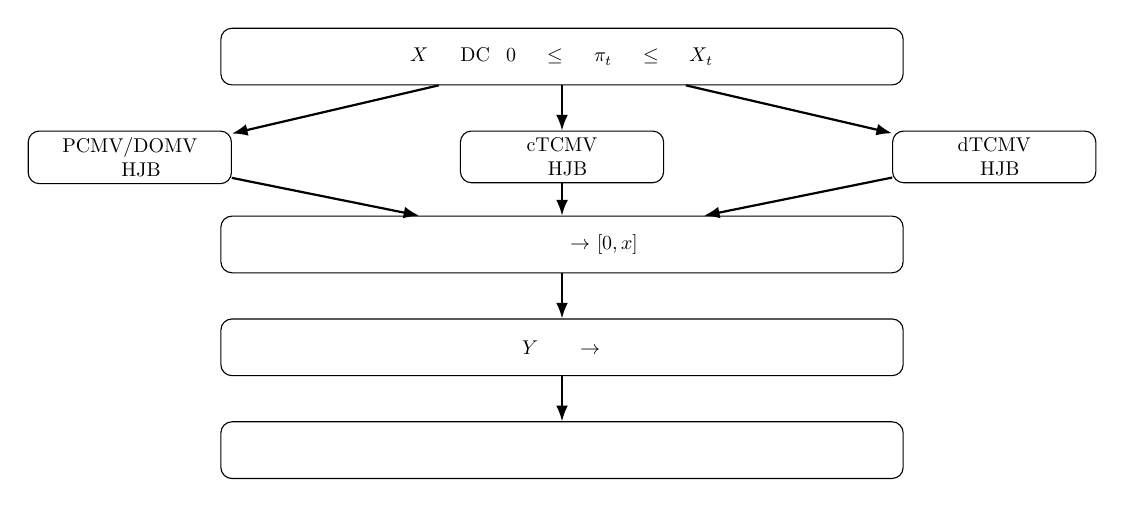
\begin{tikzpicture}[scale=0.72,transform shape,
  box/.style={rectangle,rounded corners,draw=black,align=center,text width=11.8cm,minimum height=1.0cm},
  small/.style={rectangle,rounded corners,draw=black,align=center,text width=3.35cm,minimum height=.85cm},
  arr/.style={-{Latex[length=2mm]},thick}
]
\node[box] (model) {$X$空間の実際のDC問題：$0\leq\pi_t\leq X_t$};
\node[small,below left=0.8cm and -0.2cm of model] (pcmv) {PCMV/DOMV\\二次損失HJB};
\node[small,below=0.8cm of model] (ctc) {cTCMV\\拡張HJB};
\node[small,below right=0.8cm and -0.2cm of model] (dtc) {dTCMV\\拡張HJB};
\node[box,below=2.3cm of model] (proj) {厳密制約フィードバック：制約付き継続価値 $\rightarrow$ $[0,x]$への局所射影};
\node[box,below=0.8cm of proj] (compare) {別の実装近似：$Y$空間の無制約解 $\rightarrow$ 事後クリップ};
\node[box,below=0.8cm of compare] (num) {射影差，自由境界，終端・ローリング分布により両方策を比較};
\draw[arr] (model) -- (pcmv);
\draw[arr] (model) -- (ctc);
\draw[arr] (model) -- (dtc);
\draw[arr] (pcmv) -- (proj);
\draw[arr] (ctc) -- (proj);
\draw[arr] (dtc) -- (proj);
\draw[arr] (proj) -- (compare);
\draw[arr] (compare) -- (num);
\end{tikzpicture}
\end{center}

\section{制約付きMV制御の統一Markov--Gauss--Hermiteエンジン}\label{sec:numerical-method}
\label{sec:numerical-bridge}
\label{sec:position}

\subsection{計算エンジンの位置づけと貢献}
\label{sec:gh-positioning}
前章で定式化した四つの制約付きMV問題を，同一条件で後退計算・前進評価するため，本稿はGauss--Hermite条件付き期待値，格子上の動的計画および確率質量伝播を共通化する．ここでいう\emph{統一Markov--Gauss--Hermiteエンジン}は新しい求積公式ではなく，標準的な数値部品を四解概念，厳密制約解とクリップ近似，終端分布，ローリング条件付き分布およびMV/MVS入れ子検証へ一貫して用いる計算アーキテクチャである．



本稿では，Gauss--Hermite条件付き期待値，格子上の後退計算，および確率質量の前進伝播を組み合わせた計算アーキテクチャを，便宜上\emph{統一Markov--Gauss--Hermiteエンジン}と呼ぶ．この名称は，新しい求積公式，Markov連鎖近似，半Lagrange法または一般的な動的計画法を発明したことを意味しない．Gauss--Hermite求積は標準的な決定論的数値積分であり\citep{AbramowitzStegun1972,Judd1998}，制御拡散に対するMarkov近似および半Lagrange型後退計算にも確立した一般論がある\citep{KushnerDupuis2001,FalconeFerretti2014}．MV資産配分に対するHJB数値解も先行研究に存在する\citep{WangForsyth2012,WangForsyth2012Comparison}．

したがって，本稿の数値的独自性は，個々の構成要素そのものにあるのではない．\emph{同じ一時点先期待値評価器と，そこから誘導される同じ離散遷移核とを，何に対して共通に用いるか}という点にある．表\ref{tab:gh-engine-positioning}は，既存部分と本稿固有の統合を分離する．

\begin{table}[H]
\centering\small
\caption{統一Markov--Gauss--Hermiteエンジンの位置づけ}
\label{tab:gh-engine-positioning}
\begin{tabularx}{\textwidth}{p{34mm}p{43mm}X}
\toprule
構成要素 & 方法論上の位置づけ & 本稿における機能と貢献 \\
\midrule
Gauss--Hermite条件付き期待値
& 正規ショックに対する標準的な決定論的求積
& PCMV，DOMV，cTCMV，dTCMVおよびMVS拡張で，同じ一時点先期待値評価器を用いる．目的関数が異なっても，ショック近似と補間規則を共通化する．\\
Markov・半Lagrange型後退計算
& 確率制御問題を格子上で解く既存の一般的方法
& 状態依存区間 $[0,x]$ を各格子点の許容集合へ直接入れ，通常のベルマン再帰と拡張HJBのモーメント再帰を一つの計算構造で扱う．\\
厳密制約フィードバックとクリップ近似の並列評価
& クリップ自体は実装容易な事後射影であり，厳密制約フィードバックとは別問題
& 厳密制約フィードバックとクリップ近似を同じ状態・制御格子，同じ求積節点，同じ補間および同じ前進評価器で比較し，射影差を方策構成の差として識別する．\\
同一核による前進分布伝播
& Markov遷移による確率質量伝播は標準的
& 後退計算で用いた遷移核をそのまま終端分布とローリング条件付き分布へ用い，密度，CDF，分位点，下方裾およびモーメント整合性を一貫して評価する．\\
四解概念・MV/MVSの共通実装
& 個別手法ではなく本稿の統合的設計
& 時間的意思決定原理の異なる四解概念とMVS入れ子拡張を，同じ入力・出力・診断形式へ載せ，数理的特徴づけを三層の実装判断へ接続する．\\
\bottomrule
\end{tabularx}
\end{table}

この共通化は，次の四つの役割を持つ．第一に，\emph{比較の識別}である．解概念間または厳密制約フィードバックとクリップ近似の結果差を比較するとき，条件付き期待値の計算法，乱数シードおよび前進分布の評価法を固定するため，差を主として目的関数・時間整合性・方策構成へ帰属できる．第二に，\emph{理論から加入者成果への橋渡し}である．検証定理が特徴づける局所フィードバックを，終端富分布，下方裾およびローリング条件付き分布まで同じ核で伝播できる．第三に，\emph{自由境界と射影差の再現可能な診断}である．内側ループに乱数モンテカルロ法を置かないため，候補制御間の小さな差や制約境界の位置が標本ノイズで変動しない．第四に，\emph{数値ガバナンス}である．後退モーメントと前進分布の整合性，確率質量保存，$\eta=0$におけるMVへの入れ子回帰検証などを，同じソフトウェア構造の中で実行できる．

\noindent\textbf{数値的貢献の主張範囲．}
本稿が主張するのは，新しい「Gauss--Hermite法」そのものではない．主張するのは，標準的な数値部品を統合した一つの後退・前進アーキテクチャである．この統合には，四つの制約付きMV解概念，厳密制約フィードバックとクリップ近似の比較，MV/MVS入れ子，後退方策計算，終端・ローリング分布の前進評価，および実務ガバナンスという六つの用途が含まれる．また，本稿の前進計算は，個別パスを乱数生成するモンテカルロ・シミュレーションではない．求積節点から作る離散遷移核に沿って，確率質量を決定論的に伝播する分布伝播法である．

\paragraph{Gauss--Hermite法を用いる理由．}
本稿では，各時点・状態・候補制御について条件付き期待値を反復評価するため，内側ループに標本ノイズを持ち込まないGauss--Hermite求積を用いる．同じ求積節点から得る離散遷移核を前進伝播にも用いることで，方策，自由境界，終端分布およびローリング分布を再現可能に評価する．

\subsection{数値状態空間と制御}
\label{sec:grid}

\paragraph{離散添字の記法．}
本節では，連続時間での状態の並び $(t,x)$ を離散化後も保つ．すなわち，例えば $V_n(x_i):=V(t_n,x_i)$，$M_n(x_i):=M(t_n,x_i)$，$\pi_n(x_i):=\pi(t_n,x_i)$ と書き，時点添字 $n$ は関数側に，$x_i$ は現在の残高格子点として表す．確率質量は $p_{n,i}$，制御格子の添字は $a$，Gauss--Hermite節点の添字は $k$，ローリング評価における戦略の添字は $j$ とする．状態 $(t_n,x_i)$ から候補制御 $\pi$ と第 $k$ Gauss--Hermite節点によって生成される次時点候補点は $\widehat{x}_{n+1}^{(k)}(x_i,\pi)$ と表す．

\subsubsection{時間格子}

時間区間 $[0,T]$ を $N_t$ 分割し，
\begin{equation}
  t_n=n\Delta t,
  \qquad
  \Delta t=\frac{T}{N_t},
  \qquad n=0,1,\ldots,N_t
  \label{eq:time-grid}
\end{equation}
とする．本文の基準計算は，40年間の拠出と運用見直しを月次で行う離散時間モデルとして $N_t=480$（$\Delta t=1/12$）を採用する．これは制度上の意思決定頻度に対応するモデル仕様であり，連続HJBの厳密な数値収束を保証しているわけではない．多数のパラメータを横断する感応度分析では計算負荷を抑えるため $N_t=80$ の粗選別仕様を用いるが，その結果を $N_t=480$ の精度保証には用いない．後退計算は $n=N_t-1,N_t-2,\ldots,0$ の順に，分布伝播は $n=0,1,\ldots,N_t-1$ の順に実行する．

\subsubsection{富格子}

DC口座残高 $X_t$ の格子を
\begin{equation}
  0=x_0<x_1<\cdots<x_I=x_{\max}
  \label{eq:wealth-grid}
\end{equation}
とし，残高格子点数を $N_x=I+1$ とする．等間隔格子の場合は $x_i=i\Delta x$ である．ただし，DC口座残高は低残高領域で制約が強く効くため，本稿では低残高側を細かくする非一様格子を用いる．具体的には
\begin{equation}
  x_i=x_{\max}\left(\frac{i}{I}\right)^\kappa,
  \qquad \kappa>1
  \label{eq:nonuniform-grid}
\end{equation}
とし，さらに決定論的初期残高 $x_0^{\mathrm{init}}=1/12$ を格子点として明示的に含める．$\kappa>1$ とすると $x=0$ 近傍に格子点が集中する．多数のシナリオを比較する感応度分析では $(I+1,\kappa)=(101,2.5)$ とし，最初の正の格子点は約 $0.003$，初期残高そのものも格子上に置く．本文の月次基準計算は，これよりさらに細かい151点格子を用いる．

低残高領域の細分化は単なる計算上の好みではない．第一に，許容投資額区間 $[0,x]$ は $x\downarrow0$ とともに縮退し，投資額 $\pi$ の小さな補間誤差が比率 $g=\pi/x$ では大きく増幅される．第二に，$x=0$ では全ての比率候補が同じ投資額 $\pi=0$ を与えるため，比率は経済的に識別されず，実装上の同点処理によって便宜的に0が選ばれ得る．第三に，dTCMVでは $\Gamma(t,x)=\rho_d/(x+H_t)$ が状態に依存するため，低残高点の制御誤差が背景富と上限制約の相互作用を通じて後続時点へ伝播する．したがって，最初の正の格子点が初期残高より大幅に高い粗い格子では，$x=0$ と遠い正の格子点の間の補間により，加入初期のリスク資産比率を人工的に0へ押し下げることがある．本稿では，低残高側の密格子，初期残高の明示的包含，および比率ではなく投資額 $\pi=xg$ の補間を組み合わせてこの人工物を除く．

本稿のPDEおよび分布伝播は，すべて $X$空間格子上で計算する．dTCMVについてのみ，背景富をリスク許容度に反映するため，評価関数内で
\begin{equation}
  \Gamma(t_n,x_i)=\frac{\rho_d}{x_i+H_{t_n}}
  \label{eq:gamma-grid}
\end{equation}
を用いる．$H_{t_n}$ は外生的に後退計算される確定量であり，新たな状態次元や $Y$空間格子を導入しない．また，$\alpha$ による部分背景富の一般化は行わない．

\subsubsection{制御格子と許容区間}

各格子点 $(t_n,x_i)$ における許容制御は
\begin{equation}
  \Pi_{n,i}=[0,x_i]
  \label{eq:control-interval}
\end{equation}
である．数値的には，候補制御を
\begin{equation}
  \pi_i^{(a)}=\frac{a}{N_a-1}x_i,
  \qquad a=0,1,\ldots,N_a-1
  \label{eq:control-grid}
\end{equation}
として離散化する．より高精度にする場合は，局所ハミルトニアンまたは離散目的関数が二次に近いことを用いて，粗い候補探索の後に1次元の黄金分割探索またはBrent法で $[0,x_i]$ 上の最大化・最小化を行う．

\begin{remark}[制御格子と射影公式]
前節の理論では，滑らかな値関数またはモーメント関数が与えられたとき，厳密制約フィードバックが局所無制約候補を $[0,x]$ に射影する形で表されることを示した．しかし数値実装では，射影公式だけに依存する必要はない．候補制御を $[0,x_i]$ 上で直接探索すれば，境界拘束領域でも非拘束領域でも同じ手順で計算できる．射影公式は，計算結果を診断し，自由境界と射影差を解釈するために使う．
\end{remark}

\subsection{Gauss--Hermite条件付き期待値}
\label{sec:gh}

ここまでで，無制約問題の陽な制御式と，厳密制約問題における状態依存フィードバックおよび制約拘束領域の構造はほぼ出そろっている．一方，実際の数値計算では，HJB方程式または拡張HJB方程式系の継続価値を評価する必要が残る．予備的に有限差分法でこれらの偏微分方程式を直接解いたところ，時間・状態メッシュや微分近似への感応度が無視できず，とくに切替境界付近では，滑らかに見える数値解であっても，その局所的な形状が真の制御問題に由来するのか，メッシュ上の人工的な揺らぎなのかを判別しにくかった．この経験から，本稿の主たる数値計算では，HJB偏微分方程式を有限差分で直接解く方法とは別のアプローチを採用する．

具体的には，1期間先の条件付き期待値を直接評価し，そこから得られる遷移核を用いて動学的な後退計算を構成する．正規ショックはGauss--Hermite求積で評価し，同一の遷移核を後退計算と前進確率質量伝播の双方に用いる．さらに，格子精緻化，境界質量診断，および後退モーメントと前進分布の整合性によって数値解を検証する．もちろん離散化誤差そのものが消えるわけではないが，PDEの空間微分を直接差分化する際の不透明な感応度を，時間・状態・制御格子，補間，求積次数という個別に監視可能な誤差へ置き換えることができる．

\subsubsection{1期間遷移}

時点 $t_n$，状態 $x_i$，候補制御 $\pi$ の下で，Euler近似により次時点のDC口座残高を
\begin{equation}
  X_{n+1}^{\pi}
  =x_i+(rx_i+c_n+\beta\pi)\Delta t+\sigma\pi\sqrt{\Delta t}\,Z,
  \qquad Z\sim N(0,1)
  \label{eq:euler-transition}
\end{equation}
とする．ここで $c_n=c_{t_n}$ である．$Z$ の期待値を乱数で評価する代わりに，$K$ 点Gauss--Hermite求積を用いる．

標準的なHermite多項式の節点・重みを $(z_k,\omega_k)_{k=1}^K$ とし，
\begin{equation}
  \int_{-\infty}^{\infty} e^{-z^2}f(z)\dd z
  \approx
  \sum_{k=1}^K\omega_k f(z_k)
  \label{eq:gh-basic}
\end{equation}
を用いる．標準正規 $Z$ に対する期待値は
\begin{equation}
  \E[f(Z)]
  =\frac{1}{\sqrt{\pi}}\int_{-\infty}^{\infty}e^{-z^2}f(\sqrt{2}z)\dd z
  \approx
  \sum_{k=1}^K w_k f(\xi_k),
  \label{eq:gh-normal}
\end{equation}
で近似する．ここで
\begin{equation}
  \xi_k=\sqrt{2}z_k,
  \qquad
  w_k=\frac{\omega_k}{\sqrt{\pi}},
  \qquad
  \sum_{k=1}^K w_k=1
  \label{eq:gh-nodes}
\end{equation}
である．

したがって，一時点先の候補点は
\begin{equation}
  \widehat{x}_{n+1}^{(k)}(x_i,\pi)
  =x_i+(rx_i+c_n+\beta\pi)\Delta t
  +\sigma\pi\sqrt{\Delta t}\,\xi_k,
  \qquad k=1,\ldots,K
  \label{eq:transition-gh-nodes}
\end{equation}
となる．

\subsubsection{補間作用素}

$V_{n+1}(x)$ の格子値が既知であるとき，$\widehat{x}_{n+1}^{(k)}(x_i,\pi)$ は一般に格子点と一致しない．そこで線形補間作用素 $\mathcal I_{n+1}$ を用い，
\begin{equation}
  \E\left[V_{n+1}(X_{n+1}^{\pi})\mid X_n=x_i\right]
  \approx
  \sum_{k=1}^K w_k\,
  \bigl(\mathcal I_{n+1}V_{n+1}\bigr)
  \left(\widehat{x}_{n+1}^{(k)}(x_i,\pi)\right)
  \label{eq:gh-expectation}
\end{equation}
と評価する．非一様格子の場合も，同じく隣接する格子点間の線形補間を用いる．必要に応じて単調性を保つ形状保存補間を用いるが，高次補間はHJBの単調性を損なう可能性があるため，基準実装では線形補間を採用する．

\subsection{PCMVとDOMVの埋め込み二次損失HJB}
\label{sec:embedded}

\subsubsection{連続時間偏微分方程式}

PCMVおよびDOMVの数値計算は，平均制約または目標パラメータを持つ埋め込み二次損失問題を出発点にする．代表的には，終端ターゲット $m$ に対して
\begin{equation}
  V(t,x;m)=\inf_{\pi\in\A^X_{t,x}}
  \E_{t,x}\left[(X_T+D_T-m)^2\right]
  \label{eq:embedded-value}
\end{equation}
を解く．$D_T$ は，退職時点の確定的終端給付を表す．$D_T$ が確定であれば，終端条件は
\begin{equation}
  V(T,x;m)=(x+D_T-m)^2
  \label{eq:embedded-terminal}
\end{equation}
である．形式的なHJBは
\begin{equation}
  V_t+
  \inf_{0\leq\pi\leq x}
  \left\{
    (rx+c_t+\beta\pi)V_x
    +\frac{1}{2}\sigma^2\pi^2 V_{xx}
  \right\}=0,
  \qquad
  V(T,x)=(x+D_T-m)^2.
  \label{eq:embedded-hjb}
\end{equation}

局所ハミルトニアンを
\begin{equation}
  \Hamil^Q(t,x,\pi;V)
  =(rx+c_t+\beta\pi)V_x
  +\frac{1}{2}\sigma^2\pi^2 V_{xx}
  \label{eq:quadratic-ham}
\end{equation}
と置く．$V_{xx}>0$ の領域では，無制約候補は
\begin{equation}
  \pi^{\mathrm{loc}}(t,x)
  =-\frac{\beta V_x(t,x)}{\sigma^2 V_{xx}(t,x)}
  \label{eq:loc-pi-quadratic}
\end{equation}
であり，厳密制約フィードバックは
\begin{equation}
  \pi^{\mathrm{str}}(t,x)
  =\Proj_{[0,x]}\left(\pi^{\mathrm{loc}}(t,x)\right)
  \label{eq:proj-quadratic}
\end{equation}
として診断できる．ただし，実際の数値計算では，\eqref{eq:embedded-hjb} を有限差分またはMarkov--GH後退計算で直接解く．

\subsubsection{Markov--Gauss--Hermite後退計算}

Gauss--Hermite版の後退計算は，偏微分方程式\eqref{eq:embedded-hjb}の半Lagrange近似として書ける．終端条件を
\begin{equation}
  V_{N_t}(x_i;m)=(x_i+D_T-m)^2
  \label{eq:terminal-discrete-quad}
\end{equation}
とし，$n=N_t-1,\ldots,0$ について
\begin{equation}
  V_n(x_i;m)=
  \min_{\pi\in[0,x_i]}
  \sum_{k=1}^K w_k\,
  \bigl(\mathcal I_{n+1}V_{n+1}(\cdot;m)\bigr)
  \left(\widehat{x}_{n+1}^{(k)}(x_i,\pi)\right),
  \qquad n=N_t-1,\ldots,0
  \label{eq:quad-backward-gh}
\end{equation}
を計算する．同時に，最小化を達成する制御を
\begin{equation}
  \pi_n^{\mathrm{QL}}(x_i;m)=
  \argmin_{\pi\in[0,x_i]}
  \sum_{k=1}^K w_k\,
  \bigl(\mathcal I_{n+1}V_{n+1}(\cdot;m)\bigr)
  \left(\widehat{x}_{n+1}^{(k)}(x_i,\pi)\right)
  \label{eq:quad-feedback-gh}
\end{equation}
として保存する．この $\pi_n^{\mathrm{QL}}(x_i;m)$ が，埋め込み二次損失問題に対する厳密制約フィードバックである．上付き $\mathrm{QL}$ は二次損失（quadratic loss）の方策を表し，二次モーメント関数 $Q$ と区別する．

\begin{remark}[半Lagrange解釈]
式\eqref{eq:quad-backward-gh} は，拡散項を有限差分で直接近似するのではなく，一時点先の遷移分布に沿って値関数を補間し，条件付き期待値を求める半Lagrange型の近似である．HJBを微分演算子として離散化する陰的有限差分法と異なり，候補制御ごとの遷移が直感的で，制約 $0\leq\pi\leq x$ も自然に入る．本稿では，このMarkov--GH型を唯一の基準実装とし，同一の離散遷移核を後退計算と前進分布伝播に用いる．
\end{remark}

\subsubsection{スカラー化MV目的の下でのPCMV目標整合}

PCMVを目標平均 $m_0^{\mathrm{tar}}$ により定義する場合は，保存済みフィードバック $\pi^{\mathrm{QL}}(m)$ の下で
\[
  \mu^m(t,x):=\E_{t,x}^{\pi^{\mathrm{QL}}(m)}[X_T+D_T]
\]
を計算し，$\mu^m(0,x_0)=m_0^{\mathrm{tar}}$ を満たす $m$ を探索すればよい．一方，DOMVと同一の分散回避係数で比較する数値実験では，スカラー化目的
\[
  \E[W_T]-\frac{\gamma}{2}\Var(W_T),
  \qquad W_T=X_T+D_T,
\]
を二次損失へ埋め込む．固定ターゲット $m$ の値関数を式\eqref{eq:embedded-value}とすると，
\begin{equation}
  \sup_{\pi}
  \left\{\E[W_T]-\frac{\gamma}{2}\Var(W_T)\right\}
  =\sup_{m\in\mathbb R}
  \left\{
    m-\frac{1}{2\gamma}-\frac{\gamma}{2}V(t,x;m)
  \right\}.
  \label{eq:scalarized-embedded-pcmv}
\end{equation}
内点解では
\begin{equation}
  m^*(t,x)=\mu^{m^*}(t,x)+\frac{1}{\gamma}
  \label{eq:embedded-fixed-point}
\end{equation}
が成立する．PCMVでは式\eqref{eq:scalarized-embedded-pcmv}を $(0,x_0)$ で一度だけ最大化し，得られた $m_P^*$ の固定ターゲット・フィードバックへ満期までコミットする．

\subsubsection{ローリング目標選択としてのDOMV}

DOMVでは，各時点・各状態において，残存期間 $[t,T]$ のMV問題
\begin{equation}
  \sup_{\pi\in\A^X_{t,x}}
  \left\{
    \E_{t,x}[W_T]
    -\frac{\gamma_D}{2}\Var_{t,x}(W_T)
  \right\}
  \label{eq:domv-discrete-problem}
\end{equation}
を解き直す．数値実装では，候補ターゲット集合 $\mathcal M=\{m_1,\ldots,m_{N_m}\}$ の各 $m_\ell$ について，$m_\ell$ を残存期間全体で固定した二次損失問題\eqref{eq:quad-backward-gh}を解く．その後，各格子点で
\begin{equation}
  m_D^*(t_n,x_i)
  \in\argmax_{m_\ell\in\mathcal M}
  \left\{
    m_\ell-\frac{1}{2\gamma_D}
    -\frac{\gamma_D}{2}V_n(x_i;m_\ell)
  \right\}
  \label{eq:domv-target-grid-selection}
\end{equation}
を選び，対応する固定ターゲット問題の最初の制御
\begin{equation}
  \pi_n^{\mathrm{DOMV}}(x_i)
  =\pi_n^{\mathrm{QL}}\!\left(x_i;m_D^*(t_n,x_i)\right)
  \label{eq:domv-first-control}
\end{equation}
だけを採用する．次時点では，新しい状態から式\eqref{eq:domv-target-grid-selection}を再評価する．

重要なのは，候補 $m_\ell$ を評価する後退計算の途中では，そのターゲットを別の $m_k$ に変更しないことである．途中で状態依存ターゲットへ切り替えると，$\E[(W_T-m_\ell)^2]$ という固定ターゲット問題を評価したことにならず，ローリングDOMVとも異なるヒューリスティックになる．本稿の\emph{ターゲット格子近似}は，複数の固定ターゲット問題を完結に解いた後で，現在の時点・状態における最初の制御を選択する方法を指す．

ターゲット格子近似については，式\eqref{eq:embedded-fixed-point}に対応する平均整合誤差と，探索範囲端点が選択されていないことを確認する．ターゲット刻みを独立に細分化した包括的な格子安定性分析は今後の課題とする．

\subsection{cTCMVとdTCMVの拡張HJBソルバー}
\label{sec:extended}

\subsubsection{モーメント関数}

時間整合的MVでは，目的関数が
\begin{equation}
  J(t,x)=M(t,x)-\frac{\Gamma(t,x)}{2}
  \left(Q(t,x)-M(t,x)^2\right)
  \label{eq:tc-objective}
\end{equation}
の形を持つ．ここで
\begin{align}
  M(t,x)&=\E_{t,x}^{\pi^*}[X_T+D_T],\label{eq:M-def}\\
  Q(t,x)&=\E_{t,x}^{\pi^*}[(X_T+D_T)^2]\label{eq:Q-def}
\end{align}
であり，$\pi^*$ は均衡フィードバック制御則である．cTCMVでは
\begin{equation}
  \Gamma(t,x)=\gamma_c
  \label{eq:gamma-c}
\end{equation}
を定数とし，dTCMVでは
\begin{equation}
  \Gamma(t,x)=\frac{\rho_d}{x+H_t}
  \label{eq:gamma-d}
\end{equation}
とする．ここで $H_t$ は将来拠出および確定的背景年金富の現在価値である．

\subsubsection{離散1期間均衡条件}

時点 $t_n$，状態 $x_i$ において，時点 $t_n$ から $t_{n+1}$ までだけ候補制御 $\pi$ を用い，その後は既に後退計算で求めた均衡フィードバック制御則に従うとする．このとき候補制御 $\pi$ の下での一時点先評価は
\begin{align}
  M_n(x_i;\pi)
  &=\sum_{k=1}^K w_k\,
  \bigl(\mathcal I_{n+1}M_{n+1}\bigr)
  \left(\widehat{x}_{n+1}^{(k)}(x_i,\pi)\right),
  \label{eq:Mpi-gh}\\
  Q_n(x_i;\pi)
  &=\sum_{k=1}^K w_k\,
  \bigl(\mathcal I_{n+1}Q_{n+1}\bigr)
  \left(\widehat{x}_{n+1}^{(k)}(x_i,\pi)\right)
  \label{eq:Qpi-gh}
\end{align}
したがって，一時点逸脱に対する離散時間の均衡目的関数は
すなわち，
\begin{equation}
  \Psi_n(x_i;\pi)
  =M_n(x_i;\pi)
  -\frac{\Gamma(t_n,x_i)}{2}
  \left(Q_n(x_i;\pi)-M_n(x_i;\pi)^2\right)
  \label{eq:Psi-pi-clean}
\end{equation}
である．均衡フィードバック制御則は
\begin{equation}
  \pi_n^{\mathrm{TC}}(x_i)
  \in\argmax_{\pi\in[0,x_i]}\Psi_n(x_i;\pi)
  \label{eq:tc-feedback-discrete}
\end{equation}
で定義される．フィードバックを決めた後，
\begin{align}
  M_n(x_i)&=M_n\!\left(x_i;\pi_n^{\mathrm{TC}}(x_i)\right),
  \label{eq:M-update-TC}\\
  Q_n(x_i)&=Q_n\!\left(x_i;\pi_n^{\mathrm{TC}}(x_i)\right),
  \label{eq:Q-update-TC}\\
  J_n(x_i)&=M_n(x_i)-\frac{\Gamma(t_n,x_i)}{2}
  \left(Q_n(x_i)-M_n(x_i)^2\right)
  \label{eq:J-update-TC}
\end{align}
と更新する．終端条件は
\begin{equation}
  M_{N_t}(x_i)=x_i+D_T,
  \qquad Q_{N_t}(x_i)=(x_i+D_T)^2,
  \qquad J_{N_t}(x_i)=x_i+D_T
  \label{eq:tc-terminal}
\end{equation}
である．

\begin{remark}[拡張HJBとの関係]
式\eqref{eq:tc-feedback-discrete} は，連続時間の均衡定義における短時間逸脱に対応する，離散時間版の一時点逸脱条件である．$\Delta t\to0$，$\Delta x\to0$，Gauss--Hermite次数 $K\to\infty$ の極限では，前節で記述した拡張HJB系の局所最大化条件に対応する．本稿では，解析的な微分係数から直接ハミルトニアンを組み立てるのではなく，$M,Q$ の一時点先条件付き期待値をGauss--Hermiteで直接評価するため，低残高領域や境界近傍でも比較的安定に計算できる．
\end{remark}

\subsubsection{cTCMVとdTCMVの均衡アルゴリズム}
両均衡概念とも，終端モーメントを $M_{N_t}(x_i)=x_i+D_T$ および $Q_{N_t}(x_i)=(x_i+D_T)^2$ と置き，後退計算する．各節点・各許容制御について，Gauss--Hermite求積により1期間条件付きモーメントを評価し，1期間逸脱目的を最大化して，最大化制御と誘導モーメントを保存する．構造上の違いは分散回避係数だけである：
\begin{equation}
\Gamma_{n,i}=\gamma_c\quad\text{（cTCMVの場合）},
\qquad
\Gamma_{n,i}=\frac{\rho_d}{x_i+H_{t_n}}\quad\text{（dTCMVの場合）}.
\label{eq:gamma-grid-compact}
\end{equation}
したがって，同じソルバーが標準デフォルト層と総年金富に基づく個別化助言層を処理し，dTCMVでは状態・時間依存の総年金富スケーリングのみが追加される．完全な擬似コードは本文で反復せず，再現パッケージに収録する．




\subsubsection{共通数値エンジンにおけるCPベンチマーク}

CPについては後退HJBを解かず，各格子時点で式\eqref{eq:cp-policy}をそのまま用い，最適戦略と同じGauss--Hermite遷移核で確率質量を前進伝播する．したがって，CPと四つのMV戦略の差は乱数シードや分布計算法の差ではなく，フィードバック則の差に由来する．共通平均比較では，期待終端富が四つのMV戦略と一致するように $\theta_{cp}$ を数値的に較正する．

\begin{remark}[基準計算では方策反復を用いない]
本稿の基準計算は，Markov--Gauss--Hermite後退計算と許容区間 $[0,x]$ 上の直接探索である．PCMV/DOMVの各固定ターゲット問題は通常の動的計画再帰として解き，cTCMV/dTCMVは式\eqref{eq:tc-feedback-discrete}の一時点逸脱条件を直接最大化する．したがって，陰的有限差分方程式に対するHoward型方策反復法は基準結果には用いない．独立ソルバー比較を提示しない限り，方策反復法の一般論を本文へ追加することは，実際の計算方法を不明確にするため避ける．
\end{remark}

\subsection{厳密制約フィードバックとクリップ近似の数値実装}
\label{sec:projection-gap}

節\ref{sec:strict-clip}で区別した二つの実装可能方策を，同じ格子と同じ前進分布エンジンで評価する．厳密制約フィードバックは，上で定義した各解概念固有の後退問題から得る．すなわち，PCMVは時点0で選択した固定ターゲットの二次損失最小化，DOMVは各状態で再選択したターゲット，cTCMV・dTCMVは1期間均衡目的の最大化に基づく．共通記号では
\begin{equation}
  \pi_n^{\mathrm{str}}(x_i)
  =
  \begin{cases}
    \pi_n^{\mathrm{QL}}(x_i;m_P^*), & \text{PCMV},\\
    \pi_n^{\mathrm{DOMV}}(x_i), & \text{DOMV},\\
    \pi_n^{\mathrm{TC}}(x_i), & \text{cTCMV・dTCMV},
  \end{cases}
  \label{eq:pi-str-def}
\end{equation}
と書ける．cTCMVとdTCMVの違いは，各々の $\Gamma(t_n,x_i)$ によって表される．一方，クリップ近似は，節\ref{sec:strict-clip}の$Y$空間における無制約解を用いて
\begin{equation}
  \pi_n^{\mathrm{clip}}(x_i)
  =\Proj_{[0,x_i]}\!\left(\pi^{\mathrm{unc}}(t_n,x_i+H_{t_n})\right)
  \label{eq:pi-clip-def}
\end{equation}
と構成する．前者は制約付き継続価値を再帰的に計算するが，後者は無制約継続価値を変えずに現在制御のみを切り詰める．

両方策についてそれぞれ独立に確率質量を前進伝播する．したがって，射影差は同じ状態点での制御差だけでなく，方策差が将来の到達残高分布を変える効果も終端・ローリング分布へ反映する．

\subsubsection{射影差の指標}

厳密制約フィードバックとクリップ近似の差を，次の指標で測る．

\begin{align}
  \Delta\pi_n(x_i)
  &=\pi_n^{\mathrm{str}}(x_i)-\pi_n^{\mathrm{clip}}(x_i),
  \label{eq:delta-pi}\\
  \Delta g_n(x_i)
  &=\frac{\pi_n^{\mathrm{str}}(x_i)}{x_i}
  -\frac{\pi_n^{\mathrm{clip}}(x_i)}{x_i},
  \qquad x_i>0
  \label{eq:delta-g}
\end{align}

さらに，前進分布 $p_{n,i}$ で重み付けした平均絶対差を
\begin{equation}
  \mathrm{PG}_{\mathrm{WMAE}}
  =\frac{1}{N_t}
  \sum_{n=0}^{N_t-1}\sum_{i=1}^{I}
  p_{n,i}^{\mathrm{str}}\,|\Delta g_n(x_i)|
  \label{eq:pg-wmae}
\end{equation}
と定義する．ここで $p_{n,i}^{\mathrm{str}}$ は厳密制約フィードバック自身が誘導する前進分布であり，$\mathrm{PG}_{\mathrm{WMAE}}$ は基準となるstrict方策の下で実際に到達しやすい領域における平均的な射影差を表す．表\ref{tab:tcmv-projection-gap}の「加重平均絶対差」は式\eqref{eq:pg-wmae}に対応する．

\subsubsection{自由境界の分類}

各ノードを次の三領域に分類する．

\begin{align}
  \mathcal R_0&=\{(n,i):\pi_n^{\mathrm{str}}(x_i)=0\},\label{eq:R0}\\
  \mathcal R_I&=\{(n,i):0<\pi_n^{\mathrm{str}}(x_i)<x_i\},\label{eq:RI}\\
  \mathcal R_U&=\{(n,i):\pi_n^{\mathrm{str}}(x_i)=x_i\}.\label{eq:RU}
\end{align}
$\mathcal R_0$ はリスク資産を持たない領域，$\mathcal R_I$ は内点領域，$\mathcal R_U$ はDC残高全額をリスク資産に投資する上限制約拘束領域である．自由境界は，$\mathcal R_I$ と $\mathcal R_0$ または $\mathcal R_U$ の境目として数値的に定義する．数値分析では，厳密制約フィードバックの自由境界とクリップ近似の拘束状態を区別して可視化する．

\subsection{乱数モンテカルロを用いない前進分布伝播}
\label{sec:forward}

\subsubsection{富格子上の確率質量伝播}

フィードバック $\pi_n^*(x_i)$ が後退計算で得られた後，終端富分布を評価する．通常は乱数モンテカルロにより多数のパスを発生させるが，本稿ではGauss--Hermite遷移を用いて確率質量を前進伝播する．

初期分布を
\begin{equation}
  p_{0,i}=\one_{\{x_i=x_0\}}
  \label{eq:initial-mass}
\end{equation}
とする．$x_0$ が格子点に一致しない場合は，隣接格子点に線形補間で質量を配分する．時点 $n$ の質量 $p_{n,i}$ が与えられたとき，各状態 $x_i$ から各Gauss--Hermite節点 $k$ に対して
\begin{equation}
  \widehat{x}_{n+1}^{(k)}(x_i,\pi_n^*(x_i))
  =x_i+\bigl(rx_i+c_n+\beta\pi_n^*(x_i)\bigr)\Delta t
  +\sigma\pi_n^*(x_i)\sqrt{\Delta t}\,\xi_k
  \label{eq:forward-node}
\end{equation}
を計算する．この点を次時点格子に線形配分し，重み $p_{n,i}w_k$ を加える．すなわち，$x_{\ell}\leq \widehat{x}_{n+1}^{(k)}(x_i,\pi_n^*(x_i))\leq x_{\ell+1}$ なら
\begin{align}
  p_{n+1,\ell}&\leftarrow p_{n+1,\ell}
  +p_{n,i}w_k\frac{x_{\ell+1}-\widehat{x}_{n+1}^{(k)}(x_i,\pi_n^*(x_i))}{x_{\ell+1}-x_{\ell}},\label{eq:mass-left}\\
  p_{n+1,\ell+1}&\leftarrow p_{n+1,\ell+1}
  +p_{n,i}w_k\frac{\widehat{x}_{n+1}^{(k)}(x_i,\pi_n^*(x_i))-x_{\ell}}{x_{\ell+1}-x_{\ell}}
  \label{eq:mass-right}
\end{align}
$\widehat{x}_{n+1}^{(k)}(x_i,\pi_n^*(x_i))<0$ の遷移は下側境界 $x_0=0$ に，$\widehat{x}_{n+1}^{(k)}(x_i,\pi_n^*(x_i))>x_{\max}$ の遷移は上側境界に配分する．ただし，境界配分前に格子外へ出た確率質量は節\ref{sec:diagnostics}で別途記録する．これにより，乱数を使わずに $X_T$ の離散分布が得られる．終端総年金富は $X_T+D_T$ である．

\subsubsection{モーメントと裾リスク指標}

終端分布 $p_{N_t,i}$ から，以下の指標を計算する．
\begin{align}
  \widehat{\mu}_T&=\sum_i p_{N_t,i}(x_i+D_T),\label{eq:mean-terminal}\\
  \widehat{\sigma}_T^2&=\sum_i p_{N_t,i}\{(x_i+D_T)-\widehat{\mu}_T\}^2,\label{eq:var-terminal}\\
  \widehat{m}_{3,T}&=\sum_i p_{N_t,i}\{(x_i+D_T)-\widehat{\mu}_T\}^3.\label{eq:third-terminal}
\end{align}
分位点は，累積質量
\begin{equation}
  F_{N_t}(x_\ell)=\sum_{i\leq \ell}p_{N_t,i}
  \label{eq:cdf-terminal}
\end{equation}
から求める．$W_i=x_i+D_T$ と置き，$F_T^W(w):=\sum_{i:W_i\leq w}p_{N_t,i}$，$q_\tau:=\inf\{w:F_T^W(w)\geq\tau\}$ と定義する．前進伝播で得られる分布は離散分布であるため，分位点上の確率質量は裾確率がちょうど $\alpha$ となる分だけ含める．下方LCVaRは
\begin{equation}
  \mathrm{LCVaR}_\alpha
  =\frac{1}{\alpha}
  \left[
    \sum_{W_i<q_\alpha}p_{N_t,i}W_i
    +\left(\alpha-\sum_{W_i<q_\alpha}p_{N_t,i}\right)q_\alpha
  \right]
  \label{eq:lcvar}
\end{equation}
で近似する．上方参加を測るため，上位 $\alpha$ の条件付き平均を
\begin{equation}
  \mathrm{UCVaR}_\alpha
  =\frac{1}{\alpha}
  \left[
    \sum_{W_i>q_{1-\alpha}}p_{N_t,i}W_i
    +\left(\alpha-\sum_{W_i>q_{1-\alpha}}p_{N_t,i}\right)q_{1-\alpha}
  \right]
  \label{eq:ucvar}
\end{equation}
として併記する．

\subsubsection{経路依存グライドパスの要約}

Gauss--Hermite分布伝播では個別パスを発生させないため，パスごとの平均グライドパスは直接得られない．しかし，意思決定時点 $t_n$ における状態分布 $p_{n,i}$ とフィードバック $g_{n,i}=\pi^*_{n,i}/x_i$ から，$n\geq1$ では分布加重平均グライドパスを
\begin{equation}
  \bar g_n=\sum_{i:x_i>0}p_{n,i}\,g_n(x_i)
  \label{eq:mean-glidepath}
\end{equation}
として計算できる．一方，初期残高 $x_0=1/12$ は決定論的であり，状態格子の二点へ初期質量を分割して比率を平均すると，$x=0$ に便宜上置いた $g(0,0)=0$ が初期比率を人工的に押し下げる．そこで初期投資額を
\begin{equation}
  \pi_0=\Interp_{x}\!\left\{x_i g_0(x_i)\right\}(x_0),
  \qquad
  \bar g_0=\frac{\pi_0}{x_0}
  \label{eq:exact-initial-glide}
\end{equation}
とし，最初の一期間は正確な初期状態 $x_0$ から直接遷移させ，その遷移後の確率質量を状態格子へ配分する．すなわち，比率 $g$ ではなく投資額 $\pi=xg$ を補間することで，ゼロ残高点の便宜的定義が初期グライドパスへ混入することを防ぐ．

また，制御は区間 $[t_n,t_{n+1})$ に対して $n=0,\ldots,N_t-1$ でのみ定義され，終端時点 $T=t_{N_t}$ には新たな投資判断が存在しない．したがって，グライドパス図は意思決定時点 $t_0,\ldots,t_{N_t-1}=T-\Delta t$ のみを対象とし，未定義の終端制御をゼロで補完しない．終端制御を機械的にゼロで補完すると，退職直前のリスク削減と誤認され得る不連続が生じるためである．また， $p_{n,i}$ に基づいて $g_n(x_i)$ の中央値，10\%点，90\%点を求めることにより，加入者が経験し得るグライドパスの分布を示す．この方法はモンテカルロ法によるパス分位点に対応するが，乱数誤差を伴わない．

\subsection{ローリング条件付き評価}
\label{sec:rolling}

\subsubsection{ローリング条件付き成果指標の定義}

戦略 $j$ の保存済みフィードバックを，時点 $t$，現在残高 $x$ から満期まで継続したときの条件付き終端富を $W_T^{j;t,x}$ とする．本稿では，その残存期間成果を一つの平均--分散値へ集約せず，次の指標ベクトルで表す：
\begin{equation}
\begin{split}
 \mathbf O_j(t,x;\alpha)=\bigl(&\mu_j(t,x),\ s_j(t,x),\ q_{j,\alpha}(t,x),\ q_{j,0.50}(t,x),\ q_{j,1-\alpha}(t,x),\\
 &\operatorname{LCVaR}_{j,\alpha}(t,x),\ \operatorname{UCVaR}_{j,\alpha}(t,x),\ \operatorname{Skew}_j(t,x),\ g_j(t,x),\ \pi_j(t,x)\bigr),
 \label{eq:rolling-outcome-profile}
\end{split}
\end{equation}
ここで，$\mu_j$と$s_j$は $W_T^{j;t,x}$ の条件付き平均と標準偏差，$q_{j,\alpha}$は条件付き分位点，$g_j$と$\pi_j=xg_j$は現在のリスク資産比率と投資額である．以下では式\eqref{eq:rolling-outcome-profile}を\emph{ローリング条件付き成果指標}と呼ぶ．これは単一の順位を与えるスカラー指標ではなく，期待成果，上下方リスク，分布の非対称性および現在の行動を同時に示す多面的な成果プロファイルである．

\subsubsection{全期待値・全分散の公式による位置づけ}

戦略 $j$ の保存済みフィードバックの下で生じる時点 $t$ の残高を $X_t^j$，終端富を $W_T^j=X_T^j+D_T$ とする．また，状態固定型の条件付き平均と条件付き分散を
\begin{equation}
  \mu_j(t,x)=\E\!\left[W_T^j\mid X_t^j=x\right],
  \qquad
  v_j(t,x)=\Var\!\left(W_T^j\mid X_t^j=x\right)
  \label{eq:rolling-conditional-moments}
\end{equation}
と定義する．Markovフィードバックの下では，$\E[W_T^j\mid\mathcal F_t]=\mu_j(t,X_t^j)$ である．

\begin{proposition}[時点0評価とローリング条件付き評価の分解]
\label{prop:total-variance-rolling}
任意の $t\in[0,T]$ について，必要な二次モーメントが有限ならば，
\begin{align}
  \E[W_T^j]
  &=\E\!\left[\mu_j(t,X_t^j)\right],
  \label{eq:total-expectation-rolling}\\
  \Var(W_T^j)
  &=\E\!\left[v_j(t,X_t^j)\right]
    +\Var\!\left(\mu_j(t,X_t^j)\right)
  \label{eq:total-variance-rolling}
\end{align}
が成立する．
\end{proposition}

\begin{proof}
式\eqref{eq:total-expectation-rolling}は反復期待値の法則から従う．また，
\[
 W_T^j-\E[W_T^j]
 =\{W_T^j-\mu_j(t,X_t^j)\}
  +\{\mu_j(t,X_t^j)-\E[W_T^j]\}
\]
と分解し，$X_t^j$ を条件として交差項の条件付き期待値がゼロであることを用いれば，式\eqref{eq:total-variance-rolling}を得る．
\end{proof}

式\eqref{eq:total-variance-rolling}の第1項は，時点 $t$ の各残高状態から先に残る\emph{将来プロセスリスク}を，その時点の加入者分布で平均したものである．第2項は，時点 $t$ までの運用経験によって形成された残高差が，条件付き期待終端富の差として現れる\emph{状態間格差}である．時点0では $X_0=x_0$ が決定論的であるため第2項はゼロであり，時点0の終端分散は $v_j(0,x_0)$ に一致する．しかし途中時点では，一般に両項が正となり，時点0から見た総分散は「その後にも残るリスク」と「既に形成された加入者間格差」を同時に含む．

これに対し，現在残高を $x$ に固定するローリング条件付き評価は，$\mu_j(t,x)$，$v_j(t,x)$ および条件付き裾指標を直接評価する．したがって，この評価は，式\eqref{eq:total-variance-rolling}の第2項を過去に形成された状態差として固定したうえで，現在の評価日から先の意思決定に関係する条件付き分布を切り出す，と言い換えられる．なお，ローリング評価は無条件評価を否定するものではない．前者は制度開始時点の設計評価，後者は評価日時点で観測された加入者状態からの将来見通しであり，両者は全期待値・全分散の公式によって整合的に接続される．

共通平均の下でPCMVは，時点0における総終端分散を最小化するよう設計される．したがって，時点0の無条件比較でPCMVの分散圧縮が最も目立つことは目的関数上自然であり，PCMVの設計ベンチマークとしての価値を示す．一方，PCMVの継続方策は途中時点の実現状態から残存期間問題を解き直したものではない．dTCMVは時間整合的な状態依存フィードバックとして，現在残高と背景富に応じてその後の期待値，上方参加および下方リスクの組合せを変える．このため，dTCMVの価値と限界は，時点0の総分散だけでなく，状態固定型ローリング評価によっても検討する必要がある．これはdTCMVがPCMVを無条件に優越するという主張ではなく，異なる意思決定時点に対応する評価尺度を区別するという主張である．



アクチュアリーにとってこの区別は重要である．制度全体の開始時点評価では加入者集団の総リスクを測る必要がある一方，評価日以後の助言や運用見直しでは，現在残高は既知の経験値であり，意思決定に関連するのはその状態から先の条件付きリスクである．全分散の公式は，集団レベルの総リスクと個人・状態別の将来リスクを同一の確率モデルの中で接続し，制度設計，継続的モニタリングおよび加入者コミュニケーションの評価軸を混同しないための基礎を与える．

本稿では二つの可視化を区別する．第一は，各戦略自身が形成した残高分布の分位点 $q_{t,k}^{j}$ を開始状態とする
\begin{equation}
  \mathbf O_j\!\left(t_n,q_{n,\tau}^{\,j};\alpha\right),
  \qquad \tau\in\{0.10,0.50,0.90\}
  \label{eq:self-path-rolling-profile}
\end{equation}
であり，その戦略を継続した加入者が経験し得る低・中・高残高別の成果を示す．第二は，同一の時点・残高 $(t,x)$ から二つの戦略をそれぞれ満期まで継続し，条件付き平均，分位点，裾リスク，歪度および現在の投資量を比較する共通状態評価である．これは，それまでの残高形成経路を固定したまま，将来方策だけを変更する効果を示す．この自己経路評価と共通状態評価の併用が，ローリング条件付き成果指標による可視化の中心である．

\subsubsection{条件付き開始点}

ローリング条件付き評価では，乱数パスではなく，時点 $t_n$ の分布 $p_{n,i}$ と状態格子を評価の出発点とする．戦略 $j$ の自己経路評価では，代表的な条件付き開始状態として，時点 $t_n$ の残高分布の
\begin{equation}
  q_{n,0.10}^{\,j},\qquad q_{n,0.50}^{\,j},\qquad q_{n,0.90}^{\,j}
  \label{eq:rolling-quantiles}
\end{equation}
を選ぶ．それぞれ低残高，中位残高，高残高の加入者を表す．

\subsubsection{条件付き残存期間分布}

時点 $t_n$，状態 $x_i$ を新たな初期状態として，保存済みフィードバックを用いて $t_n$ から $T$ まで分布伝播を行う．戦略 $j$ の条件付き終端分布関数を
\begin{equation}
  F_j(z\mid t_n,x_i)
  :=\Pr\!\left(X_T^j+D_T\leq z\mid X_{t_n}^j=x_i\right),
  \qquad z\in\R
  \label{eq:conditional-terminal-law}
\end{equation}
と定義する．この条件付き分布関数から，条件付き平均，条件付き標準偏差，条件付き分位点，条件付きLCVaR，条件付きUCVaR，条件付き三次中心モーメントを計算する．

さらに，個別化効果を戦略間の開始残高差と混同しないため，dTCMV自身の途中残高分布から得た同一の開始状態 $(t_n,q_{n,k}^{d})$ に対して，dTCMVとcTCMVの双方を満期まで継続する共通状態比較を行う．自己経路比較は各戦略を実際に採用した加入者の経験を表すのに対し，共通状態比較は「現在の残高と残存期間が同じ加入者に対して，総年金富依存の分散回避係数を追加することが何を変えるか」を識別する．この二つを併用することで，dTCMVの個別化効果を，単なる途中残高分布の違いから分離できる．

\subsubsection{ローリング評価が必要な理由}

時点0から見た終端分布は，制度加入時に選ぶ運用方針の全体像を評価するために不可欠である．特に，共通平均の下で総終端分散を最小化するPCMVがこの評価で強い結果を示すことは，その定義と整合する．代表的な既存比較でも，PCMVの分布圧縮が際立つ一方，富依存TCMVは下方領域で定率戦略に劣り得ることが示されている\citep{vanStadenDangForsyth2021}．したがって，時点0評価だけを用いれば，dTCMVは分散と下方リスクを増やす戦略として評価されやすい．

しかし，式\eqref{eq:total-variance-rolling}が示すように，時点0の総分散は，途中時点から先の条件付き分散だけでなく，その時点までに形成された状態間格差も含む．DC加入者は運用開始時点に一度だけ意思決定するわけではない．10年後，20年後，30年後には現在残高が観測され，過去の運用結果は所与となる．この評価日時点で必要なのは，既に実現した状態格差を再びリスクとして数えることではなく，現在状態から先に残る条件付き分布を把握することである．

特に，dTCMVは現在残高，残存期間および背景富に応じて，条件付き平均，下方裾および右裾の組合せを変える状態依存フィードバックである．時点0の総分散だけでは，この個別化が生む便益と費用を，途中状態間の格差から分離できない．そこで本稿は，すべての戦略について時点0評価とローリング条件付き成果指標を併せて報告する．自己経路可視化は，各戦略が実際に形成した加入者状態からの見通しを示し，共通状態可視化は，過去の運用経路を固定して将来方策だけを変えた効果を示す．この二つを使い分けることで，PCMVの時点0効率とdTCMVの状態別個別化価値を，競合する結論ではなく異なる評価時点への回答として位置付ける．

\subsection{数値診断}
\label{sec:diagnostics}

\subsubsection{モーメント整合性}

cTCMV/dTCMVでは，後退計算で得た $M_0,Q_0$ と，前進分布伝播で得た終端平均・二乗モーメントが一致する必要がある．したがって，
\begin{align}
  \varepsilon_M&=
  \left|M_0(x_0)-\sum_i p_{N_t,i}(x_i+D_T)\right|,
  \label{eq:eps-M}\\
  \varepsilon_Q&=
  \left|Q_0(x_0)-\sum_i p_{N_t,i}(x_i+D_T)^2\right|
  \label{eq:eps-Q}
\end{align}
を計算する．これらは，後退評価と前進評価の整合性を確認する基本診断である．

\subsubsection{確率質量保存と境界集約}

前進分布伝播では，正規化によって誤差を覆い隠さないよう，各期の正規化前質量を記録する．時点 $t_n$ の正規化済み質量 $p_{n,i}$ から得た次期の正規化前質量を $\widetilde p_{n+1,\ell}$ とし，
\begin{equation}
  P_{n+1}^{\mathrm{tot}}=\sum_{\ell}\widetilde p_{n+1,\ell}
  \label{eq:mass-total}
\end{equation}
と置く．数値診断として
\begin{equation}
  \varepsilon_p(n+1)=\left|1-P_{n+1}^{\mathrm{tot}}\right|
  \label{eq:mass-error}
\end{equation}
を保存した後にのみ， $p_{n+1,\ell}=\widetilde p_{n+1,\ell}/P_{n+1}^{\mathrm{tot}}$ と正規化する．これにより，単に正規化後の総和が1であることではなく，遷移核と質量配分処理が正規化前に質量を保存していることを検証する．

さらに，境界へ預け入れる前の候補点を $\widehat{x}_{n+1}^{(k)}(x_i,\pi_n^*(x_i))$ として，上端・下端超過質量を
\begin{align}
  e_n^{\mathrm{up}}
  &=\sum_{i,k}p_{n,i}w_k\one_{\{\widehat{x}_{n+1}^{(k)}(x_i,\pi_n^*(x_i))>x_{\max}\}},\\
  e_n^{\mathrm{low}}
  &=\sum_{i,k}p_{n,i}w_k\one_{\{\widehat{x}_{n+1}^{(k)}(x_i,\pi_n^*(x_i))<0\}}
  \label{eq:boundary-excursion}
\end{align}
と定義し，時点別最大値，期間累積フローおよび終端時点の境界質量を区別して記録する．期間累積フロー $\sum_n e_n^{\mathrm{up}}$ は同じ質量が複数期に境界へ到達し得るため，超過確率そのものではない．上端の影響は，$[0,300]$ の基準格子を固定したまま300超の尾部だけを追加する入れ子格子による $x_{\max}$ 感応度で確認する．

\section{数値結果}\label{sec:numerical-results}
\label{sec:all-strategy-numerics}

\paragraph{主要な発見．}
第一に，cTCMVではクリップ近似が厳密制約フィードバックを良好に再現する．第二に，DOMVとdTCMVではクリップ近似が方策と下方裾を十分に再現せず，制約を最適化内部へ直接組み込む価値が大きい．第三に，dTCMVは総年金富，残存期間および制約付き継続価値の相互作用を通じて，単純な右下がりではないU字型の内生グライドパスを形成する．第四に，ローリング条件付き成果指標は，同じ時点0平均の背後にある状態別の便益と費用を可視化し，とりわけdTCMVが下方リスクと引き換えに上方参加を個別化することを示す．以下では，これらの発見を終端分布，拘束領域およびローリング条件付き成果指標から確認する．

\subsection{基準ケース：\texorpdfstring{$D_T=0$}{DT=0}}

基準シナリオでは $D_T=0$ とし，PCMVの平均を共通目標としてDOMV，cTCMV，dTCMVの分散回避係数およびCPの定率を較正する．全戦略の平均終端富は小数第2位で $84.78$ に一致するため，以下では平均の大小ではなく，分散，下方裾，右裾およびリスク取得時期を比較する．主要値は表\ref{tab:all-strategy-results}に集約する．

\subsection{比較設計}

本節の比較は混同を避けるため二段階に分ける．第\ref{sec:all-strategy-numerics}節の主比較は，四解概念の\emph{厳密制約フィードバック}とCPを，同一の市場・制度前提および同一の期待終端富の下で比較する解概念間比較である．これとは別に，節\ref{sec:strict-clip-results}で各解概念の厳密制約フィードバックとクリップ近似を比較し，実装近似の精度を評価する．無制約解自体はDC制約を満たさない可能性があるため，終端分布の順位付け対象としない．

PCMVの月次基準平均
\[
  \bar m=84.777086
\]
を共通目標とし，DOMVおよびcTCMVの分散回避係数，dTCMVの総年金富依存の分散回避係数のスケール，ならびにCPの定率をそれぞれ一変数探索で較正する．すなわち，戦略 $j\in\mathcal J\cup\{\mathrm{CP}\}$ について
\begin{equation}
  \left|\E[W_T^{j}]-\bar m\right|\longrightarrow 0
  \label{eq:equal-mean-calibration}
\end{equation}
となる係数を用いる．月次計算における最大平均誤差は $0.003$ 未満である．

PCMV，DOMVおよびcTCMVの平均--分散目的は一般に
\begin{equation}
  \E[W_T]-\frac{\gamma_j}{2}\Var(W_T),
  \qquad j\in\{p,D,c\},
  \label{eq:common-mv-gamma}
\end{equation}
とし，$W_T=X_T+D_T$ とする．dTCMVでは
\begin{equation}
  \Gamma(t,x)=\frac{\rho_d}{x+H_t}
\end{equation}
を用いる．ただし，$\gamma_j$ と $\rho_d$ は，解概念ごとに尺度と機能が異なる較正係数である．したがって，これらの数値の大小を戦略間で比較しても，そこに経済的な意味はない．較正値と達成平均は，付属の再現用データに記録している．CPは平均--分散最適戦略ではなく，式\eqref{eq:equal-mean-calibration}を満たす定率ルールを比較ベンチマークとする．

PCMVでは，固定ターゲット二次損失問題
\begin{equation}
  L^m(t,x)=\inf_{\pi\in\mathcal A_{t,x}}\E_{t,x}[(W_T-m)^2]
\end{equation}
の包絡線から時点0のターゲット $m_P^*$ を一度だけ選ぶ．DOMVでは，各時点・各状態で同じ固定ターゲット問題の族を比較し，選ばれた問題の最初の制御だけを実行した後，次時点で再選択する．cTCMVとdTCMVでは，式\eqref{eq:tc-feedback-discrete}の一時点逸脱目的を直接最大化する．したがって，四つのMV戦略は解概念が異なる一方，いずれも制約 $0\leq\pi\leq x$ を後退計算の内部で課した厳密制約フィードバックである．

\subsection{数値設定}

基準時間格子は40年間を月次に区切る
\[
  N_t=480,\qquad \Delta t=1/12
\]
とする．この設定は月次の拠出・リバランスを表す離散時間仕様であり，連続時間解への収束済み近似であることを主張しない．本節の基準シナリオでは，終端DB給付を
\[
  D_T=0
\]
とする．したがって，基準ケースの終端評価対象は $W_T=X_T$ である．非ゼロの決定論的終端給付については感応度分析で扱う．その他の共通設定は表\ref{tab:all-strategy-params}のとおりである．

\begin{table}[H]
\centering
\caption{共通平均・$D_T=0$月次基準ケースの共通数値パラメータ}
\label{tab:all-strategy-params}
\begin{tabular}{lll}
\toprule
項目 & 記号 & 値 \\
\midrule
蓄積期 & $T$ & $40$年 \\
月次意思決定格子 & $N_t$ & $480$ \\
初期DC残高 & $x_0$ & $1/12$ \\
拠出フロー & $c$ & 年間$1$ \\
終端DB給付 & $D_T$ & $0$ \\
無リスク利率／リスク資産期待収益率 & $(r,\mu)$ & $(0.015,0.055)$ \\
ボラティリティ & $\sigma$ & $0.180$ \\
CPリスク資産比率（平均整合） & $\theta_{cp}$ & $0.4695$ \\
富格子 & $(x_{\max},N_x)$ & $(300,151)$，非一様 \\
制御比率数／GH次数 & $(N_a,K)$ & $(15,5)$，局所精緻化あり \\
DOMVターゲット格子 & $\mathcal M$ & $40,45,\ldots,340$ \\
\bottomrule
\end{tabular}
\end{table}

表\ref{tab:all-strategy-results}は分布統計量とグライドパス指標を掲載した．各解概念で使用したリスク回避度係数は共通平均を実現するための数値的較正値であり，解概念をまたぐ相対的な大小には直接の経済的意味がない．較正値は再現用データに収録している．

終端分布は，後退計算と同じGauss--Hermite遷移を用いる確率質量の前進伝播から求める．市場・給付・拠出前提に対する方向的な感応度は，付録Aの公開リポジトリにある補足図集へ収録し，本文では中心結果のみ掲載する．補足図集は，$D_T$，安全利子率 $r$，リスク資産期待収益率 $\mu$，ボラティリティ $\sigma$ および拠出プロファイルに対するグライドパスの感応度を含む．これらは方向性と頑健性を確認する年2分割（40年を80分割）のスクリーニング分析であり，離散化パラメータの収束性を検証するものではない．

\subsection{月次基準ケースの結果}
\label{sec:monthly-baseline-results}

表\ref{tab:all-strategy-results}は，$D_T=0$ の下で全戦略を月次計算し，期待終端富を共通目標へ較正した結果である．共通平均基準ケースにおけるPCMVの内生ターゲットは $m_{P,\mathrm{base}}^*=104.772$ であり，表示上はすべての平均を小数第2位で $84.78$ とし，未丸めの値と平均誤差は付属CSVに記録する．

\begin{table}[H]
\centering
\scriptsize
\caption{$D_T=0$・共通平均の月次終端DC富と内生的リスク配分（$N_t=480$）}
\label{tab:all-strategy-results}
\resizebox{\textwidth}{!}{%
\begin{tabular}{lrrrrrrrrr}
\toprule
戦略 & 平均 & 標準偏差 & 歪度 & q05 & q50 & q95 & LCVaR$_{5\%}$ & 平均グライドパス & 上限制約拘束質量 \\
\midrule
PCMV  & 84.78 & 22.959 & -1.2506 & 33.345 & 92.706 & 109.728 & 24.524 & 0.674 & 0.445 \\
DOMV  & 84.78 & 28.625 &  0.4144 & 40.637 & 82.622 & 134.847 & 33.336 & 0.632 & 0.278 \\
cTCMV & 84.78 & 28.553 &  0.4143 & 42.160 & 82.622 & 134.847 & 33.385 & 0.624 & 0.259 \\
dTCMV & 84.78 & 41.349 &  1.3471 & 34.760 & 76.783 & 164.405 & 28.398 & 0.436 & 0.057 \\
CP（平均整合） & 84.78 & 37.927 & 1.3940 & 39.136 & 76.783 & 156.811 & 32.503 & 0.469 & 0.000 \\
\bottomrule
\end{tabular}}
\end{table}

\noindent\emph{注：} q05，q50およびq95は非一様富格子上の左連続分位点である．「平均グライドパス」は各時点の確率質量加重比率 $\bar g_n=\sum_i p_n^i g_{n,i}$ の時間平均，「上限制約拘束質量」は $\sum_i p_n^i\mathbf 1_{\{g_{n,i}=1\}}$ の時間平均である．DOMVとcTCMVのq50・q95が同じ値を示すのは，異なるCDFが同じ富格子点で各分位水準を通過したためであり，分布全体の一致を意味しない．未丸めの歪度はDOMVが0.414393，cTCMVが0.414260であり，標準偏差，q05，LCVaRおよび上限制約拘束質量も異なる．

平均をそろえると，各解概念の分布形状の差が明確になる．PCMVは，標準偏差が最小で中央値が最も高い．その一方で，負の歪度と低いq05・LCVaRを持つ．これは，ターゲット近傍への圧縮という費用が，左裾に現れていることを示す．DOMVとcTCMVは標準偏差と歪度が近いが，cTCMVはq05とLCVaRがわずかに高く，低情報コストの標準デフォルトとして比較的均衡している．dTCMVはPCMVとは真逆に，標準偏差が最大で正の歪度を持つ．また，q95は全戦略中で最も大きく，平均を増やさずに右裾参加を強める総年金富依存戦略である．共通平均CPも正の歪度を持つが，MV最適性や総年金富に応じた個別化は備えない．

\begin{figure}[H]
\centering

\includegraphics[width=0.88\linewidth]{figs/fig_all_strategies_terminal_cdf_density_quantiles_aligned_v2_ja.png}
\caption{$D_T=0$・共通平均較正における月次終端DC富：累積分布関数，CDF曲線から復元した近似密度，およびq05--q95区間の要約．下段ではq05・中央値・平均・q95の各数値を，それぞれの残高位置に直接表示する．}
\label{fig:all-cdf}
\end{figure}

平均整合CPは右裾が長いため，有限の富上限に対する感応度を別途確認する必要がある．本節の共通格子上では終端分布の主要分位点と平均を報告し，右裾の精密な評価は付属再現パッケージの上端境界診断で確認する．

\subsection{内生的グライドパス，上限制約および自由境界}

図\ref{fig:all-glide}は，各戦略が自ら生成する残高分布で加重した平均リスク資産比率である．CPだけは定義上約46.9\%で一定である．PCMV，DOMV，cTCMVおよびdTCMVは，同じ年齢でも実現残高に応じて異なる制御を選ぶため，図の線は年齢ルールそのものではなく，状態依存フィードバックをその戦略固有の分布で平均した要約である．

\begin{figure}[H]
\centering

\includegraphics[width=0.88\linewidth]{figs/fig_all_strategies_glidepaths_D0_N480.png}
\caption{意思決定格子 $0\leq t<T$ 上の確率質量加重内生グライドパスと平均整合CPベンチマーク}
\label{fig:all-glide}
\end{figure}

初期時点では，式\eqref{eq:exact-initial-glide}による投資額補間の結果，PCMV，DOMV，cTCMV，dTCMVはいずれも $\bar g_0=1$，CPは $0.469$ となる．これは小さい正の初期残高に対して上限制約 $\pi=x_0$ が選択されることを表す．最終意思決定時点 $T-\Delta t$ の平均比率も，PCMV $0.296$，DOMV $0.323$，cTCMV $0.331$，dTCMV $0.474$，CP $0.469$ とすべて正であった．

低残高側では将来拠出に比べてDC残高が小さく，上限制約 $\pi=x$ が選択されやすい．到達分布で加重した上限制約拘束質量は，PCMV，DOMV，cTCMV，dTCMVの順に0.445，0.278，0.259，0.057であり，共通平均CPではもちろん拘束されない．この指標は特に，実際に加入者が経験する制約の重要度を表す．

\paragraph{dTCMVのU字型が生じる仕組み．}
dTCMVの終盤の再上昇は，$H_t$の減少だけでは説明できない．無制約表示ならリスク資産比率は $\theta_{\rho_d}(t)(1+H_t/x)$ と分解できる．$H_t/x$は年齢とともに低下するため，この項だけなら比率を引き下げる方向に働く．一方，無制約の均衡係数$\theta_{\rho_d}(t)$は積分方程式の数値解として退職時点へ向けて上昇する．厳密制約フィードバックについても，診断量
\[
 \widehat\theta_t^{\mathrm{str}}
 :=\frac{g^{d,\mathrm{str}}(t,x_t^{50})}{1+H_t/x_t^{50}}
\]
を用いると，同じ二要素への記述的な分解ができる．ここで$x_t^{50}$はdTCMV自身の到達残高分布の中央値である．$\widehat\theta_t^{\mathrm{str}}$は無制約問題の$\theta_{\rho_d}$そのものではなく，投資制約を将来にわたり織り込んだ継続価値を含む，制約付き方策の実効的な時間係数である．

\begin{table}[H]
\centering
\scriptsize
\caption{dTCMVの中央値状態におけるU字型グライドパスの成因分解}
\label{tab:dtcmv-u-decomposition}
\resizebox{0.96\textwidth}{!}{%
\begin{tabular}{rrrrrrr}
\toprule
経過年 & 中央値 $x_t^{50}$ & $H_t/x_t^{50}$ & $\Gamma(t,x_t^{50})$ & $\theta_{\rho_d}(t)$ & 厳密制約比率 $g^{d,\mathrm{str}}$ & $\widehat\theta_t^{\mathrm{str}}$ \\
\midrule
0  & 0.083 & 360.786 & 0.0396 & 0.0890 & 1.000 & 0.0028 \\
10 & 11.000 & 2.195 & 0.0340 & 0.1819 & 0.143 & 0.0447 \\
20 & 24.074 & 0.717 & 0.0289 & 0.3269 & 0.364 & 0.2119 \\
30 & 45.268 & 0.205 & 0.0219 & 0.5729 & 0.490 & 0.4066 \\
35 & 58.507 & 0.082 & 0.0188 & 0.7642 & 0.643 & 0.5940 \\
39 & 72.980 & 0.014 & 0.0161 & 0.9719 & 0.929 & 0.9161 \\
\bottomrule
\end{tabular}%
}
\end{table}

初期には，リスク負担能力として認識される背景富$H_t$が非常に大きい一方，実際に投資可能なDC残高$x_t^{50}$は小さい．そのため，無制約比率$\theta_{\rho_d}(t)(1+H_t/x_t^{50})$は1を大きく超え，上限制約がリスク資産比率を1へ切り詰める．その後は$H_t/x_t^{50}$が急速に低下し，上限制約からも離脱するため，比率はいったん低下する．一方，表\ref{tab:dtcmv-u-decomposition}が示すように，無制約係数$\theta_{\rho_d}(t)$自体は0.0890から0.9719へ一貫して上昇する．したがって，終盤上昇の種は無制約均衡にも存在し，制約下で新たに生じるだけの現象ではない．中盤までは$1+H_t/x_t^{50}$の低下が$\theta_{\rho_d}(t)$の上昇を上回るが，終盤には後者が支配的となる．厳密制約方策でも$\widehat\theta_t^{\mathrm{str}}$が同方向に上昇し，制約付き継続価値がその大きさを調整する．したがって，U字型は，背景富と口座残高の比，無制約均衡が持つ時間依存性，および投資上限制約の相互作用から生じる．これは，人的資本の減少だけから単調な右下がりを導く標準的なライフサイクル直観とは異なる，本稿の富・状態依存設計の特徴である．

制約が有効となる資産領域は，必ずしも一つの連続した区間にはならない．低残高側の主要な制約領域とは別に，ほとんど到達しない高残高側にも制約領域が現れることがある．この場合，制約が有効となる最大残高だけを「自由境界」として示すと，実務的に重要な境界を誤るおそれがある．そこで本稿では，各時点で制約を受ける確率と，実際に到達し得る資産領域における最適投資比率を主要な診断指標とする．

\subsection{cTCMV・dTCMVのフィードバックと射影差}

本小節および次小節の厳密制約フィードバック・クリップ近似診断では，近似誤差の比較可能性を確保するため，実装診断用の係数正規化を用いる．したがって，ここでの結果は表\ref{tab:all-strategy-results}の共通平均分布比較とは目的が異なり，戦略間の平均順位を評価するものではない．

図\ref{fig:tcmv-feedback-combined}は，各戦略の前進分布の0.5\%点から99.5\%点までの99\%レンジ包絡内に限定したリスク資産比率曲面である．cTCMVは低残高域で上限制約に張り付き，残高上昇とともに金額一定型に近い内部制御へ移る．dTCMVは上限制約領域を離れた後，総年金富に依存した状態比例的な内部制御を形成する．

\begin{figure}[H]
\centering
\begin{minipage}{0.49\linewidth}
\centering

\includegraphics[width=\linewidth]{figs/policy_heatmap_cTCMV_N480_reachable.png}\\[-1mm]
\small (a) cTCMV
\end{minipage}\hfill
\begin{minipage}{0.49\linewidth}
\centering

\includegraphics[width=\linewidth]{figs/policy_heatmap_dTCMV_N480_reachable.png}\\[-1mm]
\small (b) dTCMV
\end{minipage}
\caption{到達可能領域99\%レンジにおける厳密制約フィードバック曲面}
\label{fig:tcmv-feedback-combined}
\end{figure}

無制約解を $[0,x]$ へクリップした戦略との到達確率加重差を表\ref{tab:tcmv-projection-gap}に示す．ここでは細分化格子 $(N_x,N_a,K)=(1001,81,15)$ を用いる．平均的な比率差は小さいが，局所最大差はcTCMVで約0.20，dTCMVで約0.14に達する．したがって，単純なクリップは平均的な近似としては有用でも，自由境界付近の状態別アドバイスを厳密に再現しない．

\begin{table}[H]
\centering
\caption{月次診断格子上の射影差診断}
\label{tab:tcmv-projection-gap}
\begin{tabular}{lrrrrrr}
\toprule
戦略 & $\mathrm{PG}_{\mathrm{WMAE}}$ & $|\Delta g|$ q95 & $|\Delta g|$ q99 & 最大 $|\Delta g|$ & 加重平均 $|\Delta\pi|$ & 最大 $|\Delta\pi|$ \\
\midrule
cTCMV & 0.0210 & 0.1120 & 0.1480 & 0.2014 & 0.506 & 3.771 \\
dTCMV & 0.0363 & 0.0686 & 0.0834 & 0.1447 & 0.947 & 4.970 \\
\bottomrule
\end{tabular}
\begin{flushleft}
\footnotesize 注：$\mathrm{PG}_{\mathrm{WMAE}}$ は式\eqref{eq:pg-wmae}の到達確率加重平均絶対差である．q95・q99は，各時点を等しく重み付けした到達確率分布における $|\Delta g|$ の分位点である．「加重平均 $|\Delta\pi|$」は式\eqref{eq:pg-wmae}の $|\Delta g|$ を $|\Delta\pi|$ に置き換えた指標である．
\end{flushleft}
\end{table}

\subsection{厳密制約フィードバックとクリップ近似の比較}\label{sec:strict-clip-results}

ここで比較するのは，節\ref{sec:strict-clip}の構成に従い，$Y$空間の無制約解を $[0,x]$ へクリップして得た実装可能な近似と，制約を後退計算の内部に入れて得た厳密制約フィードバックである．各解概念 $j\in\mathcal J$ について，両方策がそれぞれ誘導する前進分布を用いた確率質量加重グライドパス
\[
  \bar g_j^{\mathrm{str}}(t_n)=\sum_i p_{n,i}^{j,\mathrm{str}}a_{n,i}^{j,\mathrm{str}},
  \qquad
  \bar g_j^{\mathrm{clip}}(t_n)=\sum_i p_{n,i}^{j,\mathrm{clip}}a_{n,i}^{j,\mathrm{clip}}
\]
を比較する．ここで $a_{n,i}=\pi_{n,i}/x_i$ はリスク資産比率であり，$p_{n,i}^{j,\mathrm{str}}$ と $p_{n,i}^{j,\mathrm{clip}}$ はそれぞれの戦略自身が誘導する時点 $t_n$ の到達残高分布である．

この戦略別比較では，状態点ごとの差ではなく，二つの方策がそれぞれ誘導する平均グライドパスの時間平均絶対差
\begin{equation}
  \mathrm{G}_{\mathrm{MAE}}^{j}
  =\frac{1}{N_t}\sum_{n=0}^{N_t-1}
  \left|\bar g_j^{\mathrm{str}}(t_n)-\bar g_j^{\mathrm{clip}}(t_n)\right|
  \label{eq:glide-mae}
\end{equation}
を用いる．式\eqref{eq:glide-mae}は式\eqref{eq:pg-wmae}の状態点別射影差とは異なる指標である．

PCMVについては，無制約解を用いる実装診断の係数正規化から得た $m_{P,\mathrm{diag}}^*=109.157$ を式\eqref{eq:unc-p}へ代入してクリップする．これは，共通平均基準ケースの厳密制約PCMVに対する $m_{P,\mathrm{base}}^*=104.772$ とは異なる計算対象である．前者は図\ref{fig:strict-vs-clipped-glide}と表\ref{tab:strict-vs-clipped-summary}のために用いる診断用ターゲット，後者は表\ref{tab:all-strategy-results}の共通平均基準ケースを与える内生ターゲットである．DOMVについては，目的関数 $\E[W_T]-(\gamma/2)\Var(W_T)$ と整合するように $\lambda_D=\gamma_D/2=0.025$ を式\eqref{eq:unc-D}へ代入する．cTCMVおよびdTCMVは式\eqref{eq:unc-c}および\eqref{eq:unc-d}からクリップ近似を構成する．

\begin{figure}[H]
\centering

\includegraphics[width=0.98\linewidth]{figs/fig_strict_vs_clipped_glidepaths_by_strategy_N480_no_cp60.png}
\caption{戦略別の厳密制約フィードバックとクリップ近似の確率質量加重グライドパス}
\label{fig:strict-vs-clipped-glide}
\end{figure}

図\ref{fig:strict-vs-clipped-glide}によれば，cTCMVでは厳密制約フィードバックとクリップ近似が全期間を通じて近く，単純なクリップが良好な近似となる．一方，DOMVではクリップ近似が蓄積期の中盤まで高いリスク資産比率を維持し，厳密制約フィードバックとの明確な乖離が生じる．dTCMVでも，特に前半から中盤にかけてクリップ近似の方が積極的であり，低下後の戻りも厳密制約フィードバックより滑らかである．PCMVの乖離はDOMVおよびdTCMVより小さいものの，下方裾への影響を無視できるほどではない．掲載画像はリポジトリの \texttt{figs/fig\_strict\_vs\_clipped\_glidepaths\_by\_strategy\_N480\_no\_cp60.png} にも保存した．

\begin{table}[H]
\centering
\caption{図\ref{fig:strict-vs-clipped-glide}と同一診断設定における厳密制約フィードバックとクリップ近似の差の要約}
\label{tab:strict-vs-clipped-summary}
\begin{tabular}{lrrrrrr}
\toprule
戦略 & $\mathrm{G}_{\mathrm{MAE}}$ & 最大 $|\Delta \bar g|$ & $\Delta \E[W_T]$ & $\Delta q_{0.05}$ & $\Delta \mathrm{LCVaR}_{5\%}$ \\
\midrule
PCMV  & 0.025 & 0.074 & 0.869 & -1.609 & -1.033 \\
DOMV  & 0.078 & 0.211 & 7.434 & -4.496 & -4.475 \\
cTCMV & 0.006 & 0.025 & -0.010 & 0.587 & -0.278 \\
dTCMV & 0.069 & 0.272 & 3.440 & -0.590 & -0.627 \\
\bottomrule
\end{tabular}
\begin{flushleft}
\footnotesize 注：$\Delta$ はクリップ近似から厳密制約フィードバックを差し引いた値である．すべての数値は図\ref{fig:strict-vs-clipped-glide}と同一の $N_t=480$ 診断設定から計算した．5\%分位点と5\%LCVaRは，各方策自身が誘導する終端富分布から算出した．
\end{flushleft}
\end{table}

表\ref{tab:strict-vs-clipped-summary}は，図\ref{fig:strict-vs-clipped-glide}と同じ診断設定について，視覚比較で示した差を数値的に要約する．したがって，図と表は同一の厳密制約方策・同一のクリップ近似・同一の前進分布計算に基づく対応関係を持つ．cTCMVでは平均グライド差が0.006，最大差が0.025にとどまり，終端平均および下方5\%点への影響も小さい．したがって，この数値設定では，無制約の閉形式解をクリップする方法が実務上有力な近似となる．

PCMVの平均グライド差は0.025であり，クリップ近似は終端平均をわずかに押し上げる一方，下方5\%点とLCVaRを悪化させる．平均終端富への影響は限定的であるが，下方裾を重視する用途では近似誤差を個別に確認する必要がある．

DOMVでは平均グライド差が0.078，最大差が0.211に達する．クリップ近似は終端平均を押し上げる一方，下方5\%点とLCVaRを大きく悪化させることから，ローリング再最適化の効果は静的なクリップでは十分に再現されない．DOMVを定期見直しルールとして実装する場合には，厳密制約ソルバーまたはそれに基づく事前計算テーブルの利用が望ましい．

dTCMVでも平均グライド差は0.069，最大差は0.272であり，クリップ近似は全体としてより積極的な配分を生む．その結果，終端平均は上昇するが，下方裾はわずかに悪化する．総年金富 $x+H_t$ に依存するリスク許容度を個別化に用いる場合，厳密制約フィードバックを直接評価する意義が大きい．

以上より，無制約解の射影近似の精度は解概念によって大きく異なる．本稿の数値設定では，cTCMVはクリップ近似に最も頑健であり，PCMVでは下方裾に留意すれば一定の近似可能性がある．これに対して，DOMVとdTCMVでは厳密制約フィードバックとの乖離が実務上無視しにくい．この差は，三層構造の各レイヤーに必要な数値計算と近似管理の程度を判断する基準となる．

\subsection{共通平均設計の下でのCPベンチマーク}

CPについても表\ref{tab:all-strategy-results}の比較段階で期待終端富を共通平均へ較正する．同一平均の下では，dTCMVはCPより大きいq95とわずかに低いq05・LCVaRを持つ一方，CPは標準偏差が小さい．表\ref{tab:all-strategy-results}でCPのq05とLCVaRがdTCMVを上回ることは，期待値目標以下の領域で定率戦略が富依存TCMVに対して部分的一階確率優越を示し得るという\citet{vanStadenDangForsyth2021}の知見と整合的である．ただし，本稿の制約付き分布について閾値以下のCDF全体を検定した結果ではないため，この二つの裾指標だけから部分的優越そのものを主張するものではない．また，右裾ではdTCMVが大きいため，両戦略の間に分布全域での一律の確率優越は成立しない．しかし，dTCMVの価値は集団平均でCPを一律に上回ることではなく，加入者ごとの残高と背景富に応じてリスク量と上方参加を調整できる点にある．dTCMVの意義は，総年金富を用いた状態依存フィードバックとローリング条件付き評価にある．

\subsection{ローリング条件付き成果指標による可視化と数値検証}
\label{sec:rolling-results}

本節では，式\eqref{eq:rolling-outcome-profile}のローリング条件付き成果指標を用いて，各運用手法の成果を時点・残高別に可視化する．表\ref{tab:all-strategy-results}の時点0比較でPCMVの標準偏差が最小となることは，共通平均の下で総終端分散を最小化するPCMVの目的と整合する．一方，命題\ref{prop:total-variance-rolling}によれば，その総分散は途中時点から先の条件付き分散と，途中状態間の条件付き期待値の分散を合計したものである．以下のローリング評価は，現在状態を固定して前者の状態別内容と条件付き裾を可視化し，時点0の順位だけでは判別できない継続運用の便益と費用を示す．まず，各時点における各戦略自身の残高分布の中央値を条件付き開始状態とし，その時点から同じフィードバックを継続した場合の終端分布を再計算する．表\ref{tab:rolling-all-D0}は，PCMV，DOMV，cTCMV，dTCMVについて，代表時点の条件付き終端平均，条件付き標準偏差および現在時点のリスク資産比率を示す．これは，各戦略自身の代表経路に沿う自己経路可視化である．続いて，dTCMVについて低・中・高残高状態を比較し，さらにcTCMVとdTCMVを同一時点・同一残高から比較することで，将来方策だけを変更した効果を可視化する．

PCMVでは，残存期間の短縮と固定ターゲットへの接近に伴い，条件付き標準偏差とリスク資産比率が一貫して低下する．DOMVとcTCMVも中央値状態ではリスクを段階的に落とし，条件付き平均は共通開始平均よりやや低い80台前半で安定する．これに対しdTCMVでは，10年時点で比率が大きく低下した後，残存期間の短縮と実現残高の変化に応じて再び上昇し，39年時点では約0.93となる．同時に条件付き標準偏差は他戦略より大きい．したがって，dTCMVは単純な年齢依存の右下がりグライドパスではなく，平均を共通化した上でも右裾参加のタイミングを状態依存的に再配分する戦略である．

表\ref{tab:rolling-all-D0}は代表時点の数値を示す．条件付き平均と標準偏差は，各時点の中央値残高から前向きに確率質量を伝播して求めた値である．

\begin{table}[H]
\centering
\scriptsize
\caption{共通平均・$D_T=0$較正における代表的中央値状態からのローリング条件付き結果}
\label{tab:rolling-all-D0}
\resizebox{\textwidth}{!}{%
\begin{tabular}{lrrrrr}
\toprule
戦略 & 経過年 & 中央値 $X_t$ & 条件付き平均 & 条件付き標準偏差 & リスク資産比率 \\
\midrule
PCMV & 0 & 0.083 & 84.777 & 22.959 & 1.000 \\
PCMV & 20 & 31.952 & 86.151 & 19.528 & 0.683 \\
PCMV & 35 & 76.783 & 91.652 & 8.912 & 0.286 \\
PCMV & 39 & 90.654 & 93.561 & 3.625 & 0.167 \\
DOMV & 0 & 0.083 & 84.777 & 28.625 & 1.000 \\
DOMV & 20 & 30.582 & 82.253 & 21.183 & 0.568 \\
DOMV & 35 & 69.250 & 83.452 & 9.490 & 0.275 \\
DOMV & 39 & 80.658 & 83.473 & 3.851 & 0.255 \\
cTCMV & 0 & 0.083 & 84.779 & 28.553 & 1.000 \\
cTCMV & 20 & 30.582 & 82.911 & 21.859 & 0.522 \\
cTCMV & 35 & 67.412 & 82.545 & 10.876 & 0.326 \\
cTCMV & 39 & 78.711 & 81.840 & 4.823 & 0.288 \\
dTCMV & 0 & 0.083 & 84.778 & 41.349 & 1.000 \\
dTCMV & 20 & 24.074 & 82.641 & 38.689 & 0.364 \\
dTCMV & 35 & 58.507 & 79.927 & 27.071 & 0.643 \\
dTCMV & 39 & 72.980 & 78.066 & 14.049 & 0.929 \\
\bottomrule
\end{tabular}}
\end{table}

固定されたフィードバックの下で後退計算した一次・二次モーメントと，同一の遷移核を用いて前進伝播した条件付き終端分布を照合した．表\ref{tab:rolling-validation-D0}に示すように，6つの評価時点における最大絶対誤差は，全戦略で一次モーメントについて $3.5\times10^{-12}$ 未満，二次モーメントについて $3.6\times10^{-10}$ 未満である．標準偏差へ変換した後の最大差も $6\times10^{-12}$ 未満であり，ローリング条件付き評価が後退モーメント系と前進分布伝播の双方に整合することを確認する．

\begin{table}[H]
\centering
\caption{ローリング条件付きモーメントの後退・前進整合性}
\label{tab:rolling-validation-D0}
\begin{tabular}{lrrr}
\toprule
戦略 & 最大 $\varepsilon_M$ & 最大 $\varepsilon_Q$ & 最大標準偏差差 \\
\midrule
PCMV & $3.41\times10^{-12}$ & $3.13\times10^{-10}$ & $5.78\times10^{-12}$ \\
DOMV & $3.33\times10^{-12}$ & $3.13\times10^{-10}$ & $4.39\times10^{-12}$ \\
cTCMV & $3.35\times10^{-12}$ & $3.16\times10^{-10}$ & $4.43\times10^{-12}$ \\
dTCMV & $3.37\times10^{-12}$ & $3.53\times10^{-10}$ & $2.64\times10^{-12}$ \\
\bottomrule
\end{tabular}

\end{table}

\paragraph{確率質量と上端境界の診断．}
正規化前の総質量誤差と境界超過量を表\ref{tab:mass-truncation-D0}に示す．下端超過質量 $\omega_n^{-}$ は全戦略で数値的にゼロであったため，表では上端超過量のみを示す．全戦略で $\max_n\varepsilon_p(n)$ は $1.6\times10^{-15}$ 未満であり，遷移核と線形質量配分は機械精度の範囲で質量を保存する．PCMV，DOMVおよびcTCMVの上端超過は小さい一方，基準格子 $x_{\max}=300$ のdTCMVでは，1期間最大上端超過質量が $1.09\times10^{-3}$，期間累積フローが $1.88\times10^{-2}$ となる．したがって，dTCMVについては，正規化後の総質量が1であることだけをもって上端境界の影響がないとは判断しない．

\begin{table}[H]
\centering
\small
\caption{$D_T=0$基準計算の質量保存および上端境界診断}
\label{tab:mass-truncation-D0}
\begin{tabular}{lrrrr}
\toprule
戦略 & 最大 $\varepsilon_p$ & 最大 $\omega_n^+$ & $\sum_n\omega_n^+$ & 終端上端質量 \\
\midrule
PCMV  & $9.99\times10^{-16}$ & $3.03\times10^{-26}$ & $1.42\times10^{-25}$ & $3.83\times10^{-26}$ \\
DOMV  & $1.44\times10^{-15}$ & $5.62\times10^{-6}$  & $7.73\times10^{-4}$  & $1.13\times10^{-8}$ \\
cTCMV & $1.55\times10^{-15}$ & $4.57\times10^{-11}$ & $4.74\times10^{-9}$  & $3.16\times10^{-12}$ \\
dTCMV & $1.44\times10^{-15}$ & $1.09\times10^{-3}$  & $1.88\times10^{-2}$  & $1.15\times10^{-3}$ \\
\bottomrule
\end{tabular}
\end{table}

\paragraph{dTCMVの上端格子感応度．}
上端境界だけの影響を識別するため，基準の $[0,300]$ 格子を変えず，300超に幅2の尾部格子を追加した．表\ref{tab:xmax-sensitivity-D0}の固定係数比較では，$x_{\max}=600$ と十分広い $x_{\max}=2100$ の差は，平均0.001未満，標準偏差0.006未満，UCVaR$_{5\%}$ 0.011未満である．$x_{\max}=900$ では最大1期間上端超過質量も $3.45\times10^{-8}$ まで低下するため，広い領域で数値が安定することを確認できる．

一方，$x_{\max}=300$ は広領域解に比べて平均を約0.08押し上げ，標準偏差を約0.67，UCVaR$_{5\%}$を約2.94押し下げる．このため，本文の共通平均基準値を維持した広領域確認として，$x_{\max}=900$ で $\rho_d$ を1.187334へ再較正した．平均は84.77698となり，共通目標84.77709との差は0.00011である．標準偏差42.168およびUCVaR$_{5\%}$ 202.766は，dTCMVが他戦略より大きな分散と右裾参加を持つという本文の順位づけを維持する．ただし，右裾の大きさには上端格子の影響があるため，$x_{\max}=300$ の数値だけを精密な右裾推定値として解釈しない．

\begin{table}[H]
\centering
\small
\caption{dTCMVの上端格子感応度と広領域共通平均再較正}
\label{tab:xmax-sensitivity-D0}
\begin{tabular}{lrrrrrr}
\toprule
$x_{\max}$ & $\rho_d$ & 平均 & 標準偏差 & UCVaR$_{5\%}$ & 平均比率 & 最大 $\omega_n^+$ \\
\midrule
300（基準） & 1.193359 & 84.778 & 41.349 & 199.244 & 0.4357 & $1.09\times10^{-3}$ \\
600          & 1.193359 & 84.697 & 42.010 & 202.177 & 0.4315 & $3.26\times10^{-6}$ \\
900          & 1.193359 & 84.698 & 42.016 & 202.188 & 0.4315 & $3.45\times10^{-8}$ \\
900（再較正） & 1.187334 & 84.777 & 42.168 & 202.766 & 0.4322 & $3.74\times10^{-8}$ \\
\bottomrule
\end{tabular}
\end{table}

\subsubsection{dTCMVの分位状態別ローリング評価}
\label{sec:dtcmv-rolling-quantiles}

中央値だけのローリング評価では，加入者間の残高差に対するフィードバックの反応を十分に識別できない．そこで，dTCMV自身が時点0から生成する途中残高分布の10\%，50\%，90\%点
\[
  x_{t,L}=q_{t,0.10}^{d},\qquad
  x_{t,M}=q_{t,0.50}^{d},\qquad
  x_{t,H}=q_{t,0.90}^{d}
\]
を，低残高，中位残高，高残高の代表状態として用いる．評価時点は10年，20年，30年，35年，39年とし，各状態から保存済みの厳密制約フィードバックを継続して，条件付き平均，標準偏差，歪度，5\%分位点，LCVaR$_{5\%}$，95\%分位点およびUCVaR$_{5\%}$を再計算する．

ここで，リスク資産\emph{比率}だけでなくリスク資産\emph{投資額}
\[
  \pi^d(t,x)=x g^d(t,x)
\]
も併記することが重要である．共通平均較正後のdTCMVは，中央値状態でも10年時点の比率約0.14から39年時点の約0.93まで大きく変化し，残高分位点ごとの投資額と条件付き分布にはさらに大きな差が生じる．これは，dTCMVの個別化を年齢別の平均比率だけで評価すると，本来の状態依存性を過小評価することを示す．詳細な全分位点結果は付属CSVに保存し，本文では次の共通状態比較により同一残高からの純粋な戦略差を示す．

\subsubsection{共通状態からの条件付き分位点：cTCMVとdTCMV}
\label{sec:dtcmv-common-state}

dTCMV自身の経路上で得られた残高状態を用いるだけでは，戦略間の差が「それまでに形成された残高分布の違い」によるのか，「同じ残高から将来の運用を変えた効果」によるのかを識別しにくい．そこで本節では，\emph{同一時点・同一DC残高}を共通の出発点とし，そこからcTCMVとdTCMVをそれぞれ満期まで継続する共通状態ローリング比較を行う．

表\ref{tab:selected-common-state-rolling}では，dTCMVの個別化効果が読み取りやすい三つの代表状態を抜粋する．第一は30年時点の中位残高，第二は同時点の高残高，第三は35年時点の低残高である．各状態について，条件付き終端富の平均，標準偏差，中央値，5\%分位点，LCVaR$_{5\%}$，95\%分位点および歪度を示す．

\begin{table}[H]
\centering
\scriptsize
\caption{共通平均較正における共通状態からの条件付き分位点：cTCMVとdTCMV}
\label{tab:selected-common-state-rolling}
\resizebox{\textwidth}{!}{%
\begin{tabular}{llrrrrrrr}
\toprule
状態 & 戦略 & 平均 & 標準偏差 & 中央値 & q05 & LCVaR$_{5\%}$ & q95 & 歪度 \\
\midrule
30年・中央値残高 $(x=45.27)$ & cTCMV & 72.41 & 14.80 & 72.98 & 48.46 & 43.47 & 96.86 & 0.18 \\
 & dTCMV & 81.37 & 32.69 & 74.87 & 39.14 & 33.95 & 142.03 & 1.22 \\
\addlinespace
30年・高残高 $(x=67.41)$ & cTCMV & 98.82 & 16.29 & 98.96 & 72.98 & 66.63 & 125.49 & 0.13 \\
 & dTCMV & 114.15 & 44.59 & 107.54 & 56.78 & 48.36 & 198.84 & 1.06 \\
\addlinespace
35年・低残高 $(x=36.20)$ & cTCMV & 48.29 & 9.28 & 48.46 & 33.34 & 30.04 & 63.79 & 0.16 \\
 & dTCMV & 51.34 & 17.08 & 48.46 & 27.91 & 25.37 & 82.62 & 1.02 \\
\bottomrule
\end{tabular}}
\end{table}

\begin{figure}[H]
\centering

\includegraphics[width=0.98\linewidth]{figs/fig_common_state_rolling_aligned_ja.png}
\caption{cTCMVとdTCMVの共通状態ローリング比較：q05--q95区間・条件付き中央値・条件付き平均．各数値は対応する残高位置に直接表示する．}
\label{fig:selected-common-state-rolling}
\end{figure}

図\ref{fig:selected-common-state-rolling}は，表\ref{tab:selected-common-state-rolling}のq05--q95区間，条件付き中央値および条件付き平均を視覚的に再整理したものである．菱形が条件付き中央値，白丸が条件付き平均，横線がq05からq95までの範囲を表す．中央値と平均の数値ラベルは同じ高さにそろえて表示する．

30年時点の中位残高状態では，dTCMVはcTCMVに比べ，条件付き平均を72.41から81.37へ，95\%分位点を96.86から142.03へ引き上げ，歪度も0.18から1.22へ高める．一方，標準偏差は14.80から32.69へ上昇し，5\%分位点とLCVaR$_{5\%}$は低下する．したがって，dTCMVは無償の右裾改善ではなく，下方リスクを対価として上方参加を大きく増やすパーソナライズ運用である．

30年時点の高残高状態では，この非対称性がさらに明確である．95\%分位点は125.49から198.84へ，平均は98.82から114.15へ上昇する一方，標準偏差は16.29から44.59へ拡大し，q05とLCVaRも低下する．高残高加入者に対して，すでに形成された年金富を上方参加のリスク予算として用いる性質が表れている．

35年時点の低残高状態においても，共通平均較正の下では，dTCMVが自動的に下方保護を提供するわけではない．平均とq95は上昇する一方，標準偏差は9.28から17.08へ増加し，q05とLCVaRは低下する．この結果は，dTCMVを標準デフォルトではなく，選択可能な総年金富に基づく個別化助言として位置づけることを支持する．適用に際しては，上方参加に対する選好，下方リスク限度，背景富および残存期間を考慮し，必要に応じてリスク資産比率の上限またはLCVaR制約を併用することが望ましい．

以上より，dTCMVの価値は無条件の確率優越ではなく，\emph{同じ年齢でも現在残高と背景富に応じて条件付き分布の右裾とリスク量を大きく変えられること}にある．ローリング条件付き成果指標は，この便益と費用を加入者別に可視化する．とりわけ共通状態評価は，過去の運用経路を固定して将来方策だけの効果を示すため，dTCMVを標準デフォルトから切り離した総年金富に基づく個別化助言としてガバナンスするための診断手段となる．

\section{平均--分散--歪度への拡張}\label{sec:mvs}

\subsection{評価基準，MVへの入れ子構造およびcTCMVSの位置づけ}
終端富の上方非対称性を目的関数へ明示的に取り込むため，
\begin{equation}
J^{\mathrm{MVS}}=\E[W_T]-\frac{\gamma}{2}\Var(W_T)
+\frac{\eta}{3}\E[(W_T-\E[W_T])^3]
\label{eq:mvs-short}
\end{equation}
を考える．PCMV--MVSは時点0で平均・分散・三次中心モーメントへコミットし，DOMV--MVSは各状態で残存期間問題を解き直す．dTCMV--MVSは，将来の自己との均衡として，総年金富に依存する分散回避係数と歪度選好係数を扱う．したがって，MVSは一つの共通モデルを四解概念へ機械的に付け足したものではなく，元の時間的意思決定原理を保った高次モーメント拡張である．

\begin{proposition}[歪度選好ゼロにおけるMVへの縮約]
同じ市場モデル，制約，分散回避係数，初期条件および解概念の下で$\eta=0$とすれば，式\eqref{eq:mvs-short}は対応するMV基準に一致する．したがって最適方策・均衡方策の集合も一致し，一意性または同一の同点処理規則の下で，フィードバック，グライドパスおよび終端分布が一致する．
\end{proposition}

独立に実装した小規模監査計算$(N_t,N_x,N_a,K)=(8,31,7,3)$では，PCMV，DOMV，cTCMV，dTCMVの全てで$\eta=0$時のMVとMVSの最大方策差は機械精度上ゼロであった．これはMVSコードがMVへ正しく縮約することを確認する回帰試験であり，正の歪度係数における経済的有用性を保証するものではない．

さらに，\citet{MuTianYang2019}の定係数Black--Scholes型無制約問題における閉形式結果を，本稿が第1層の基準とする定数分散回避型へ適用すると，cTCMVSの無制約均衡投資額は対応するcTCMVと一致する．したがって，この共通無制約解を同じ区間$[0,x]$へ事後的に射影して構成するクリップ近似も一致する．少なくとも無制約解とクリップ近似の範囲では，正の歪度選好を追加しても独立したcTCMVSグライドパスは生じない．一方，制約$0\leq\pi\leq x$を将来の継続価値または均衡モーメントへ内生化した厳密制約問題では，制約拘束確率と条件付き高次モーメントが現在残高に依存し，無制約問題の相殺構造が一般には保たれない．したがって，厳密制約cTCMVSと厳密制約cTCMVの一致は保証されず，本稿では未証明である．正の歪度係数を持つ厳密制約cTCMVSの拡張HJB系，一致条件および自由境界の特徴づけを今後の課題とする．

\subsection{解概念別のMVSの意味とdTCMV--MVSの係数感応度}
\label{sec:mvs-exploratory}
MVS拡張の意味は解概念によって大きく異なる．cTCMVSでは無制約解とクリップ近似について前節の一致が成立する一方，厳密制約問題での一致は未証明である．これに対し，総年金富に応じて分散回避度と歪度選好を変えるdTCMV--MVSでは，係数がリスク資産比率の水準だけでなく，\emph{リスクを取る時期}を組み替える．この点は，本稿の主題であるグライドパスの内生的導出と直接対応するため，公開リポジトリの補足図5.1を本文へ採用する．

\begin{figure}[H]
\centering

\includegraphics[width=0.98\linewidth]{figs/fig_dtcmv_mvs_fixed_gamma_glidepaths_refined_ja.png}
\caption{dTCMV--MVSの係数別グライドパス．分散回避係数を$\gamma_0=2.5$に固定し，歪度係数を$\eta_0=0,0.5,1.0,2.0$とした．各曲線は，各方策が生成する前進分布で加重したリスク資産比率である．}
\label{fig:dtcmv-mvs-fixed-gamma}
\end{figure}

図\ref{fig:dtcmv-mvs-fixed-gamma}では，$\eta_0=0$がdTCMVに対応する．歪度係数を高めると，全期間のリスク資産比率が一様に上昇するのではない．低い係数では加入初期に上限制約を離れる時期が遅れ，中間期間の谷が浅くなり，さらに高い係数では高いリスク比率を長期間維持した後に退職前の水準へ収束する．したがって，歪度選好の効果は単純な「積極運用化」ではなく，右裾を形成するためのリスク予算をどの時期へ配分するかというグライドパスの再編成として現れる．分散回避係数を固定した比較であるため，この図は$\eta_0$だけを変えたときの方策形状の感応度を直接示す．ただし，平均終端富は係数間で同一ではなく，成果の優劣を比較する図ではない．

これら固定$\gamma_0$の各方策について，同じGauss--Hermite前進質量伝播を用いて終端分布を構成できる．当初，基準の151点富格子で計算したところ，4ケースのq05がすべて同じ格子点39.14に載った．しかし，これは経済的な一致ではなく，異なるCDFが粗い同一wealth cellの内部で5\%水準を通過したために生じた数値上の一致であった．MVSは本稿でも格子感応度を伴う探索的拡張として扱っているため，固定$\gamma_0$の係数感応度については，月次時間刻みと5点Gauss--Hermite求積を維持したまま，$N_x=3601$，$N_a=97$，$x_{\max}=900$へ大幅に精緻化して再計算する．表\ref{tab:dtcmv-mvs-fixed-gamma-terminal}および図\ref{fig:dtcmv-mvs-fixed-gamma-terminal}は，この精緻化計算の結果を示す．密度図は離散終端確率質量を平滑化した可視化であり，CDFおよび表中の統計量は平滑化前の確率質量から計算する．

\begin{table}[H]
\centering\scriptsize
\caption{固定$\gamma_0=2.5$のdTCMV--MVSグライドパスが生み出す精緻化終端分布統計量（$N_x=3601$，$N_a=97$，$x_{\max}=900$）}
\label{tab:dtcmv-mvs-fixed-gamma-terminal}
\resizebox{\textwidth}{!}{%
\begin{tabular}{rrrrrrrrrr}
\toprule
$\eta_0$ & 平均 & 標準偏差 & 歪度 & q01 & q05 & 中央値 & q95 & LCVaR$_{5\%}$ & UCVaR$_{5\%}$ \\
\midrule
0.00 & 77.65 & 22.05 & 0.865 & 38.98 & 47.16 & 74.72 & 118.15 & 42.21 & 133.31 \\
0.50 & 79.41 & 23.69 & 0.914 & 38.48 & 47.03 & 76.14 & 123.05 & 41.84 & 139.75 \\
1.00 & 82.82 & 26.89 & 1.003 & 37.75 & 46.76 & 78.86 & 132.67 & 41.24 & 152.38 \\
2.00 & 104.24 & 60.08 & 2.294 & 31.62 & 41.98 & 89.21 & 217.53 & 35.64 & 286.49 \\
\bottomrule
\end{tabular}}
\end{table}

\begin{figure}[H]
\centering

\includegraphics[width=0.92\linewidth]{figs/fig_dtcmv_mvs_fixed_gamma_terminal_refined_v2_ja.png}
\caption{固定$\gamma_0=2.5$のdTCMV--MVSグライドパスが生み出す精緻化終端分布．上段はCDF，中段は終端確率質量の平滑化表示，下段はq05・中央値・平均・q95の数値を各残高位置に直接配置する．中央値と平均の数値ラベルは同じ高さにそろえた．}
\label{fig:dtcmv-mvs-fixed-gamma-terminal}
\end{figure}

精緻化計算により，151点格子でq05がすべて39.14となったのは離散化上の人工的な一致であったことが確認できる．q05は，$\eta_0=0,0.5,1,2$に対してそれぞれ47.16，47.03，46.76，41.98へ分離する．同時に，他のMVS統計量の水準も粗い格子から変化しており，この非凹な高次モーメント拡張が依然としてメッシュ感応的であること自体が重要な診断結果である．$\eta_0=0$から2への変化で，精緻化後の平均は77.65から104.24へ，q95は118.15から217.53へ上昇する一方，q01は38.98から31.62へ，LCVaR$_{5\%}$は42.21から35.64へ低下する．上方裾のUCVaR$_{5\%}$は133.31から286.49へ上昇する．したがって，正の歪度選好は上方参加を大きく拡張する一方，高い係数では下方裾も悪化させる．これは固定$\gamma_0$の係数感応度であり，かつ離散化感応度が残るため，共通平均での厚生順位や推奨較正としては解釈しない．


同時に，図の一部に見られる細かな変動を経済的な短期売買シグナルと解釈してはならない．三次中心モーメントを導入すると局所目的関数の凹性は一般に保証されず，制御格子上の大域探索，状態補間および前進分布の微小な変化によって選択制御が切り替わり得る．$\eta_0=0.5,1.0,2.0$も加入者向けの推奨係数ではなく，方策形状がどの程度変わり得るかを確認する探索点である．

PCMV--MVSおよびDOMV--MVSについても計算を行ったが，本文の運用提案には採用しない．小さい歪度係数ではMV版とほぼ重なる一方，係数が一定範囲を超えると，とくにPCMV--MVSでリスク取得時期が急に切り替わる数値的分枝が現れた．DOMV--MVSの変化は相対的に小さいものの，終盤の方策がターゲット探索，ラグランジュ乗数，制御格子および補間へ敏感であった．これらの結果は，\path{supplementary/figures/fig_pcmv_domv_mvs_recalibrated_N80_glidepaths.png}，終端CDFおよび係数応答図として公開リポジトリに残す．再現可能な探索結果を公開することには，将来より頑健な解法が得られた際の比較基準を提供する価値があるが，現時点で加入者運用へ移植するには不十分である．

\begin{table}[H]
\centering\small
\caption{MVS拡張の解概念別の位置づけ}
\label{tab:mvs-positioning}
\begin{tabularx}{\textwidth}{p{25mm}p{48mm}X}
\toprule
拡張 & 本稿で確認したこと & 実務上の位置づけ \\
\midrule
cTCMVS
& Mu et al. (2019)の定係数Black--Scholes型無制約問題ではcTCMVと同じ均衡投資額を与え，共通無制約解から作るクリップ近似も一致する．厳密制約問題での一致は未証明である．
& 無制約解・クリップ近似について独立した運用層を設けない．厳密制約cTCMVSは将来研究とする．\\
dTCMV--MVS
& $\gamma_0$を固定しても$\eta_0$に応じてリスク取得の時期構造が大きく変わる．
& グライドパス研究として本文に掲載するが，係数感応度の大きい探索的結果とする．\\
PCMV--MVS
& 小係数ではMV近傍だが，係数上昇時に数値的分枝と方策の急変が現れる．
& 公開リポジトリに保存し，現時点の制度設計・加入者運用には用いない．\\
DOMV--MVS
& 変化はPCMV--MVSより小さいが，終盤方策が探索・離散化へ敏感である．
& 公開リポジトリに保存し，定期見直し層の置換モデルとはしない．\\
\bottomrule
\end{tabularx}
\end{table}

以上から得られる教訓は，第三モーメントを加えること自体ではなく，\emph{高次モーメント目的がグライドパスの時期構造を非線形かつ不連続に変え得る}ことである．この性質は研究上重要である一方，加入者利益のための運用ガバナンスには難題をもたらす．係数を加入者の退職所得目標や選好へ説明可能に対応付ける方法，非凹問題の大域解を独立ソルバーで再現する方法，時間・状態・制御格子を同時に精緻化する収束検証，およびローリング評価と下方リスク制約による便益確認が整うまでは，MVSを標準デフォルト，定期見直しまたは個別化助言の運用層へ導入しない．本稿では，cTCMVSの無制約解・クリップ近似における一致と厳密制約問題の未解決性，dTCMV--MVSの係数別グライドパス，およびPCMV--MVS・DOMV--MVSの感応性を記録し，将来の研究が何を克服すべきかを明確に残すことをMVS分析の結論とする．

\section{アクチュアリアルな解釈と実装}\label{sec:implementation}

\subsection{四つの解概念から三層構造へ}
数理上の四解概念を四つの商品として並べると実務結論が不明瞭になる．PCMVは運用層ではなく，目標終端富を設定し，平均--分散のトレードオフを整理する設計ベンチマークである．実際の運用は図\ref{fig:three-layer}の三層構造へ翻訳する．MVSは追加の第四層でも既存層の現時点の置換モデルでもなく，三層構造の外側で検証を継続する研究拡張として配置する．

\begin{figure}[H]
\centering
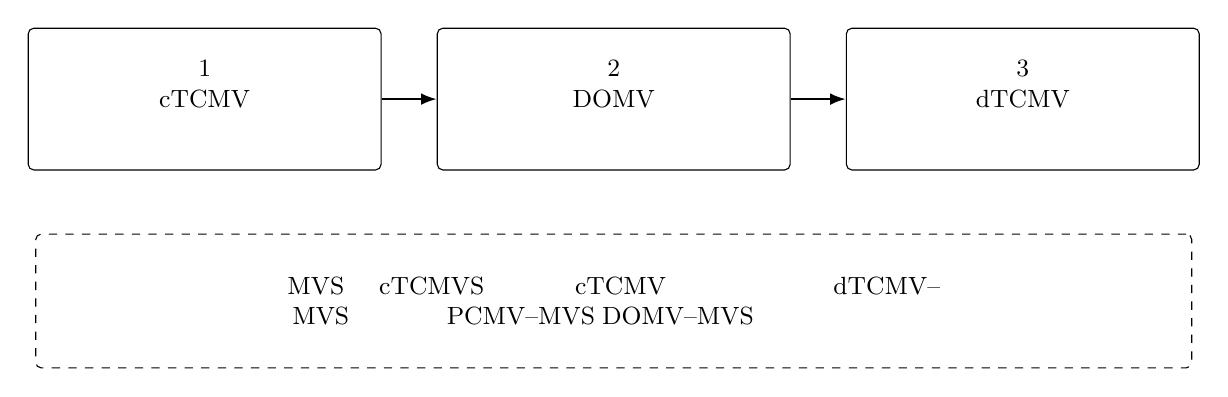
\begin{tikzpicture}[
  layer/.style={draw,rounded corners=2pt,align=center,text width=42mm,minimum height=18mm,inner sep=4pt,font=\small},
  research/.style={draw,dashed,rounded corners=2pt,align=center,text width=144mm,minimum height=17mm,inner sep=4pt,font=\small},
  arr/.style={-{Latex[length=2mm]},thick}
]
\node[layer] (l1) {第1層\\cTCMV\\標準デフォルト};
\node[layer,right=7mm of l1] (l2) {第2層\\DOMV\\定期的見直し};
\node[layer,right=7mm of l2] (l3) {第3層\\dTCMV\\総年金富に基づく個別化助言};
\node[research,below=8mm of l2] (mvs) {MVS研究拡張：cTCMVSは無制約解・クリップ近似でcTCMVと一致するが，厳密制約問題の一致は未証明である．dTCMV--MVSは係数感応度を本文で検証し，PCMV--MVS・DOMV--MVSは探索結果を公開する．現時点では運用層へ採用しない．};
\draw[arr] (l1) -- (l2);
\draw[arr] (l2) -- (l3);
\end{tikzpicture}
\caption{三層運用とMVSの位置づけ．MVSは運用層の追加または置換ではなく，説明可能な係数較正と数値安定性を確立するまで三層構造の外側で管理する研究拡張である．}
\label{fig:three-layer}
\end{figure}

\paragraph{実装上の原則．}
cTCMVは低コストなクリップ実装を許容しつつ射影差を定期監査する．DOMVは見直し時点ごとに厳密制約ソルバーまたは事前計算表を更新し，下方裾への影響を確認する．dTCMVは背景富・残高・残存期間に基づく選択制の個別化助言とし，上方参加と追加的下方リスクの適合性を管理する．MVSは説明可能な係数較正，非凹問題の独立再現および格子収束が確立するまで研究拡張にとどめる．

\section{限界と結論}
\label{sec:conclusion}

\subsection{限界と今後の課題}
本稿は一つの安全資産と一つのリスク資産，決定論的拠出，定数市場係数，取引費用なし，死亡・失業なしを仮定する．$H_t$は将来拠出と確定的給付の価値であり，実際の人的資本や確率的所得を完全に表すものではない．また，基準結果は月次離散モデルと採用格子の近似値であり，連続時間解への包括的収束は確認していない．MVSの正の係数に関する結果は非凹性と格子依存性を伴う探索的結果である．cTCMVSについては無制約解とクリップ近似の一致のみを確認済みの理論範囲とし，厳密制約問題での一致は未証明である．とくにPCMV--MVS・DOMV--MVSは運用提案ではなく公開資料として保存する．dTCMV--MVSの係数別グライドパスも，係数感応度を示す研究結果であって推奨較正ではない．PCMV・DOMVについては\ref{app:technical-proofs}で弱い存在性を整理する一方，cTCMV・dTCMVの状態依存両側制約下における大域的な均衡解の存在・一意性および正則性は未解決である．

付録Aでは四解概念の外部再現（dTCMVは公表終端分布の再構成）を示す．後退・前進整合性，質量保存および格子診断は公開リポジトリに収録するが，離散化の全組合せに対する包括的収束を示したものではない．優先すべき次段階は，(i)時間・状態・制御およびGauss--Hermite次数を同時に粗密化する包括的な格子安定性分析，(ii)DOMV・cTCMV・dTCMVに対する異なる離散化原理または独立ソルバーとの交差検証，(iii)MVS分枝の局所ターゲット・乗数・制御格子精緻化，(iv)確率的所得，死亡，複数資産，費用，デキュムレーションとの統合である．

\subsection{結論}
本稿は，DC固有の$0\leq\pi_t\leq X_t$制約下でPCMV，DOMV，cTCMV，dTCMVを統一的に扱い，無制約解，クリップ近似，厳密制約フィードバックを明確に分離した．理論上はいずれも局所射影構造を持つが，厳密制約フィードバックの射影は制約付き継続価値から得られ，別の無制約問題を事後的にクリップすることとは同じでない．

同一のGH誘導遷移核による後退・前進計算エンジンを用いることで，この差をグライドパス，終端分布，下方裾およびローリング条件付き分布まで一貫して伝播した．さらに，全分散の公式により，時点0の終端分散を各状態から先の平均条件付き分散と状態間の条件付き期待値分散へ分解した．この分解を基礎として，途中時点の現在残高からの条件付き平均，分位点，裾リスク，歪度および投資量をまとめるローリング条件付き成果指標を導入し，各戦略自身の経路と共通状態からの戦略差を可視化した．これにより，時点0の総分散でPCMVの設計効率を評価することと，評価日時点の状態からdTCMVなどの継続運用の便益・費用を評価することを両立できる．また，時点0の集団評価では混合される残存期間リスク，加入者間の状態格差，および将来方策の純粋な効果を区別できる．基準較正ではcTCMVのクリップ誤差は小さく，標準デフォルトの低コスト実装に適する．DOMVでは定期的再最適化の効果がクリップで再現されず，厳密制約ソルバーが必要となる．dTCMVは総年金富を参照して上方参加を加入者別に調整するが，下方リスクとの交換を伴うため，選択制の個別化助言としてガバナンスすべきである．

したがって，実務結論はPCMVを設計基準とし，cTCMV，DOMV，dTCMVを三つの運用層へ配置することである．MVSは第四層でも既存層の置換モデルでもない．cTCMVSの無制約解・クリップ近似における一致と厳密制約問題の未解決性，dTCMV--MVSの大きな係数感応度，およびPCMV--MVS・DOMV--MVSの数値的不安定性を踏まえ，現時点では三層構造の外側に置く研究拡張とする．本稿の価値は，複雑なモデルを一律に推奨することにあるのではない．そうではなく，どの場面で単純なクリップで十分であり，どの場面で厳密な数理計算が加入者成果とガバナンスに追加価値をもたらすのか，その区別を示した点にある．

\appendix
\renewcommand{\thesection}{付録\Alph{section}}
\section{再現可能性を支えるコード，数値データおよび検証資料}
\label{app:reproducibility}

\subsection{公開リポジトリと参照版}

本稿のPythonコード，主要なCSV・NPZデータ，図表生成スクリプトおよび実行手順は，次の公開リポジトリで公開している．
\begin{center}
\url{https://github.com/yoshi123027-del/dc-glidepath-ica2026}
\end{center}
本稿で使用したコードとデータの同一性を確保するため，参照版を次のコミットに固定する．これにより，リポジトリが将来更新された場合にも，本稿の数値結果に対応する実装を特定できる．
\begin{center}
\url{https://github.com/yoshi123027-del/dc-glidepath-ica2026/commit/d02af6cf693ec701396c2ef8879c4b1b52e25b70}
\end{center}
公開資料は，本稿の基準ケース，技術補論，PCMV・DOMVソルバー，cTCMV・dTCMVの拡張HJB計算，MVS拡張，ローリング条件付き評価，厳密制約フィードバックとクリップ近似の比較，表\ref{tab:dtcmv-u-decomposition}のU字型成因分解，および図表の再生成に必要なコードと数値データから構成される．公開資料には個人情報，非公開データおよび外部認証情報を含めていない．

本文の分析を補完する図は，次の補足図集に収録する．
\begin{center}
\url{https://github.com/yoshi123027-del/dc-glidepath-ica2026/tree/d02af6cf693ec701396c2ef8879c4b1b52e25b70/supplementary/figures}
\end{center}
補足図集には，終端富密度，上限制約の拘束確率と自由境界，射影差，ローリング条件付き評価，主要パラメータに対する感応度，およびMVS拡張の詳細を収録する．各図には，図が示す数値的事実，その数理的・実務的含意，ならびに解釈上の留意点を付記した．これらは本文の結論を代替するものではなく，結果の頑健性と数値的透明性を検討するための補完資料である．

\subsection{公開資料の構成}
公開リポジトリでは，ソルバー，較正，ローリング評価，感応度分析，図表生成および妥当性検証を機能別ディレクトリに整理している．完全再計算と保存済みCSV・NPZからの図表再生成の双方に対応し，各スクリプトの依存関係，実行順序および出力ファイルは，\path{README.md}，\path{scripts/README.md}および\path{CODEBOOK_JA.md}に記載する．本文では再現性の入口だけを示し，詳細なファイル一覧と実行コマンドはリポジトリを正本とする．

\subsection{四つのMV解概念に対する外部妥当性検証}
\label{app:four-model-validation}

本付録では，PCMV，DOMV，cTCMVおよびdTCMVのすべてについて，外部数値例の再現を行う．本稿固有の制約付き実装に対する後退・前進整合性，質量保存，格子安定性および自動回帰試験の詳細は公開リポジトリに収録する．\citet{vanStadenDangForsyth2021}の表5.1は，共通の市場設定と二つの目標平均の下で四解概念すべての終端富統計量を掲載している．したがって，外部再現をPCMVだけに限定せず，四解概念へ拡張する．ただし，公表情報の粒度は同一ではない．PCMV，DOMVおよびcTCMVは公表された閉形式から分布を独立に再計算できる一方，dTCMVは終端富が対数正規分布となることは示されているものの，数値的に解かれる時変係数の経路が表には掲載されていない．この相違を明示し，dTCMVについては公表された終端分布を再構成する外部検証と，本稿の制約付きソルバーに対する内部検証を組み合わせる．

\subsubsection{van Staden et al. (2021)表5.1の四解概念外部再現}

同論文の第5節に合わせて，初期富$w_0=100$，評価期間$T=10$年，$\mu=0.0816$，$\sigma=0.1863$，$r=0.00623$とし，拠出，取引費用およびレバレッジ制約を除いた．したがって，この検証は本稿の40年・拠出あり・$0\leq\pi\leq X$という基準ケースを再較正したものではなく，四解概念が共通に含む無制約特殊ケースの実装監査である．目標平均は同表と同じ125および250とした．

PCMVについては，同論文の式(3.6)および式(4.2)から反転対数正規分布を再計算した．DOMVおよびcTCMVについては，式(3.12)--(3.15)の正規終端分布と式(4.3)--(4.4)の目標平均に対応する分散回避係数から，平均，分散および裾統計量を閉形式で求めた．dTCMVについては，終端富が対数正規分布であるという式(3.16)を用いる．ただし，その時変係数を決める積分方程式の数値解は表5.1に掲載されていないため，公表平均$\bar w$と公表標準偏差$s_w$から
\begin{equation}
 s_L^2=\log\!\left(1+\frac{s_w^2}{\bar w^2}\right),
 \qquad
 \mu_L=\log \bar w-\frac12s_L^2
 \label{eq:dtcmv-external-lognormal-identification}
\end{equation}
により対数正規分布を同定し，中央値，歪度，超過尖度，VaR，LCVaR，下回り確率および条件付き平均を独立に再計算した．したがって，dTCMVの検証は公表された終端分布の再構成であり，未公表の時変係数経路そのものの独立再現ではない．この制御経路に関する検証は，公開リポジトリの後退・前進整合性および格子監査で補完する．

\begin{table}[H]
\centering
\caption{van Staden et al. (2021)表5.1の四解概念再現（各セルは公表値／再現値）}
\label{tab:vanstaden-all-mv-validation}
\scriptsize
\setlength{\tabcolsep}{3.3pt}
\begin{tabular}{@{}rlcccccc@{}}
\toprule
目標平均 & モデル & パラメータ & 平均 & 中央値 & 標準偏差 & $\VaR_{5\%}$ & $\mathrm{LCVaR}_{5\%}$ \\
\midrule
125 & PCMV  & $259/258.976$ & $125/125.000$ & $127/127.508$ & $9/9.130$ & $113/113.250$ & $97/97.412$ \\
    & DOMV  & $0.111/0.111411$ & $125/125.000$ & $125/125.000$ & $16/15.994$ & $99/98.692$ & $92/92.009$ \\
    & cTCMV & $0.044/0.044064$ & $125/125.000$ & $125/125.000$ & $15/14.517$ & $101/101.122$ & $95/95.056$ \\
    & dTCMV & $0.041/\text{--}$ & $125/125.000^{a}$ & $124/123.988$ & $16/16.000^{a}$ & $101/100.535$ & $96/95.424$ \\
\addlinespace
250 & PCMV  & $569/569.388$ & $250/250.000$ & $269/269.389$ & $71/70.577$ & $159/159.165$ & $37/36.726$ \\
    & DOMV  & $0.014/0.014412$ & $250/250.000$ & $250/250.000$ & $124/123.643$ & $47/46.626$ & $-5/-5.039$ \\
    & cTCMV & $0.006/0.005700$ & $250/250.000$ & $250/250.000$ & $112/112.223$ & $65/65.409$ & $19/18.515$ \\
    & dTCMV & $0.001/\text{--}$ & $250/250.000^{a}$ & $123/122.658$ & $444/444.000^{a}$ & $17/17.227$ & $11/11.342$ \\
\bottomrule
\end{tabular}
\begin{minipage}{0.98\textwidth}\vspace{2pt}\scriptsize
$^{a}$dTCMVの平均と標準偏差は，式\eqref{eq:dtcmv-external-lognormal-identification}により公表終端分布を同定するためのアンカーである．したがって，これら二つの一致は独立な再現結果ではない．
\end{minipage}
\end{table}

表5.1は原則として整数表示であるため，確率以外の公表値と再現値の差を1以下，確率の差を0.011以下とした．小数表示の分散回避パラメータについては$6\times10^{-4}$以下とした．モンテカルロ照合では，確率を原則$5\times10^{-4}$，平均・中央値・標準偏差を$\max(0.05,0.004|q|)$，最も標本誤差の大きい1--3\%下方裾を$\max(0.75,0.01|q|)$，その他の裾指標を$\max(0.35,0.006|q|)$とし，厚い右裾を持つdTCMVには標本変動を考慮した緩和幅を設定した（$q$は再現値）．表\ref{tab:vanstaden-all-mv-validation}の代表指標は，PCMV，DOMVおよびcTCMVについて公表された閉形式からの再計算と整合し，対応するモンテカルロ結果とも所定の許容差内で一致した．dTCMVについても，公表平均と標準偏差をアンカーとして再構成した対数正規終端分布から，中央値，分位点および裾指標を再現できた．ただし，これは公表終端分布の整合性確認であり，未公表の時変係数経路を独立に再現したものではない．全指標の照合値，許容差および内部監査結果は公開リポジトリの判定CSVに収録する．

\section{PCMV・DOMVの弱い存在性と検証定理の技術補論}
\label{app:technical-proofs}

本付録は，まずPCMVおよびDOMVについて，古典解を仮定しない弱い意味での存在性を整理する．その後，PCMVおよびDOMVについて第\ref{sec:theory}節で用いた検証論証を明示し，最後に四解概念に共通する自由境界と射影構造を整理する．弱い存在性は制御拡散，動的計画原理および粘性解の標準理論に基づく一方，PCMV・DOMVの局所フィードバック表示と検証定理は $C^{1,2}$ 級の候補関数と十分な可積分性を仮定する．したがって，本付録は本稿固有の自由境界について古典解の存在・一意性または滑らかさを主張するものではない．

\subsection{PCMVおよびDOMVの弱い存在性}
\label{app:pcmv-domv-existence}

以下では，$c:[0,T]\to[0,\infty)$ は有界連続，$D_T\geq0$ は定数とする．$x>0$ では $u_s=\pi_s/X_s$，$x=0$ では $u_s=0$ と置き，$[0,1]$ 値の進行可測過程 $u$ を正規化制御とする．このとき状態方程式は
\begin{equation}
 \dd X_s=\{c_s+(r+\beta u_s)X_s\}\dd s+\sigma u_sX_s\dd W_s,
 \qquad X_t=x\geq0
 \label{eq:normalized-controlled-state}
\end{equation}
となる．固定ターゲット $m$ に対する値関数を
\begin{equation}
 L^m(t,x)=\inf_{u}\E_{t,x}\!\left[(X_T^u+D_T-m)^2\right]
 \label{eq:app-weak-value}
\end{equation}
と定める．

\begin{proposition}[PCMVおよびDOMVの弱い存在性]
\label{prop:weak-existence-pcmv-domv}
上記の条件の下で，次が成り立つ．
\begin{enumerate}[label=(\roman*),leftmargin=2.2em]
 \item 任意の正規化制御 $u$ に対し，式\eqref{eq:normalized-controlled-state}は一意な非負強解を持つ．また，任意の $p\geq2$ とコンパクトな初期状態集合について，$\E[\sup_{t\leq s\leq T}|X_s^u|^p]$ は制御 $u$ に関して一様に有界である．
 \item $L^m$ は有限で，$(t,x,m)$ に関して連続かつ高々二次成長である．動的計画原理を満たし，HJB\eqref{eq:pcmv-hjb-x}の連続粘性解である．多項式成長を持つ連続粘性解のクラスで比較原理が成り立つなら，$L^m$ はそのクラスで一意である．さらに，コンパクト化した緩和制御のクラスには最適Markov制御が存在する．HJBの最小化点を与えるBorel可測な厳密制御選択が存在し，その閉ループSDEが適切に解ける場合には，最適厳密Markov制御を選べる．
 \item $\gamma>0$ に対して
 \begin{equation}
  \Psi_\gamma(t,x;m)
  =m-\frac{1}{2\gamma}-\frac{\gamma}{2}L^m(t,x)
  \label{eq:app-scalarized-envelope}
 \end{equation}
 と置くと，$m\mapsto\Psi_\gamma(t,x;m)$ は連続で，$|m|\to\infty$ のとき $-\infty$ へ収束する．したがって，スカラー化PCMVの外側最大化には少なくとも一つのターゲット $m_P^*(t,x)$ が存在する．
 \item 各 $(t,x)$ におけるDOMVの残存期間問題にも非空コンパクトな最適ターゲット集合
 \[
   \mathcal M_D^*(t,x)=\argmax_{m\in\mathbb R}\Psi_{\gamma_D}(t,x;m)
 \]
 が存在する．この対応からBorel可測な選択 $m_D^*(t,x)$ を取ることができ，各選択ターゲットに対する最適Markov制御の現在成分を接続することにより，弱い意味でのDOMVフィードバックを構成できる．
\end{enumerate}
本命題が主張しない点は，次の四つである：
\begin{enumerate}[label=(\alph*),leftmargin=2.2em,noitemsep,topsep=2pt]
 \item 任意に指定した目標平均$d$に対して，平均整合条件を満たす埋め込みターゲットが必ず存在すること，
 \item 値関数が$C^{1,2}$級であること，
 \item 自由境界が滑らかであること，
 \item 最適厳密フィードバックが一意かつ連続であること．
\end{enumerate}
\end{proposition}

\begin{proof}
正規化により制御集合は固定コンパクト区間 $[0,1]$ となる．式\eqref{eq:normalized-controlled-state}のドリフトと拡散係数は，$x$について制御一様にLipschitzかつ線形成長である．したがって，任意の進行可測制御に対して一意な強解が存在する．さらに，確率指数
\[
 Z_s=\exp\!\left(
  \int_t^s\!\left(r+\beta u_q-\frac12\sigma^2u_q^2\right)\dd q
  +\int_t^s\!\sigma u_q\dd W_q
 \right)
\]
を用いれば
\begin{equation}
 X_s=Z_s\left(x+\int_t^s Z_q^{-1}c_q\dd q\right)\geq0
 \label{eq:app-state-explicit}
\end{equation}
である．Burkholder--Davis--Gundy不等式とGronwall不等式を適用すれば，(i)の一様モーメント評価を得る．

終端損失は連続で二次成長を持ち，制御集合はコンパクトである．したがって，有限期間制御拡散の標準的な動的計画法により，値関数の有限性・連続性，動的計画原理および粘性解性が従う\citep{FlemingSoner2006}．厳密制御列を緩和制御へコンパクト化すれば最適緩和Markov制御が存在する．さらに，HJBハミルトニアンの最小化点についてBorel選択が可能で，選択後の閉ループ方程式が適切に解ける場合には，通常の検証・選択論法によって厳密Markov制御へ戻せる．これが(ii)である．

モーメント評価から，到達終端富 $W_T^u=X_T^u+D_T$ の一次モーメントは制御に関して一様に有界である．ある定数 $C_{t,x}<\infty$ に対し $\sup_u\E_{t,x}[W_T^u]\leq C_{t,x}$ であり，Jensenの不等式から
\[
 L^m(t,x)
 \geq \inf_u\{\E_{t,x}[W_T^u]-m\}^2
 \geq (|m|-C_{t,x})_+^2
\]
と評価できる．よって式\eqref{eq:app-scalarized-envelope}は $|m|\to\infty$ で $-\infty$ へ収束する．$L^m$ の連続性と合わせて最大値の存在が従い，(iii)を得る．同じ評価は各残存期間問題にも成り立つ．$\Psi_{\gamma_D}$ の共同連続性と局所一様な強制性から，最大化対応は非空コンパクト値かつ可測であり，可測最大値定理によりBorel選択 $m_D^*$ を取れる．各ターゲット問題の最適Markov制御の現在成分を接続すれば(iv)を得る．
\end{proof}

この命題は，PCMVおよびDOMVの存在性を，古典解と滑らかな自由境界の存在から切り離すためのものである．\citet{LiZhouLim2002}と\citet{LiXu2015}は制約付き平均--分散問題における粘性解・最適戦略の理論的背景を与え，\citet{GuanLiZhouZhou2022}は借入制約下の自由境界について古典解と正則性を示す類似結果を与える．ただし，後者はCRRA効用問題であり，本稿の二次損失HJBへ古典解の存在を直接移すものではない．

\subsection{PCMVおよびDOMVの古典解に基づく検証}
\label{app:pcmv-proof}

固定ターゲット $m$ と任意の許容制御 $\pi$ に対し，$X^\pi$ が有界領域を退出する時刻と二次変分を制御する時刻を用いて局所化し，その最小を $\tau_k$ とする．伊藤の公式より
\begin{equation}
 \E[v^m(\tau_k,X_{\tau_k}^\pi)]-v^m(t,x)
 =\E\int_t^{\tau_k}
 \left(v_s^m+\Lop^{\pi_s}v^m\right)(s,X_s^\pi)\dd s.
 \label{eq:app-pcmv-ito}
\end{equation}
HJB\eqref{eq:pcmv-hjb-x}から右辺の被積分関数は任意の $\pi$ に対して非負であり，最小化制御 $\pi^{m,*}$ に対してゼロである．多項式成長と一様可積分性により $k\to\infty$ とした後，終端条件を用いれば
\[
 v^m(t,x)\leq \E_{t,x}[(X_T^\pi+D_T-m)^2],
 \qquad
 v^m(t,x)=\E_{t,x}[(X_T^{\pi^{m,*}}+D_T-m)^2]
\]
を得る．ハミルトニアンの $\pi$ 依存部分は
\[
 q^m(\pi)=\beta v_x^m\pi+\frac12\sigma^2v_{xx}^m\pi^2
\]
であり，$v_{xx}^m>0$ の下で凸であるため，制約付き最小点は式\eqref{eq:pcmv-projection-x}である．平均制約付きPCMVは，本文で示した恒等式によりこの二次損失最小化へ帰着する．DOMVは，各 $(t,x)$ で同じ論証を残存期間問題へ適用し，その最初の制御を対角的に接続したものである．

\subsection*{自由境界と統一射影構造}

PCMV，cTCMV，dTCMVの各局所ハミルトニアンは，有効曲率の符号条件の下で一変数の凸または凹二次式になる．そのため，無制約の停留点が $0$ 以下，$[0,x]$ 内部，$x$ 以上のいずれに位置するかにより，下限制約領域，内点領域，上限制約領域へ分かれる．停留点は制約付き値関数または均衡モーメントの微分から計算されるため，切替集合は未知関数に依存する自由境界である．この共通構造は射影形式を統一するが，無制約解のクリップ近似と厳密制約フィードバックを同一にするものではない．


\section*{謝辞および開示}
生成AIツールを，TeX編集，Markov--Gauss--Hermiteエンジンのコード実装，論文構成案および推敲，周辺調査，論理破綻の検証に使用した．理論，数値結果，および最終内容に対する責任は著者が負う．

\begingroup
\footnotesize
\setlength{\bibsep}{1pt}
\begin{thebibliography}{99}
\footnotesize
\bibitem[Abramowitz and Stegun(1972)]{AbramowitzStegun1972}
Abramowitz, M., and Stegun, I. A. (1972).
\emph{Handbook of Mathematical Functions with Formulas, Graphs, and Mathematical Tables}.
Dover.

\bibitem[Australian Prudential Regulation Authority(2023)]{APRASPS530}
Australian Prudential Regulation Authority (2023).
\emph{Prudential Standard SPS 530: Investment Governance}.
\href{https://www.apra.gov.au/standards/sps-530}{Official standard}.

\bibitem[Australian Prudential Regulation Authority(2025)]{APRASPS515}
Australian Prudential Regulation Authority (2025).
\emph{Prudential Standard SPS 515: Strategic Planning and Member Outcomes}.
\href{https://www.apra.gov.au/standards/sps-515}{Official standard}.

\bibitem[Basak and Chabakauri(2010)]{BasakChabakauri2010}
Basak, S., and Chabakauri, G. (2010).
Dynamic mean--variance asset allocation.
\emph{Review of Financial Studies}, 23(8), 2970--3016.

\bibitem[Basu et al.(2011)]{BasuByrneDrew2011}
Basu, A. K., Byrne, A., and Drew, M. E. (2011).
Dynamic lifecycle strategies for target date retirement funds.
\emph{Journal of Portfolio Management}, 37(2), 83--96.

\bibitem[Bensoussan et al.(2014)]{BensoussanWongYamYung2014}
Bensoussan, A., Wong, K. C., Yam, S. C. P., and Yung, S. P. (2014).
Time-consistent portfolio selection under short-selling prohibition: From discrete to continuous setting.
\emph{SIAM Journal on Financial Mathematics}, 5(1), 153--190.

\bibitem[Bjork and Murgoci(2014)]{BjorkMurgoci2014}
Bjork, T., and Murgoci, A. (2014).
A theory of Markovian time-inconsistent stochastic control in discrete time.
\emph{Finance and Stochastics}, 18, 545--592.

\bibitem[Bjork et al.(2014)]{BjorkMurgociZhou2014}
Bjork, T., Murgoci, A., and Zhou, X. Y. (2014).
Mean--variance portfolio optimization with state-dependent risk aversion.
\emph{Mathematical Finance}, 24(1), 1--24.

\bibitem[Bjork et al.(2017)]{BjorkKhapkoMurgoci2017}
Bjork, T., Khapko, M., and Murgoci, A. (2017).
On time-inconsistent stochastic control in continuous time.
\emph{Finance and Stochastics}, 21, 331--360.

\bibitem[Bodie et al.(1992)]{BodieMertonSamuelson1992}
Bodie, Z., Merton, R. C., and Samuelson, W. F. (1992).
Labor supply flexibility and portfolio choice in a life-cycle model.
\emph{Journal of Economic Dynamics and Control}, 16(3--4), 427--449.

\bibitem[Cairns et al.(2006)]{CairnsBlakeDowd2006}
Cairns, A. J. G., Blake, D., and Dowd, K. (2006).
Stochastic lifestyling: Optimal dynamic asset allocation for defined contribution pension plans.
\emph{Journal of Economic Dynamics and Control}, 30(5), 843--877.

\bibitem[Cocco et al.(2005)]{CoccoGomesMaenhout2005}
Cocco, J. F., Gomes, F. J., and Maenhout, P. J. (2005).
Consumption and portfolio choice over the life cycle.
\emph{Review of Financial Studies}, 18(2), 491--533.

\bibitem[Di Giacinto et al.(2014)]{DiGiacintoFedericoGozziVigna2014}
Di Giacinto, M., Federico, S., Gozzi, F., and Vigna, E. (2014).
Income drawdown option with minimum guarantee.
\emph{European Journal of Operational Research}, 234(3), 610--624.
doi:10.1016/j.ejor.2013.10.026.

\bibitem[Estrada(2019)]{Estrada2019}
Estrada, J. (2019).
The glidepath illusion: An international perspective.
\emph{Journal of Portfolio Management}, 45(6), 52--64.

\bibitem[Falcone and Ferretti(2014)]{FalconeFerretti2014}
Falcone, M., and Ferretti, R. (2014).
\emph{Semi-Lagrangian Approximation Schemes for Linear and Hamilton--Jacobi Equations}.
SIAM.

\bibitem[Ferreira Morici and Vigna(2025)]{FerreiraMoriciVigna2025}
Ferreira Morici, H., and Vigna, E. (2025).
Optimal additional voluntary contribution in DC pension schemes to manage inadequacy risk.
\emph{Decisions in Economics and Finance}, 48(2), 1031--1063.
doi:10.1007/s10203-024-00451-3.

\bibitem[Fleming and Soner(2006)]{FlemingSoner2006}
Fleming, W. H., and Soner, H. M. (2006).
\emph{Controlled Markov Processes and Viscosity Solutions}, 2nd ed.
Springer.

\bibitem[Forsyth and Vetzal(2019)]{ForsythVetzal2019}
Forsyth, P. A., and Vetzal, K. R. (2019).
Optimal asset allocation for retirement saving: Deterministic vs. time consistent adaptive strategies.
\emph{Applied Mathematical Finance}, 26(1), 1--37.

\bibitem[Guan et al.(2022)]{GuanLiZhouZhou2022}
Guan, C., Li, X., Zhou, R., and Zhou, W. (2022).
Free boundary problem for an optimal investment problem with a borrowing constraint.
\emph{Journal of Industrial and Management Optimization}, 18(3), 1915--1934.

\bibitem[Haberman and Vigna(2002)]{HabermanVigna2002}
Haberman, S., and Vigna, E. (2002).
Optimal investment strategies and risk measures in defined contribution pension schemes.
\emph{Insurance: Mathematics and Economics}, 31(1), 35--69.
doi:10.1016/S0167-6687(02)00128-2.

\bibitem[H{\o}jgaard and Vigna(2007)]{HojgaardVigna2007}
H{\o}jgaard, B., and Vigna, E. (2007).
Mean--variance portfolio selection and efficient frontier for defined contribution pension schemes.
\emph{Research Report Series}, R-2007-13, Department of Mathematical Sciences, Aalborg University.

\bibitem[ICA2026 Scientific Committee(2026)]{ICA2026Guidance}
ICA2026 Scientific Committee (2026).
\emph{Guidance for Preparing a Paper}.
33rd International Congress of Actuaries, Tokyo.

\bibitem[Institute of Actuaries of Japan(2026)]{ICA2026PeerReview}
Institute of Actuaries of Japan (2026).
\emph{Guidelines for Peer Review}.
33rd International Congress of Actuaries, Tokyo.

\bibitem[International Actuarial Association(2013)]{IAA2013Role}
International Actuarial Association (2013).
\emph{The Role of the Actuary}.
Ottawa: International Actuarial Association.

\bibitem[International Actuarial Association(2016)]{IAA2016Profession}
International Actuarial Association (2016).
\emph{Defining the Actuarial Profession}.
Ottawa: International Actuarial Association.

\bibitem[International Actuarial Association(2021)]{IAA2021DCRoadmap}
International Actuarial Association (2021).
\emph{Comments on the Consultation on the OECD Roadmap for the Good Design of Defined Contribution Retirement Savings Plans}.
Ottawa: International Actuarial Association.

\bibitem[Judd(1998)]{Judd1998}
Judd, K. L. (1998).
\emph{Numerical Methods in Economics}.
MIT Press.

\bibitem[Kushner and Dupuis(2001)]{KushnerDupuis2001}
Kushner, H. J., and Dupuis, P. G. (2001).
\emph{Numerical Methods for Stochastic Control Problems in Continuous Time}, 2nd ed.
Springer.

\bibitem[Li and Ng(2000)]{LiNg2000}
Li, D., and Ng, W.-L. (2000).
Optimal dynamic portfolio selection: Multiperiod mean--variance formulation.
\emph{Mathematical Finance}, 10(3), 387--406.

\bibitem[Li and Xu(2015)]{LiXu2015}
Li, X., and Xu, Z. Q. (2015).
Continuous-time mean--variance portfolio selection with constraints on wealth and portfolio.
\emph{arXiv preprint arXiv:1507.06850}.

\bibitem[Li et al.(2002)]{LiZhouLim2002}
Li, X., Zhou, X. Y., and Lim, A. E. B. (2002).
Dynamic mean--variance portfolio selection with no-shorting constraints.
\emph{SIAM Journal on Control and Optimization}, 40(5), 1540--1555.

\bibitem[Markowitz(1952)]{Markowitz1952}
Markowitz, H. (1952).
Portfolio selection.
\emph{Journal of Finance}, 7(1), 77--91.

\bibitem[Menoncin and Vigna(2017)]{MenoncinVigna2017}
Menoncin, F., and Vigna, E. (2017).
Mean--variance target-based optimisation for defined contribution pension schemes in a stochastic framework.
\emph{Insurance: Mathematics and Economics}, 76, 172--184.
doi:10.1016/j.insmatheco.2017.08.002.

\bibitem[Menoncin and Vigna(2020)]{MenoncinVigna2020}
Menoncin, F., and Vigna, E. (2020).
Mean--variance dynamic optimality for DC pension schemes.
\emph{European Actuarial Journal}, 10, 125--148.
doi:10.1007/s13385-020-00226-1.

\bibitem[Merton(1969)]{Merton1969}
Merton, R. C. (1969).
Lifetime portfolio selection under uncertainty: The continuous-time case.
\emph{Review of Economics and Statistics}, 51(3), 247--257.

\bibitem[Ministry of Health, Labour and Welfare(2026a)]{MHLWDCAct}
Ministry of Health, Labour and Welfare (2026a).
\emph{Defined Contribution Pension Act}, Articles 23--24-2 (current consolidated text, accessed July 2026).
\href{https://www.mhlw.go.jp/web/t_doc?dataId=85aa2545&dataType=0&pageNo=1}{Official consolidated text}.

\bibitem[Mu et al.(2019)]{MuTianYang2019}
Mu, C., Tian, W., and Yang, J. (2019).
Portfolio choice with skewness preference and wealth-dependent risk aversion.
\emph{Quantitative Finance}, 19(11), 1905--1919.
doi:10.1080/14697688.2019.1592214.

\bibitem[OECD(2025)]{OECD2025PensionMarkets}
OECD (2025).
\emph{Pension Markets in Focus 2025}.
Paris: OECD Publishing.
doi:10.1787/b095d0a0-en.

\bibitem[Pedersen and Peskir(2017)]{PedersenPeskir2017}
Pedersen, J. L., and Peskir, G. (2017).
Optimal mean--variance portfolio selection.
\emph{Mathematics and Financial Economics}, 11, 137--160.

\bibitem[The Pensions Regulator(2024)]{TPRDCInvestment2024}
The Pensions Regulator (2024).
\emph{Investment Governance in DC Schemes}.
\href{https://www.thepensionsregulator.gov.uk/document-library/scheme-management-detailed-guidance/funding-and-investment-detailed-guidance/investment-guide-for-dc-pension-schemes}{Official guidance}.

\bibitem[Thinking Ahead Institute(2026)]{TAI2026GPAS}
Thinking Ahead Institute (2026).
\emph{Global Pension Assets Study 2026}.
London: Thinking Ahead Institute and WTW.

\bibitem[U.S. Department of Labor(2007)]{USDOLQDIA}
U.S. Department of Labor (2007).
\emph{Default Investment Alternatives under Participant-Directed Individual Account Plans: Final QDIA Rule and Guidance}.
Employee Benefits Security Administration.
\href{https://www.dol.gov/agencies/ebsa/laws-and-regulations/laws/pension-protection-act}{Official final-rule and guidance page}.

\bibitem[van Staden et al.(2021)]{vanStadenDangForsyth2021}
van Staden, P. M., Dang, D.-M., and Forsyth, P. A. (2021).
On the distribution of terminal wealth under dynamic mean--variance optimal investment strategies.
\emph{SIAM Journal on Financial Mathematics}, 12(2), 566--603.
doi:10.1137/20M1338241.

\bibitem[Viceira(2001)]{Viceira2001}
Viceira, L. M. (2001).
Optimal portfolio choice for long-horizon investors with nontradable labor income.
\emph{Journal of Finance}, 56(2), 433--470.

\bibitem[Vigna and Haberman(2001)]{VignaHaberman2001}
Vigna, E., and Haberman, S. (2001).
Optimal investment strategy for defined contribution pension schemes.
\emph{Insurance: Mathematics and Economics}, 28(2), 233--262.
doi:10.1016/S0167-6687(00)00077-9.

\bibitem[Vigna(2014)]{Vigna2014}
Vigna, E. (2014).
On efficiency of mean--variance based portfolio selection in DC pension schemes.
\emph{Quantitative Finance}, 14(2), 237--258.
doi:10.1080/14697688.2012.708778.

\bibitem[Vigna(2020)]{Vigna2020}
Vigna, E. (2020).
On time consistency for mean--variance portfolio selection.
\emph{International Journal of Theoretical and Applied Finance}, 23(6), 2050042.
doi:10.1142/S0219024920500429.

\bibitem[Wang and Forsyth(2012a)]{WangForsyth2012}
Wang, J., and Forsyth, P. A. (2012a).
Numerical solution of the Hamilton--Jacobi--Bellman formulation for continuous time mean variance asset allocation.
\emph{Journal of Economic Dynamics and Control}, 36(2), 207--230.

\bibitem[Wang and Forsyth(2012b)]{WangForsyth2012Comparison}
Wang, J., and Forsyth, P. A. (2012b).
Comparison of mean variance like strategies for optimal asset allocation problems.
\emph{International Journal of Theoretical and Applied Finance}, 15(2), 1250014.

\bibitem[Zhou and Li(2000)]{ZhouLi2000}
Zhou, X. Y., and Li, D. (2000).
Continuous-time mean--variance portfolio selection: A stochastic LQ framework.
\emph{Applied Mathematics and Optimization}, 42, 19--33.
\end{thebibliography}
\endgroup

\end{document}
